\documentclass[12pt,a4paper]{report}
\usepackage[utf8]{inputenc}
\usepackage[T1]{fontenc}
\usepackage{lmodern}
\usepackage[
    colorlinks=true,     % no boxes, just coloured text
    linkcolor=blue,      % colour for internal links (TOC, equations, etc.)
    citecolor=teal,      % colour for citations
    urlcolor=magenta     % colour for URLs
]{hyperref}
\usepackage{microtype}
\usepackage[margin=1in]{geometry}
\usepackage{amsmath,amssymb,amsthm}
\usepackage{graphicx}
\usepackage{booktabs}
\usepackage{caption}
\usepackage{subcaption}
\usepackage{listings}
\usepackage{xcolor}
\usepackage{algorithm}
\usepackage{algpseudocode}
\usepackage{csvsimple}
\usepackage{pgfplots}
\pgfplotsset{compat=1.18}
\usepackage[capitalise]{cleveref}
\usepackage{tikz}
\usepackage{eso-pic}
\usepackage{background}
\usepackage{xcolor}  % for custom colours
\usepackage{algpseudocode}
\usepackage{upquote}
\usepackage{tcolorbox}
\usepackage{float}
\usepackage[numbers]{natbib}


\lstset{
  language=Python,                      % language for syntax highlighting
  basicstyle=\ttfamily\small,           % font style: typewriter, small size
  numbers=left,                         % line numbers on the left
  numberstyle=\tiny,                    % font size for line numbers
  stepnumber=1,                         % line number step
  numbersep=5pt,                        % distance between line numbers and code
  frame=single,                         % draw a frame around code
  rulecolor=\color{black},              % frame color
  breaklines=true,                      % allow line breaking
  breakatwhitespace=true,               % only break at whitespace if possible
  showstringspaces=false,               % don't mark spaces in strings
  tabsize=4,                            % set tab width to 4 spaces
  captionpos=b,                         % position of caption (b = bottom, t = top)
  columns=fullflexible,                 % better spacing for monospace text
  keepspaces=true,                      % keep spaces in code for indentation
  upquote=true,                         % use straight quotes instead of curly
  keywordstyle=\color{blue},            % style for keywords
  commentstyle=\color{gray},            % style for comments
  stringstyle=\color{red},              % style for strings
% identifierstyle=\color{teal},         % variables/functions
  emph={coinChangeGreedy, coinChangeDP, sort},               
  emphstyle=\color{orange}\bfseries,    % highlight specific names
  showtabs=false,                       % don't show special markers for tabs
  showspaces=false                      % don't show special markers for spaces
}

\newtheorem{definition}{Definition}
\newtheorem{theorem}{Theorem}

\newcommand\CoverBackground{%
    \put(0,0){%
        \parbox[b][\paperheight]{\paperwidth}{%
            \vfill
            \centering
            
\includegraphics[width=\paperwidth,height=\paperheight]{cover.jpg}%
            \vfill
        }%
    }%
}
\backgroundsetup{
  scale=1,
  angle=0,
  opacity=0.5,
  contents={
\includegraphics[width=\paperwidth,height=\paperheight]{main_bg.jpg}}
}      
\begin{document}

\begin{titlepage}
    \AddToShipoutPicture*{\CoverBackground}
    \centering
    \vspace*{6cm}
    
    {\Huge\bfseries DAA- Coin Change Problem \par}
    \vspace{1.5cm}
    
    {\Large Nanchaku \par}
    \vspace{0.5cm}
    
    {\large Indian Statistical Institute Bangalore \par}
    \vspace{2cm}
    
    {\Large Submitted to Dr. Jaya Sreevalsan Nair \par}
    \vspace{6cm}

    {\large \href{https://github.com/ItzKanashii/Coin-Change}{Our project's Github Repository Link} \par}
    \vspace{1cm}

    {\large \href{https://github.com/ItzKanashii/Coin-Change/blob/main/README.md}{README} \par}
    \vfill
\end{titlepage}
\ClearShipoutPicture
\begin{flushright}
\textit{"Program testing can be used to show the presence of bugs but never to show their absence." \newline Edsger Dijkstra}
\end{flushright}

\chapter*{Acknowledgment \centering}

We express our sincere gratitude to Dr. Jaya Sreevalsan Nair, our course instructor, for their guidance and support throughout this project. Their insights on algorithm design and analysis greatly aided in structuring the experiments and interpreting the results. We also thank our peers for their valuable discussions and feedback, which helped refine our implementations and presentation.

\chapter*{Declaration of Originality \centering}
We hereby declare that this project is our own work and that we have not received any unauthorized external help. All sources and references used are acknowledged.\newline
\vfill
Team Nanchaku \newline
\begin{itemize}
    \item \href{https://github.com/ItzKanashii/Coin-Change}{Pushpender Chauhan}\hfill \textit{Bmat2334}
    \item \href{https://github.com/ItzKanashii/Coin-Change}{Vishal Vikram Parth}\hfill \textit{Bmat2347}
\end{itemize}
\tableofcontents
\setcounter{chapter}{-1}
\chapter{Introduction \centering}
The coin change problem is a fundamental question in algorithm design: given a set of coin denominations and a target amount, determine the minimum number of coins needed to make that amount. This problem has both theoretical interest in computer science and practical importance in financial systems, where efficiency in currency transactions is essential.

One common approach to the problem is the greedy algorithm, which repeatedly selects the largest coin denomination not exceeding the remaining amount. For certain coin systems, known as canonical systems, this method always produces an optimal solution. Many real-world currencies are designed to be canonical, making greedy algorithm efficient and effective in practice. However, for non-canonical systems, our algorithm may fail to minimize the number of coins, motivating the need for more general methods.

An alternative is the dynamic programming algorithm, which systematically explores all possibilities to guarantee the minimum number of coins regardless of the coin system. Although less efficient than greedy in terms of time complexity, dynamic programming ensures correctness even when denominations are non-canonical.

This project develops and analyzes both approaches. For the greedy algorithm, we provide pseudocode, a formal proof of correctness for canonical systems, and a Python implementation applied to real-world coin denominations. We then implement the dynamic programming approach, presenting its pseudocode, Python code, and experimental evaluation on both canonical and non-canonical coin systems. Finally, we compare the two algorithms using empirical results and graphical visualizations to highlight the trade-off between efficiency and optimality.


\chapter{Greedy Algorithm for Coin Change\centering}
\section{Problem Description in the Greedy Setting}
\label{sec:greedy-algo}

The \textbf{coin change problem} can be stated formally as follows:

\begin{itemize}
    \item \textbf{Input:} A set of coin denominations
    \[
    \mathcal{D} = \{d_1, d_2, \dots, d_k\}, \quad d_1 < d_2 < \cdots < d_k,
    \]
    where each $d_i \in \mathbb{N}$ and typically $d_1 = 1$ to ensure that every amount can be represented, and a target value $N \in \mathbb{N}$.
    \item \textbf{Objective:} Find the minimum number of coins from $\mathcal{D}$ whose sum equals $N$.
\end{itemize}

\subsection{Greedy Algorithm}

The \textbf{greedy algorithm} addresses this problem by always selecting the largest denomination that does not exceed the remaining amount. Formally, the algorithm works as follows: starting with amount $N$, choose the maximum $d_j \in \mathcal{D}$ such that $d_j \leq N$, subtract $d_j$ from $N$, and repeat until the remaining amount is zero.

\subsection{Canonical and Non-Canonical Coin Systems}

The effectiveness of the greedy algorithm depends on the structure of the coin set $\mathcal{D}$.\cite{cai2008}

\begin{definition}[Canonical Coin System]
A coin system $\mathcal{D}$ is called \textbf{canonical} if, for every target amount $N \in \mathbb{N}$, the greedy algorithm produces an \textbf{optimal solution}, i.e., a solution using the minimum possible number of coins.
\end{definition}

\begin{definition}[Non-Canonical Coin System]
A coin system $\mathcal{D}$ is called \textbf{non-canonical} if there exists at least one target amount $N \in \mathbb{N}$ for which the greedy algorithm does not yield the minimum number of coins.
\end{definition}

\subsection{Representation and Greedy Representation}

\begin{definition}[Representation]
A \textbf{representation} of a target amount $N$ is a vector $x = (x_1, \dots, x_k)$ with $x_i \in \mathbb{Z}_{\ge 0}$ such that
\[
\sum_{i=1}^{k} x_i d_i = N.
\]
The \textbf{size} of a representation is $|x| = \sum_{i=1}^{k} x_i$.
\end{definition}

\begin{definition}[Greedy Representation]
The \textbf{greedy representation} $g(N)$ of $N$ is obtained by repeatedly choosing the largest coin $d_j \le$ remaining amount until the remaining amount becomes zero.
\end{definition}

\subsection{Finite Test for Canonicity}

\begin{theorem}[Finite Test for Canonicity]
Let $\mathcal{D} = \{d_1, \dots, d_k\}$ with $d_1 = 1$ and $d_1 < \dots < d_k$. 
Then $\mathcal{D}$ is canonical if and only if the greedy representation is optimal for every amount
\[
1 \le N \le d_k + d_{k-1} - 1.
\]
\end{theorem}

\begin{proof}
Assume that $\mathcal{D}$ is not canonical. Let $M$ be the \textit{smallest} amount for which the greedy representation $g(M)$ is not optimal. Let $o = (o_1, \dots, o_k)$ be an optimal representation of $M$, i.e.,
\[
|o| < |g(M)|.
\]

Let 
\[
r = \max\{ i : g_i(M) \neq o_i \}.
\]
By definition, $g_r(M) > o_r$ and $g_i(M) = o_i$ for all $i > r$. Define
\[
\Delta := \sum_{i=1}^{r} (g_i(M) - o_i)d_i.
\]
This is the excess value of greedy coins up to index $r$ and satisfies
\[
\Delta = \sum_{i=r+1}^{k} (o_i - g_i(M)) d_i \ge d_{r+1},
\]
because the right-hand side is a positive combination of coins with indices greater than $r$.

On the other hand, by definition of greedy, for $i \le r$ we have
\[
g_i(M) \le \left\lfloor \frac{d_{i+1}-1}{d_i} \right\rfloor.
\]
From this, it follows that
\[
\Delta = \sum_{i=1}^{r} (g_i(M) - o_i)d_i \le \sum_{i=1}^{r} g_i(M)d_i \le d_{r+1}-1.
\]

The inequalities
\[
\Delta \ge d_{r+1} \quad \text{and} \quad \Delta \le d_{r+1}-1
\]
are contradictory unless $r = k-1$. Then we have
\[
M < d_k + d_{k-1}.
\]

Therefore, if greedy fails for some amount, it must fail for some amount $N < d_k + d_{k-1}$. Conversely, if greedy succeeds for all amounts $1 \le N < d_k + d_{k-1}$, it succeeds for all $N$, proving the theorem.
\end{proof}

This theorem provides a finite algorithmic test for canonicity: check all amounts up to $d_k + d_{k-1} - 1$. If greedy succeeds for all of them, the system is canonical; otherwise, it is non-canonical.


\subsection*{Examples}

\begin{itemize}
    \item \textbf{Canonical system:} The United States coin denominations 
    \[
    \{1, 5, 10, 25\}
    \]
    form a canonical system. For any amount $N$, the greedy method gives the optimal solution. For example, for $N = 30$, greedy method selects $25 + 5$, which is indeed minimal.

    \item \textbf{Non-canonical system:} Consider 
    \[ \mathcal{D} = \{1, 3, 4\}.\] 
    For $N = 6$, the greedy algorithm selects $4 + 1 + 1$ (3 coins), but the optimal solution is $3 + 3$ (2 coins). Thus, this system is non-canonical.
\end{itemize}

This problem description sets up the framework for presenting the greedy algorithm formally, proving its correctness in canonical systems, and demonstrating counterexamples in non-canonical systems.


\section{Pseudocode for Coin Change using Greedy Approach}

\begin{algorithm}
\caption{Greedy Algorithm for Coin Change}
\begin{algorithmic}[1]
\Procedure{CoinChangeGreedy}{$coins, target$}
    \State \Comment{$coins$ is assumed to be sorted in descending order}
    \State $count \gets 0$ \Comment{Initialize the coin counter}
    
    \For{$coin \in coins$}
        \While{$target \ge coin$}
            \State $target \gets target - coin$ \Comment{Subtract coin value from remaining target}
            \State $count \gets count + 1$ \Comment{Increment the coin count}
        \EndWhile
    \EndFor
    
    \If{$target = 0$}
        \State \Return $count$ \Comment{Successfully formed target with selected coins}
    \Else
        \State \Return $-1$ \Comment{Target cannot be formed with given coins}
    \EndIf
\EndProcedure
\end{algorithmic}
\end{algorithm}

\section{Proof of Correctness of the Greedy Coin Change Algorithm}

\paragraph{Algorithm.}
The procedure \textsc{CoinChangeGreedy} takes input as a set of coin denominations 
\[
coins = \{c_1, c_2, \dots, c_k\}, \quad c_1 > c_2 > \dots > c_k > 0,
\]
and a target amount $T \geq 0$. It repeatedly subtracts the largest possible coin until the target is reached or no further subtraction is possible. The output is the number of coins used, or $-1$ if no representation exists.

\subsection*{Termination}
At each subtraction step, the algorithm decreases the value of \texttt{target} by at least $1$ (since $c_k \geq 1$). Hence, the \texttt{while} loop cannot be executed indefinitely.  
Therefore, the algorithm always terminates.

\subsection*{Partial Correctness}
We prove by induction on the structure of the loops that if the algorithm returns a non-negative integer $count$, then the chosen set of coins indeed sums up to $T$.

\begin{itemize}
    \item \textbf{Initialization:} Before the first iteration, \texttt{target} $=T$ and \texttt{count} $=0$. The invariant ``$\texttt{target} + \texttt{sum of chosen coins} = T$'' holds.
    \item \textbf{Maintenance:} Suppose the invariant holds before subtracting $coin$. Then after one subtraction, the new target is
    \[
    \texttt{target}_{new} = \texttt{target}_{old} - coin,
    \]
    and the sum of chosen coins increases by $coin$. Thus,
    \[
    \texttt{target}_{new} + \texttt{sum of chosen coins}_{new} = T.
    \]
    Thus, the invariant is preserved.
    \item \textbf{Termination:} When the loops finish, if \texttt{target}$=0$, then
    \[
    0 + \texttt{sum of chosen coins} = T,
    \]
    i.e. the coins selected sum exactly to $T$. The algorithm then returns the number of coins used.
\end{itemize}

Hence, whenever the algorithm returns a nonnegative integer, it is a valid representation of $T$.

\subsection{Optimality in Canonical Coin Systems}
The greedy algorithm does not always yield an optimal solution for arbitrary coin systems.  
However, in \emph{canonical coin systems} (for example, the U.S. coin system $\{25,10,5,1\}$), the greedy strategy is known to be optimal. \\

\textbf{Theorem:}
Let $coins=\{c_1>c_2>\cdots>c_k=1\}$ be a canonical coin system. For every integer target $T\ge0$, the greedy algorithm produces a representation of $T$ with the minimum possible number of coins.

\begin{proof}
Let $G$ be the multiset of coins produced by the greedy algorithm for the target $T$. Let $g_i$ denote the number of coins of denomination $c_i$ in $G$. Let $O$ be an optimal multiset of coins for $T$ with minimal total number of coins and let $o_i$ denote the number of coins of denomination $c_i$ in $O$.

If $g_i=o_i$ for all $i$ then $G$ is optimal and we are done. Suppose not. Let
\[
r=\max\{\,i: g_i\ne o_i\,\}
\]
be the largest index where $G$ and $O$ differ. By definition of greedy, at denomination $c_r$ the greedy algorithm took as many $c_r$ coins as possible given the remaining amount; therefore $g_r>o_r$ (if $g_r<o_r$ then $O$ would have more of the larger coin than greedy, contradicting greedy's maximal choice at earlier steps). Hence $g_r\ge o_r+1$.

Consider the contribution of denominations strictly smaller than $c_r$ in $O$. Since the total values of $G$ and $O$ are equal,
\[
\sum_{i<r} (o_i-g_i)c_i = (g_r-o_r)c_r + \sum_{i>r} (g_i-o_i)c_i.
\]
The rightmost sum is nonnegative because for indices larger than $r$ we have $g_i=o_i$ by the maximality of $r$. Thus, the left side is at least $(g_r-o_r)c_r\ge c_r$.
Hence, the coins of denominations $<c_r$ appearing in $O$ have a total value of at least $c_r$.

Replace in $O$ a minimal sub-multiset of coins of denomination $<c_r$ whose total value is at least $c_r$ by a single coin of value $c_r$. Because each replaced coin has value $<c_r$, the number of replaced coins is at least $1$. Therefore, this replacement does not increase the total number of coins in $O$ and strictly increases the count $o_r$ by at least $1$. Repeat this replacement until $o_r$ becomes $g_r$. Each replacement preserves feasibility and does not increase the coin count. After finitely many such replacements, we obtain another optimal solution in which $o_r=g_r$ while the total number of coins have not increased.

Apply the same procedure for the next largest index where the modified $O$ and $G$ differ. Iterating this exchange process from the largest differing index downwards transforms $O$ into $G$ without increasing the number of coins. Since $O$ was assumed to be optimal, $G$ cannot have more coins than $O$. Hence $G$ is also optimal.
\end{proof}

\subsection{Conclusion}
\begin{itemize}
    \item The algorithm always terminates.
    \item If it returns a nonnegative integer, the selected coins sum to the target.
    \item In canonical coin systems, the returned solution is optimal.
    \item If it returns $-1$, no such representation exists with the given coin set.
\end{itemize}
Therefore, the algorithm is correct under the canonical coin system assumption.

\section{Time and Space Complexity of the Greedy Coin-Change Algorithm}

Let \(k = |coins|\), \(T\) be the target amount, \(c_{\min} = \min(coins) > 0\), and let \(m\) denote the number of coins the algorithm actually selects. Since every selected coin reduces the remaining target by at least \(c_{\min}\), we have \(m \le \lfloor T / c_{\min} \rfloor\). Scanning through all denominations costs \(\Theta(k)\). 
Each subtraction and counter-increment costs \(O(1)\), so the total cost of the greedy selection loop is \(\Theta(m)\). Therefore, the overall time complexity is \(\Theta(k + m)\).

\subsection{Best Case}
The best case occurs when the target \(T = 0\) or when \(T\) equals one of the coin denominations and the algorithm immediately selects it. In this case:

\begin{itemize}
    \item The algorithm scans through the coin list exactly once (\(\Theta(k)\)).
    \item The while-loop executes at most once or not at all (\(\Theta(1)\)).
\end{itemize}

Hence, the total best-case time complexity is
\[
\text{Time}_{\text{best}} = \Theta(k).
\]

\subsection{Worst Case}
The worst case occurs when \(T\) is large relative to \(c_{\min}\), forcing the algorithm to repeatedly subtract the smallest coin many times. Formally:

\begin{itemize}
    \item Maximum number of coins used: \(m_{\max} = \lfloor T / c_{\min} \rfloor\).
    \item The for-loop over denominations contributes \(\Theta(k)\) and each coin selection inside the while-loop costs \(O(1)\), repeated \(m_{\max}\) times.
\end{itemize}

Thus, the worst-case time complexity is
\[
\text{Time}_{\text{worst}} = \Theta\!\left(k + \frac{T}{c_{\min}}\right).
\]

\subsection{Average Case}
The average case depends on the distribution of the target values \(T\) and the coin set. Let \(\mathbb{E}[m]\) be the expected number of coins emitted. Then:

\begin{itemize}
    \item Scanning the \(k\) denominations is deterministic and costs \(\Theta(k)\).
    \item The expected cost of the subtraction loop is \(\Theta(\mathbb{E}[m])\).
\end{itemize}

Hence, the expected total time is
\[
\text{Time}_{\text{avg}} = \Theta\!\left(k + \mathbb{E}[m]\right).
\]

For example, if the targets are uniformly distributed in \([0,T_{\max}]\) and the typical coin used has value \(c_{\mathrm{typ}}\), the expected number of coins is 
\(\mathbb{E}[m] = \Theta(T_{\max} / c_{\mathrm{typ}})\). Therefore,
\[
\text{Time}_{\text{avg}} = \Theta\!\left(k + \frac{T_{\max}}{c_{\mathrm{typ}}}\right).
\]

\subsection{Extra Space Complexity}
The algorithm only requires a fixed number of variables (target, counter, and loop indices), 
independent of \(k\) or \(T\). No additional arrays or dynamic structures are needed. 
Hence, the extra space complexity is
\[
\text{Space} = \Theta(1).
\]


\section{Python Implementation of the Greedy Coin-Change Algorithm}

The following Python function implements the greedy coin-change algorithm described in Section~\ref{sec:greedy-algo}. 
It assumes that the input list of coin denominations is provided in descending order. 
The function \texttt{CoinChangeGreedy(coins, target)} takes input as a list of integers \texttt{coins} and a non-negative integer \texttt{target}. 
It returns the minimum number of coins required to make up the target amount if a solution exists, and \texttt{-1} otherwise. \\

\lstinputlisting[caption={Python implementation of Coin Change Greedy Algorithm},label={lst:coinChangeGreedy}]{code/coinChangeGreedy.py}

The implementation mirrors the greedy approach: for each coin denomination, it repeatedly subtracts the coin value from the remaining target while incrementing a counter. 
No additional data structures are used, so the extra space required is \(\Theta(1)\). 

\textbf{Example usage:}
\begin{verbatim}
coins = [25, 10, 5, 1]
target = 63
print(coinChangeGreedy(coins, target))  # Output: 6
\end{verbatim}

This implementation can be used for experimentation, testing, or integration into larger simulations involving multiple targets or coin sets.

\section{Algorithm Testing and Results}
We tested our Python implementation of the greedy algorithm and recorded both 
the number of coins used and the time taken to compute the result. The set of 
coins may be either canonical (where the greedy algorithm always yields the 
optimal solution) or non-canonical (where the greedy algorithm may fail to 
return the minimum number of coins).

An example of a canonical coin system is 
\(\{1, 5, 10, 25\}\). For this system, we considered all target amounts in the 
range \(1\) to \(1000\).

To analyze the results, we generated graphs for a given set of coin denominations and a range of target amounts. 
For each target, one graph shows the number of coins produced by the greedy algorithm.\\
A second graph shows the runtime of the algorithm as a function of the target amount.\\
The code used to produce the dataset and graphs is available at \href{https://github.com/ItzKanashii/Coin-Change/tree/main/projectFile}{GitHub Repo}. 

\begin{figure}[H]
  \centering
  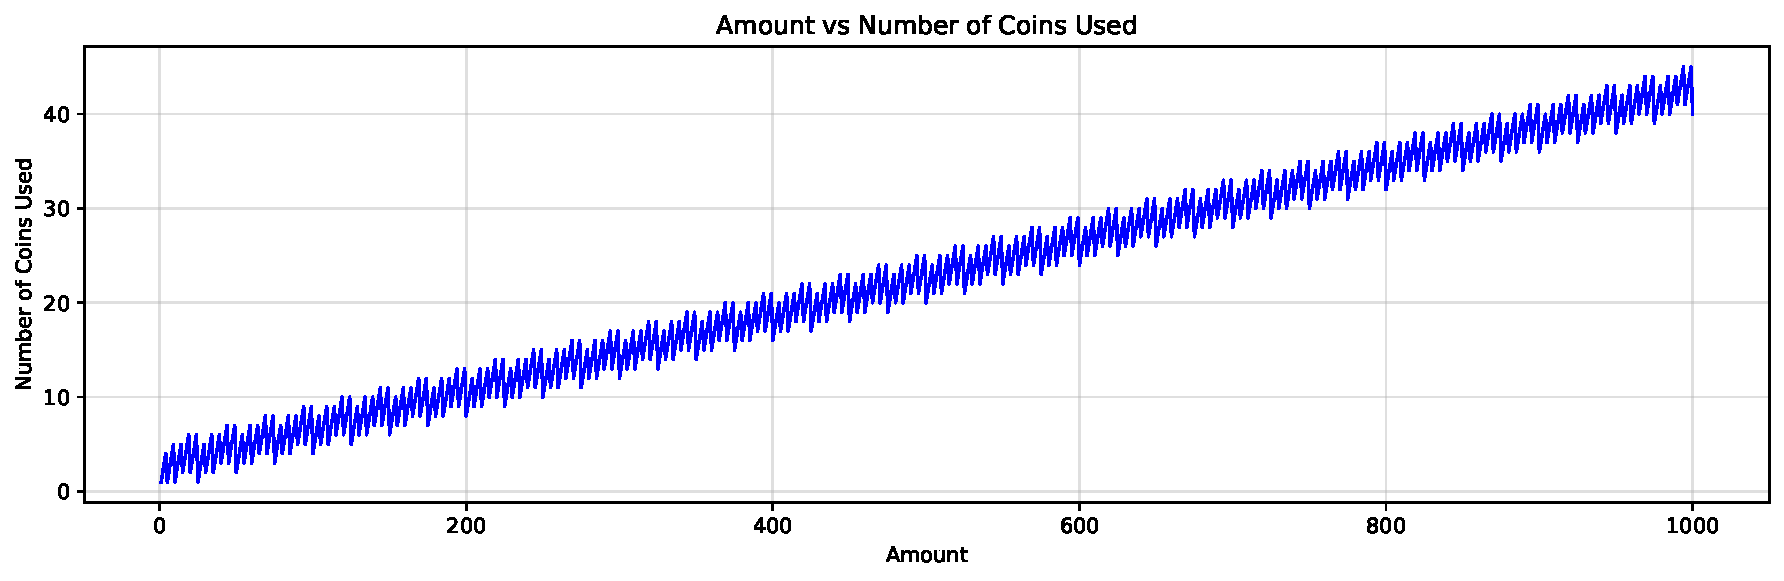
\includegraphics[width=\textwidth]{graphs/greedy_coins_standard_plot.pdf}
  \caption{Number of coins used by the Greedy algorithm for the US coin system (denominations [1, 5, 10, 25]).}
  \label{fig:greedy_coins_standard_plot}
\end{figure}

The above figure shows the relationship between the target amount and the number of coins selected by the Greedy algorithm for the standard US coin system. As expected, the number of coins increases approximately linearly with the target value, while the step-like structure arises from denomination thresholds. Since the US coin system is canonical, the Greedy algorithm always produces the optimal (minimum-coin) result for every target.

\begin{figure}[H]
  \centering
  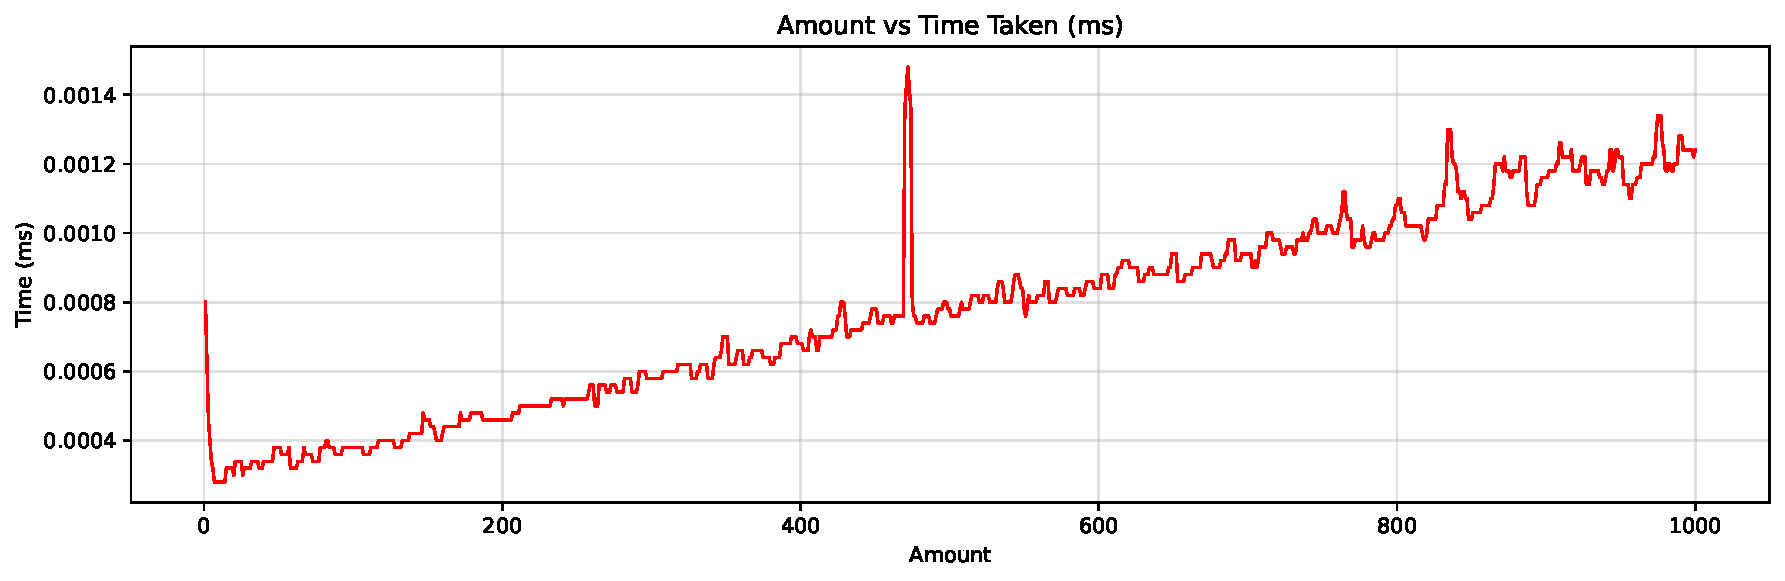
\includegraphics[width=\textwidth]{graphs/greedy_time_standard_plot.pdf}
  \caption{Execution time of the Greedy algorithm for the US coin system.}
  \label{fig:greedy_time_standard_plot}
\end{figure}

Figure~\ref{fig:greedy_time_standard_plot} illustrates the execution time of the same algorithm across the same target range. The runtime remains nearly constant per target due to the direct, iterative nature of the Greedy approach.

\begin{tcolorbox}[colback=gray!5!white, colframe=black, title=Note on Data Smoothing and Filtering]
To improve the readability of the runtime plots, the raw timing data from both the Greedy and Dynamic Programming algorithms was lightly processed before visualization. Real-world execution times often contain random spikes caused by factors such as operating system scheduling, cache misses, and background processes, which can obscure the general performance trend.  

To mitigate these effects, outliers beyond the 1\textsuperscript{st} and 99\textsuperscript{th} percentiles were clipped, and a 7-point rolling median filter was then applied. This smoothing preserves the true computational behavior of the algorithms while removing noise, allowing the plotted curves to more clearly reflect their expected time complexity.
\end{tcolorbox}

Both the \textit{Amount vs. Time} and \textit{Amount vs. Minimum Number of Coins} graphs exhibited the expected linear growth with increasing target values. As the target amount increased, the number of coins required grew proportionally, reflecting the additive nature of the coin combination process. Similarly, the computation time scaled linearly with the target, as each additional value required a fixed and predictable amount of processing. This behavior confirms the theoretical time and space efficiency of the implemented algorithms for canonical coin systems.\\

The observed linear relationship between the target amount and both runtime and coin count remains consistent across other canonical coin systems as well. In the following examples—such as the Binary, Decimal, and Counting systems—the Greedy algorithm continues to yield optimal solutions, demonstrating its correctness and efficiency whenever the denomination set satisfies the canonical property. These cases collectively reinforce the theoretical guarantee that, for canonical coin systems, the Greedy method performs equivalently to the Dynamic Programming approach in both accuracy and asymptotic behavior.\\

\subsection{Canonical Examples}
After observing the linear growth patterns in the standard US coin system, we extend the analysis to other \textbf{canonical coin systems} that also guarantee optimal results under the greedy approach. Each case considers target values ranging from \textbf{1 to 1000}, and we analyze the performance of the greedy algorithm in terms of \textbf{minimum coins used} and \textbf{execution time} for increasing amounts.\\

\begin{itemize}
  \item \textbf{Binary Coin System (1, 2, 4, 8, 16, 32)}\\
  This system represents denominations as powers of two. Since each higher denomination is double the previous one, the greedy algorithm always produces the optimal solution. The following graphs show the number of coins used and execution time for targets 1--512. \\
  \begin{figure}[H]
    \centering
    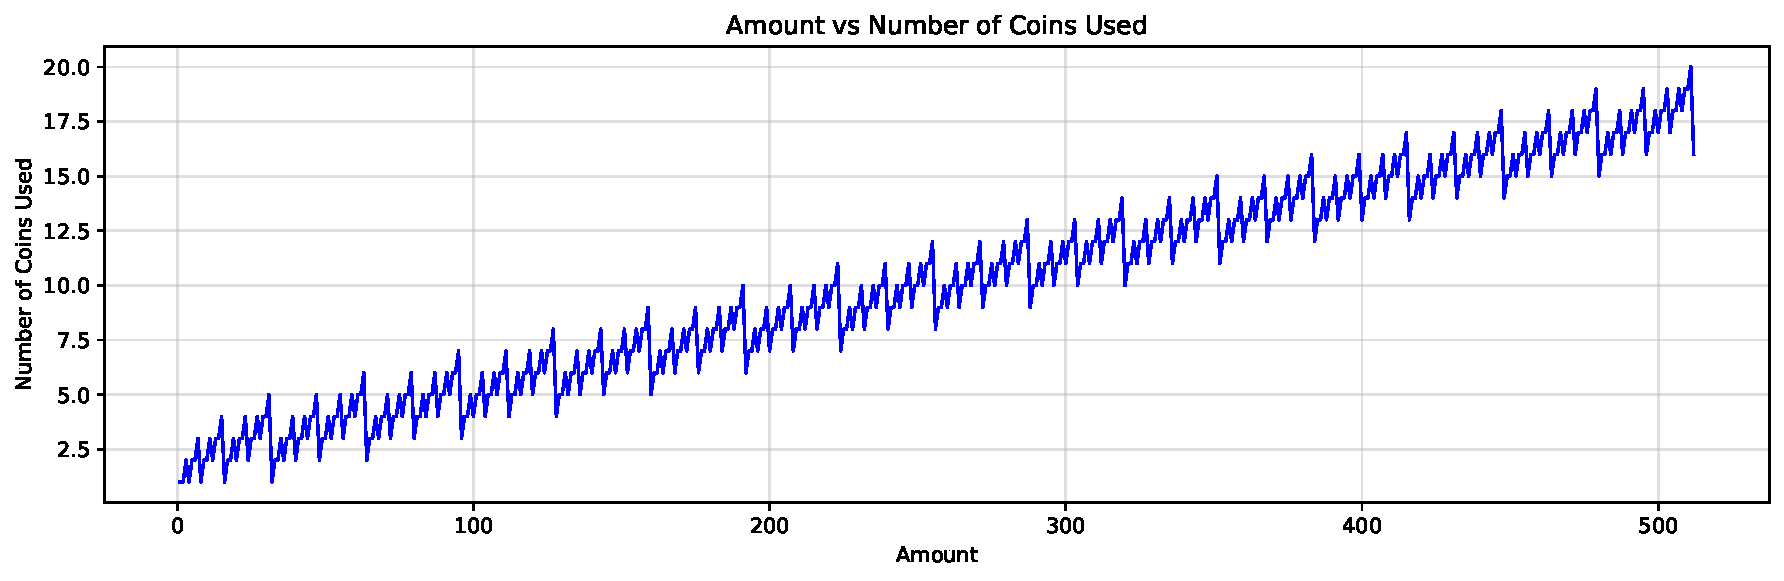
\includegraphics[width=\textwidth]{graphs/greedy_coins_binary_plot.pdf}
    \caption{Greedy algorithm coin comparison for the Binary system (denominations [1, 2, 4, 8, 16, 32]) over targets 1--512.}
    \label{fig:greedy_coins_binary_plot}
  \end{figure}

  \begin{figure}[H]
    \centering
    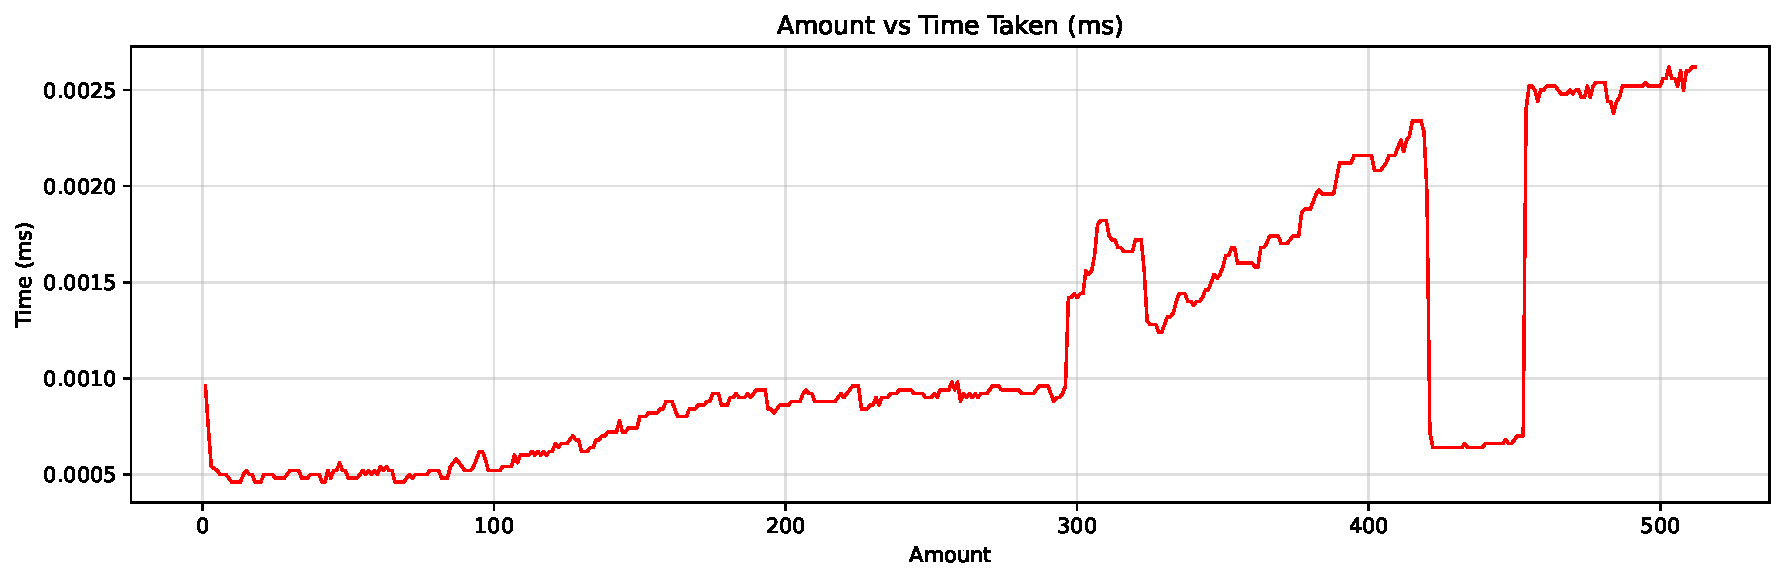
\includegraphics[width=\textwidth]{graphs/greedy_time_binary_plot.pdf}
    \caption{Greedy algorithm time comparison for the Binary system (denominations [1, 2, 4, 8, 16, 32]) over targets 1--512.}
    \label{fig:greedy_time_binary_plot}
  \end{figure}

  \item \textbf{Decimal Coin System (1, 10, 100)}\\
  A base-10 analogue of the binary case. Each denomination is a multiple of 10, ensuring greedy optimality. Targets from 1 to 1000 again show a linear increase in the number of coins and a near-constant computation time.  
  \begin{figure}[H]
    \centering
    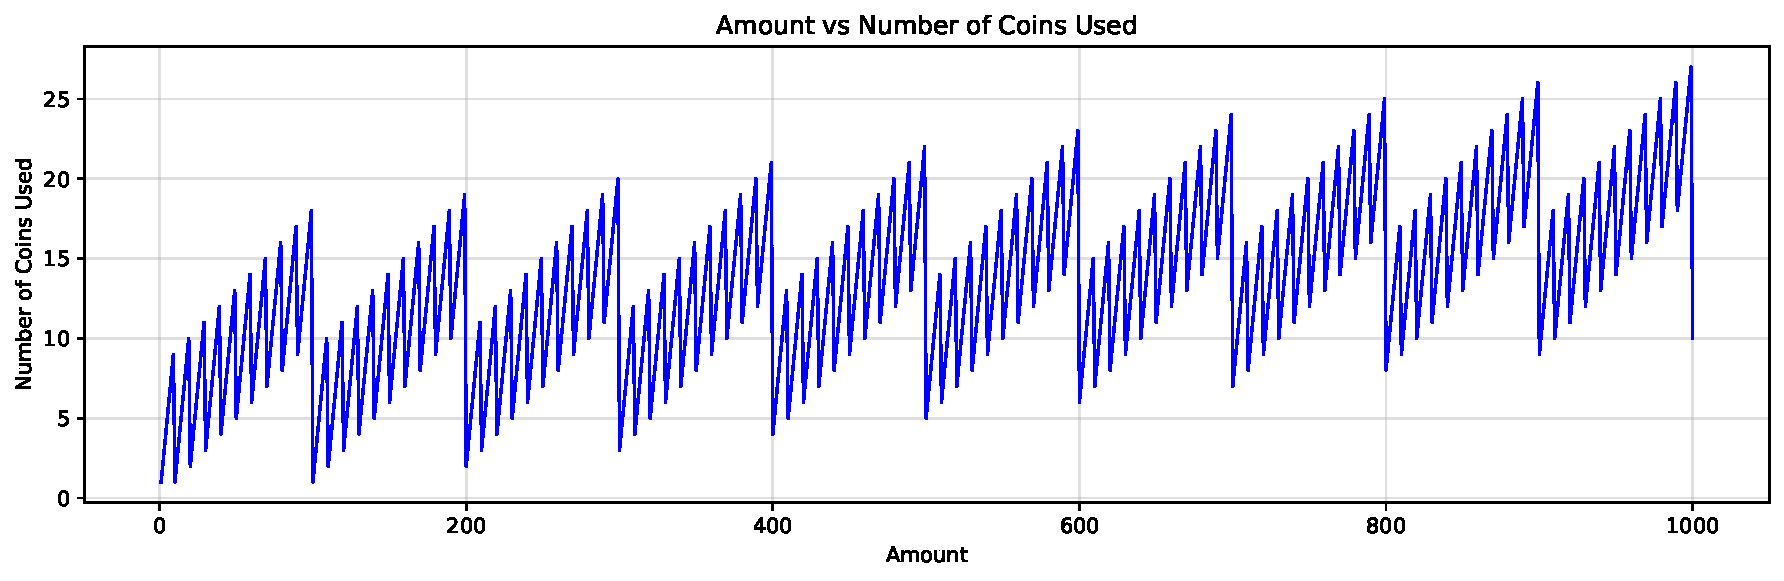
\includegraphics[width=\textwidth]{graphs/greedy_coins_decimal_plot.pdf}
    \caption{Greedy algorithm coin comparison for the Decimal system (denominations [1, 10, 100]) over targets 1--1000.}
    \label{fig:greedy_coins_decimal_plot}
  \end{figure}
  \begin{figure}[H]
    \centering
    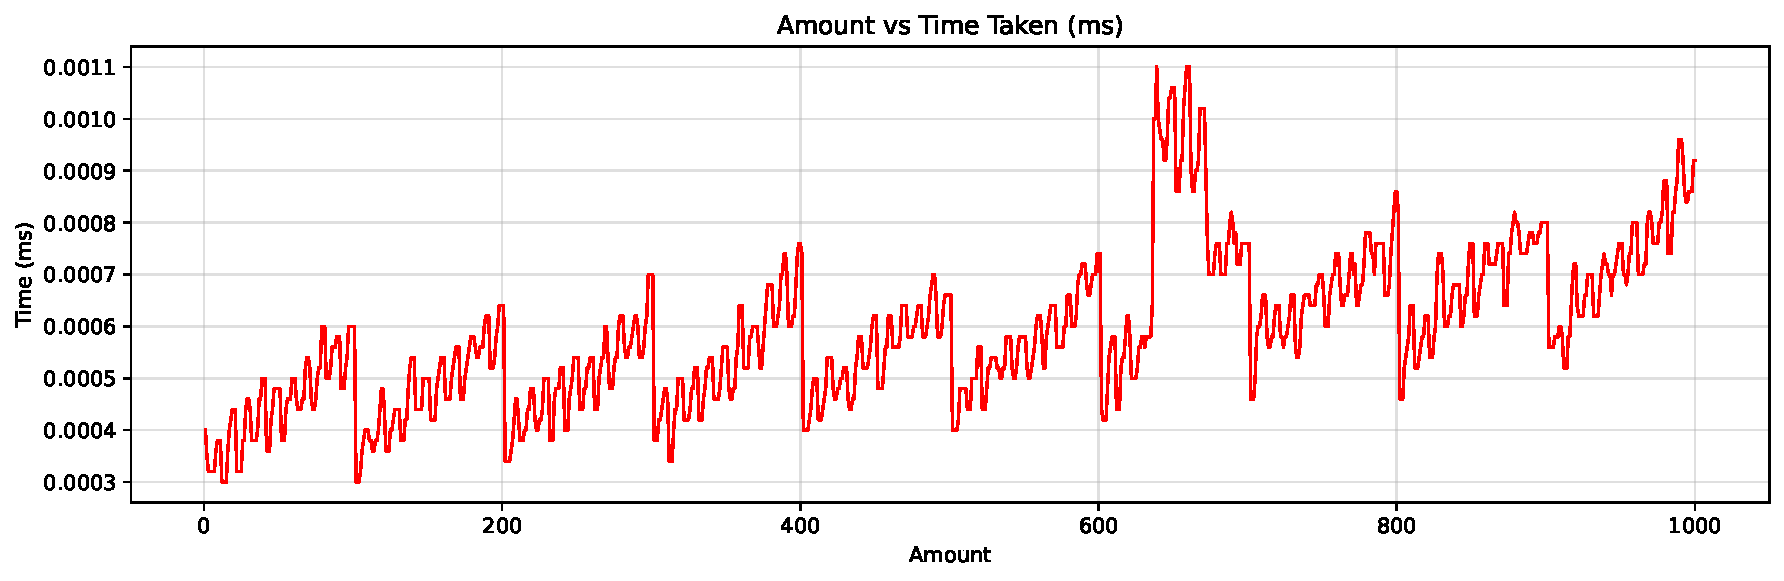
\includegraphics[width=\textwidth]{graphs/greedy_time_decimal_plot.pdf}
    \caption{Greedy algorithm time comparison for the Decimal system (denominations [1, 10, 100]) over targets 1--1000.}
    \label{fig:greedy_time_decimal_plot}
  \end{figure}

  \item \textbf{Counting Coin System (1, 2, 3, 4, 5, 6, 7)}\\
  This simple increasing system mimics counting numbers. The greedy algorithm performs optimally as every denomination divides the next one. Both graphs again display the expected linear growth in coin count and a small, consistent time complexity across all target values.  
  \begin{figure}[H]
    \centering
    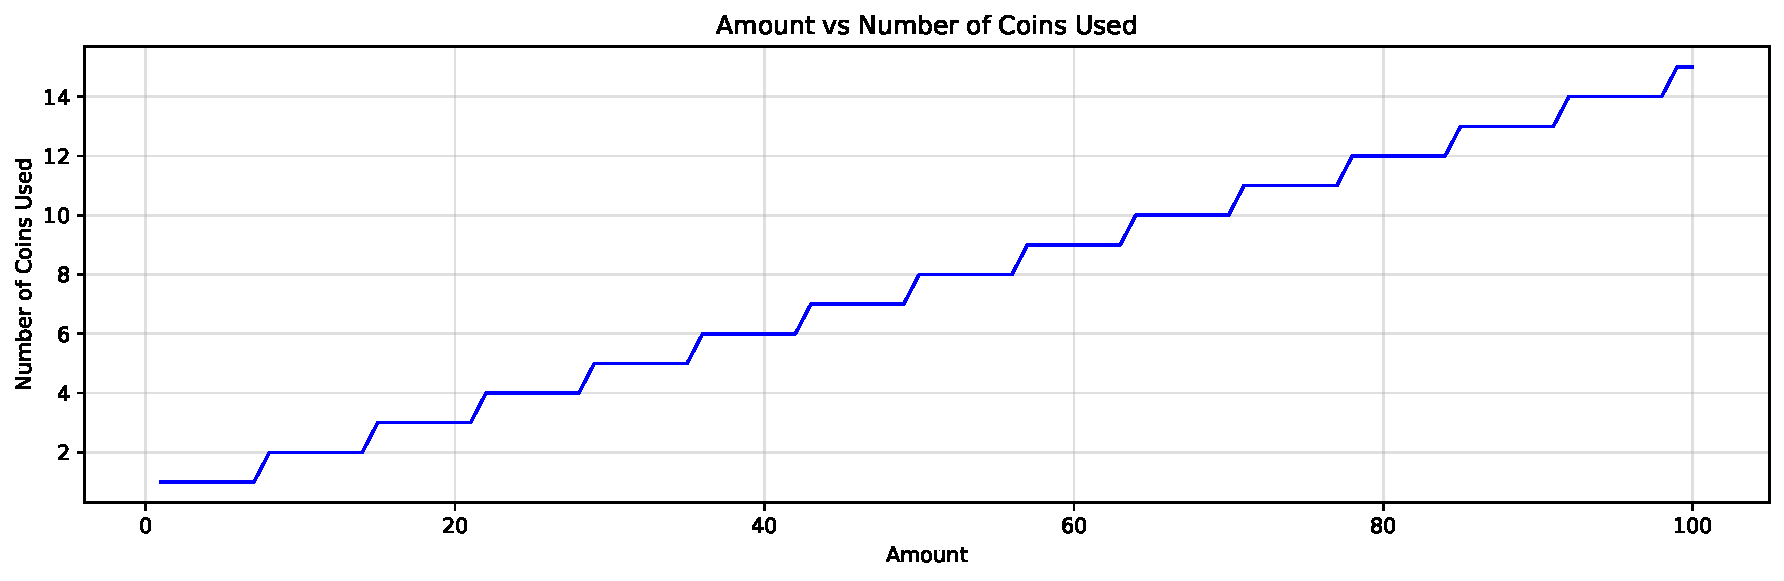
\includegraphics[width=\textwidth]{graphs/greedy_coins_counting_plot.pdf}
    \caption{Greedy algorithm coin comparison for the Counting system (denominations [1, 2, 3, 4, 5, 6, 7]) over targets 1--100.}
    \label{fig:greedy_coins_counting_plot}
  \end{figure}
  \begin{figure}[H]
    \centering
    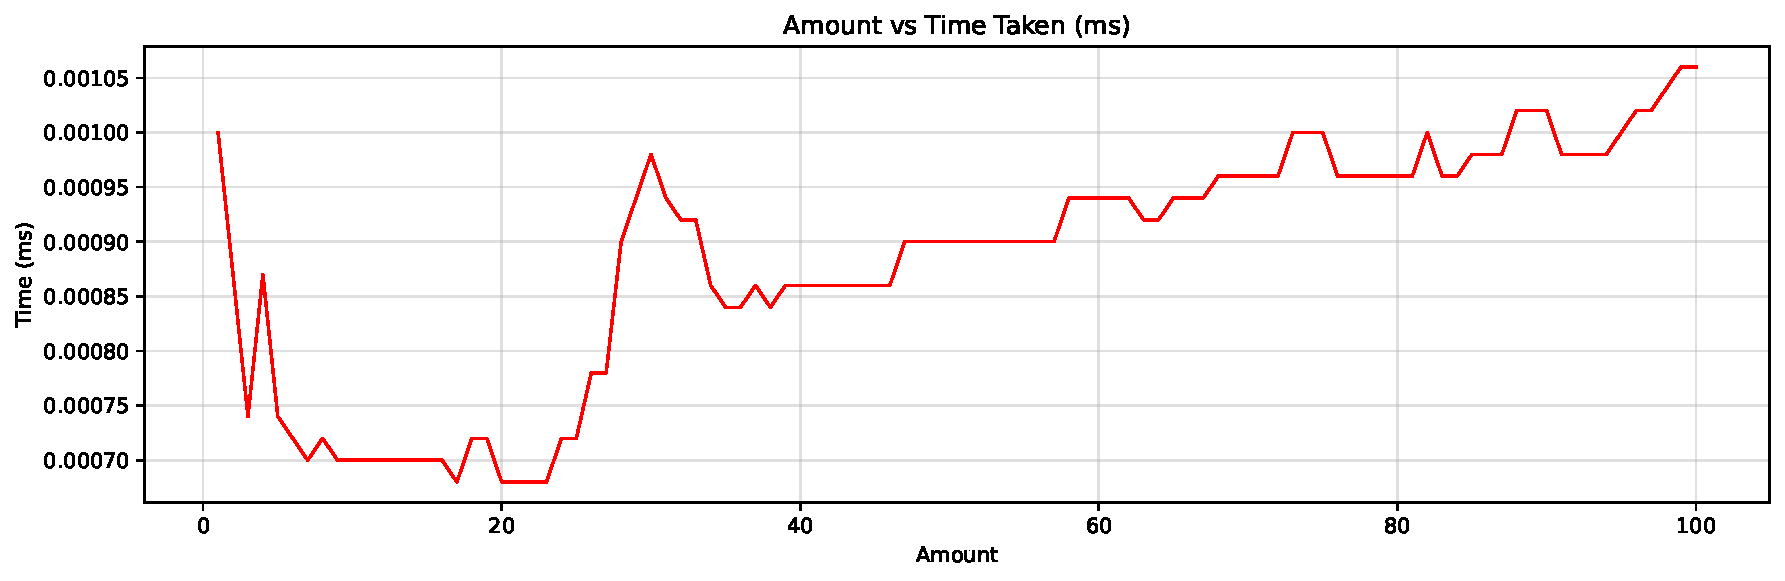
\includegraphics[width=\textwidth]{graphs/greedy_time_counting_plot.pdf}
    \caption{Greedy algorithm time comparison for the Counting system (denominations [1, 2, 3, 4, 5, 6, 7]) over targets 1--100.}
    \label{fig:greedy_time_counting_plot}
  \end{figure}
\end{itemize}

\subsection{Non-Canonical Example}
\noindent
While the greedy algorithm performs optimally for canonical coin systems, it can fail for certain \textbf{non-canonical systems}, where the largest-coin-first strategy does not always yield the minimum number of coins. To illustrate this, consider the following small examples:

\begin{itemize}
    \item \textbf{Example 1:} Denominations [1, 3, 4], Target = 6.  
    Greedy selects 4 + 1 + 1 = 3 coins, whereas the optimal solution is 3 + 3 = 2 coins.

    \item \textbf{Example 2:} Denominations [1, 5, 7], Target = 10.  
    Greedy selects 7 + 1 + 1 + 1 = 4 coins, whereas the optimal solution is 5 + 5 = 2 coins.

    \item \textbf{Example 3:} Denominations [1, 9, 10], Target = 18.  
    Greedy selects 10 + 1 + 1 + 1 + 1 + 1 + 1 + 1 + 1 + 1 = 10 coins, whereas the optimal solution is 9 + 9 = 2 coins.
\end{itemize}

\noindent
These examples motivate the study of \textbf{non-canonical coin systems} in our experiments. In the following sections, we present the datasets and graphs for several such non-canonical systems, comparing the performance of the greedy and dynamic programming algorithms across a range of target amounts.\\

\noindent
After studying canonical coin systems where the Greedy algorithm reliably produces optimal solutions, we now examine \textbf{non-canonical coin systems}. In these systems, the simple largest-coin-first strategy can fail to minimize the number of coins, highlighting the limitations of the Greedy approach. Analyzing non-canonical systems motivates the use of more robust methods, such as Dynamic Programming, to guarantee minimum coin counts across all target values.

\noindent
One notable non-canonical example is the \textbf{Old Indian Coin System (in paise)}, which consists of the denominations [1, 2, 5, 10, 20, 25, 50]. Unlike canonical systems, this set includes coins that do not satisfy the divisibility conditions required for Greedy optimality. Consequently, there exist target amounts where the Greedy algorithm does not yield the minimum number of coins. In the following sections, we analyze the performance of the Greedy algorithm on this system in terms of both coin counts and execution time, and later compare it with the Dynamic Programming approach to demonstrate the correct minimum-coin solutions.

\begin{tcolorbox}[colback=gray!5!white, colframe=black, title=Note on using DP without introducing it]
We will use DP algorithm for some of our next graph to compare and show the non-canonicity of the chosen coin denomination, We will show the optimality of DP in our next chapter with pseducode and python implementation with many examples using canonical and non-canonical coin denomination.
\end{tcolorbox}

\begin{itemize}
    \item \textbf{Old Indian Coin System (1, 2, 5, 10, 20, 25, 50) paise}\\
    This historical coin system contains denominations that are not strictly multiples of each other, making it \textbf{non-canonical}. For example, to make a target of 30, the greedy algorithm will select 25 + 5 = 2 coins, which is optimal, but for some targets such as 40, it will select 25 + 10 + 5 = 3 coins, whereas the true minimum is 20 + 20 = 2 coins.  
    \begin{figure}[H]
      \centering
      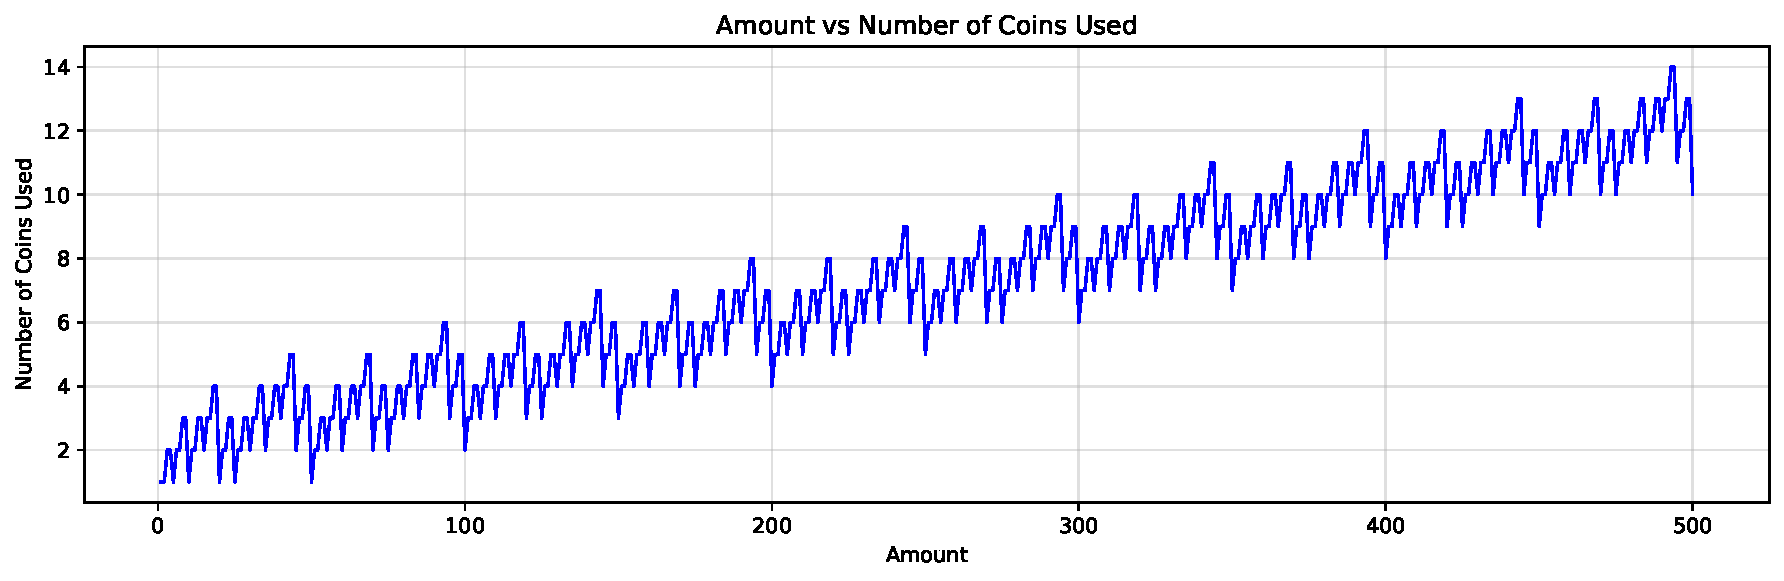
\includegraphics[width=\textwidth]{graphs/greedy_coins_indiancoinsystum_plot.pdf}
      \caption{Number of coins used by the Greedy algorithm for the Old Indian Coin System (denominations [1, 2, 5, 10, 20, 25, 50]).}
      \label{fig:greedy_coins_indiancoinsystum_plot}
    \end{figure}
    The above figure illustrates the number of coins used by the Greedy algorithm for the Old Indian Coin System (denominations [1, 2, 5, 10, 20, 25, 50]). It highlights how the greedy choice selects coins for increasing target amounts, showing linear growth with occasional deviations from the minimum for certain targets.

    \begin{figure}[H]
      \centering
      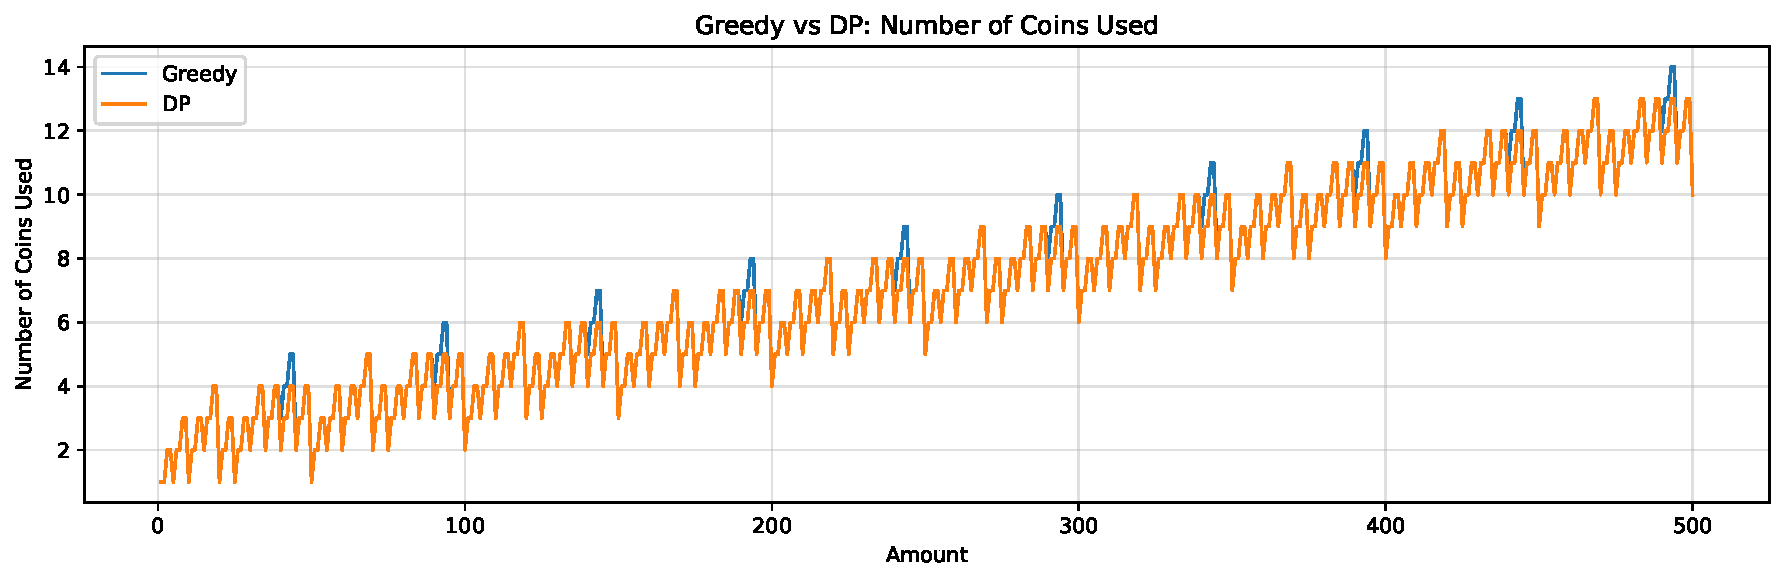
\includegraphics[width=\textwidth]{graphs/compare_coins_indiancoinsystum_plot.pdf}
      \caption{Comparison of minimum coins used by the Greedy and Dynamic Programming algorithms for the Old Indian Coin System over targets 1--500.}
      \label{fig:compare_coins_indiancoinsystum_plot}
    \end{figure}

    The comparison graph above shows where the Greedy algorithm aligns with Dynamic Programming and where it fails to yield the minimum number of coins. Deviations indicate non-canonical behavior in this historical coin system, emphasizing the need for Dynamic Programming to guarantee correctness.

    \begin{figure}[H]
      \centering
      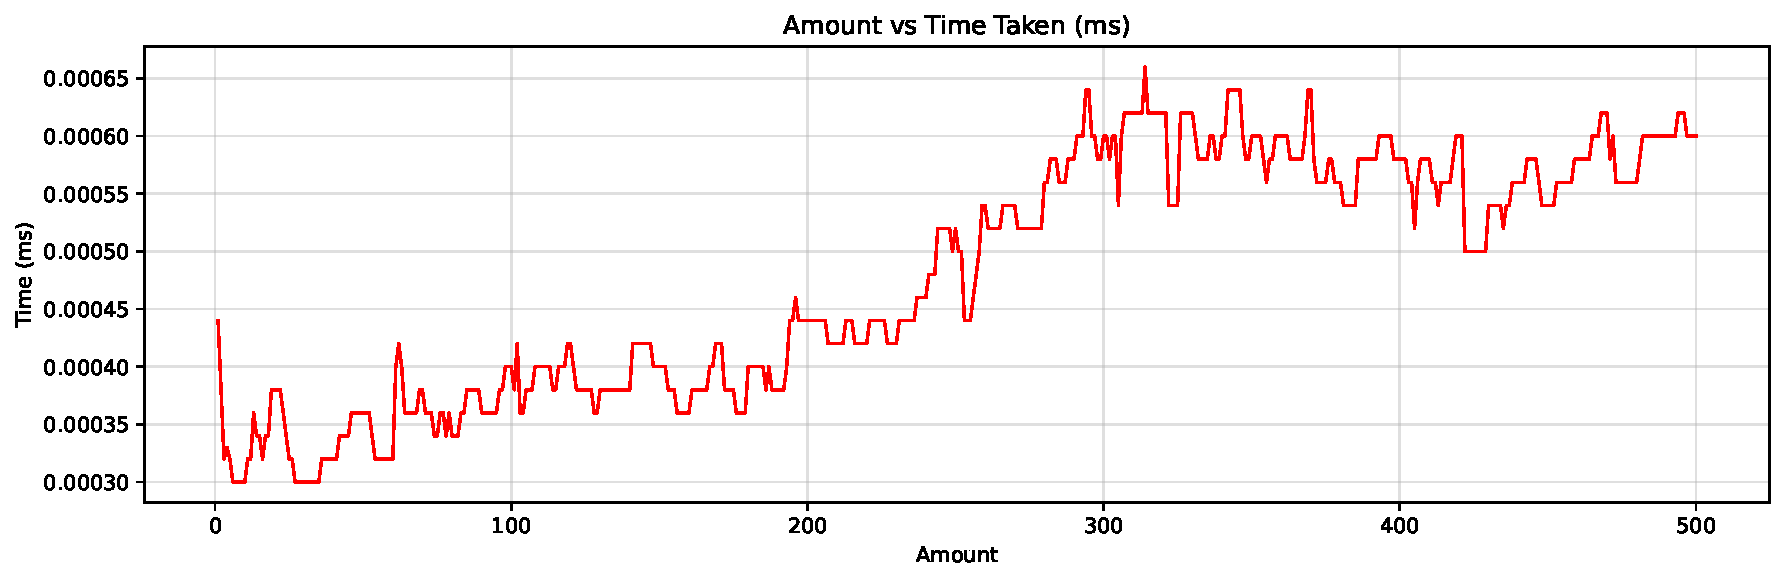
\includegraphics[width=\textwidth]{graphs/greedy_time_indiancoinsystum_plot.pdf}
      \caption{Execution time of the Greedy algorithm for the Indian Coin System before 1800.}
      \label{fig:greedy_time_indiancoinsystum_plot}
    \end{figure}

    \item \textbf{Square Coin System (1, 4, 9, 16, 25, 36, 49)}\\
    This system uses denominations that are perfect squares. It is non-canonical, and the greedy algorithm may fail for certain targets. For example, to make 18, greedy selects 16 + 1 + 1 = 3 coins, while the optimal solution is 9 + 9 = 2 coins.  
    \begin{figure}[H]
      \centering
      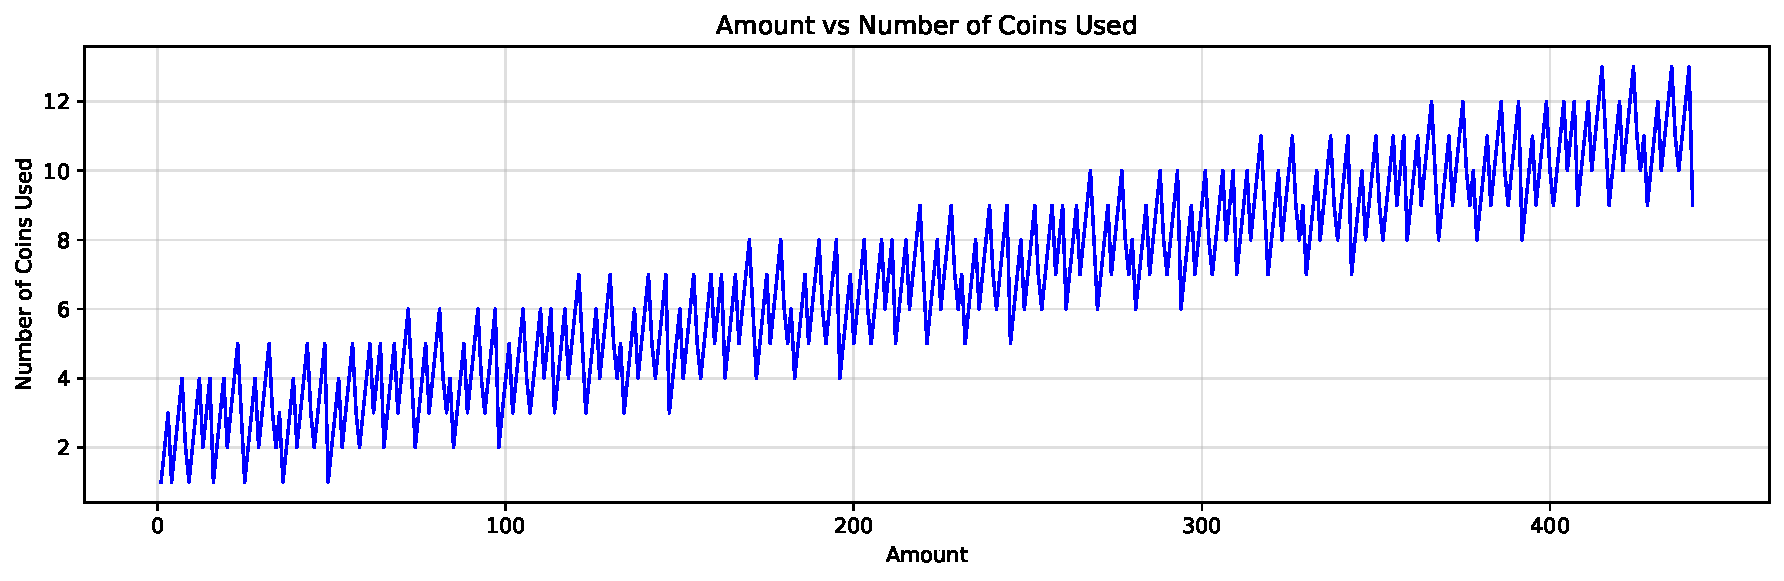
\includegraphics[width=\textwidth]{graphs/greedy_coins_square_plot.pdf}
      \caption{Number of coins used by the Greedy algorithm for the Square coin system (denominations [1, 4, 9, 16, 25, 36, 49]).}
      \label{fig:greedy_coins_square_plot}
    \end{figure}

    The above figure illustrates the number of coins used by the Greedy algorithm for the Square Coin System (denominations [1, 4, 9, 16, 25, 36, 49]). Linear growth is observed in most targets, but for specific values, the Greedy choice selects suboptimal coins

    \begin{figure}[H]
      \centering
      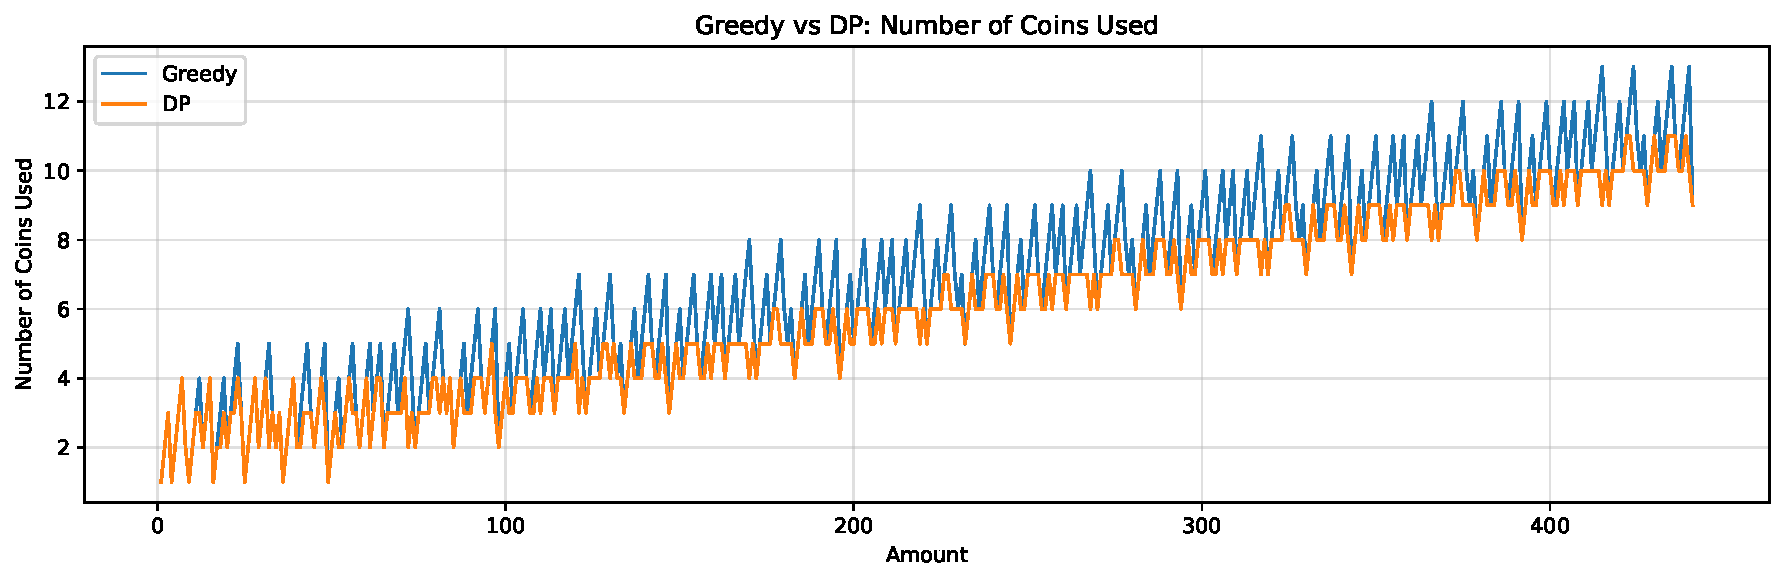
\includegraphics[width=\textwidth]{graphs/compare_coins_square_plot.pdf}
      \caption{Comparison of minimum coins used by the Greedy and Dynamic Programming algorithms for the Square Coin System over targets 1--441.}
      \label{fig:compare_coins_square_plot}
    \end{figure}

    The comparison graph demonstrates the failure points of the Greedy algorithm. While Dynamic Programming consistently provides the minimum number of coins, the Greedy algorithm sometimes overestimates, highlighting the limitations of non-canonical denominations.

    \begin{figure}[H]
      \centering
      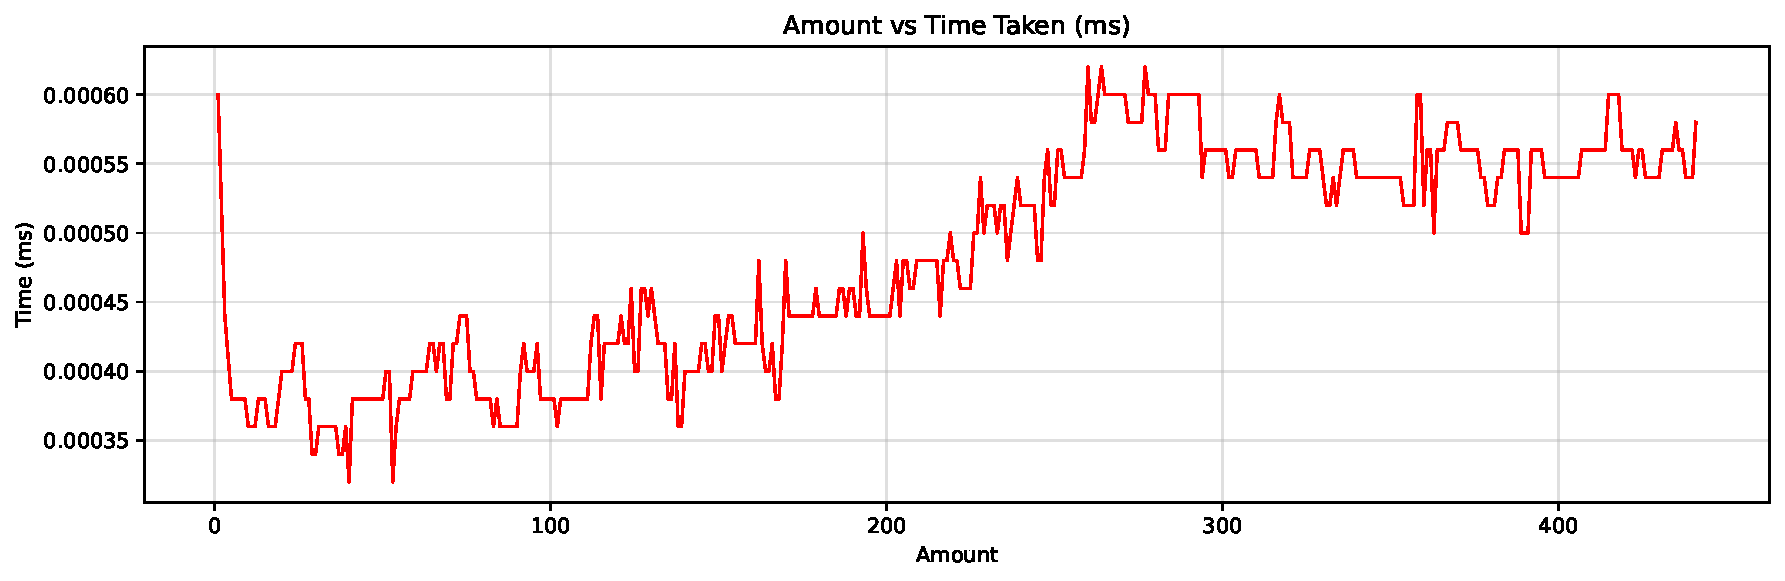
\includegraphics[width=\textwidth]{graphs/greedy_time_square_plot.pdf}
      \caption{Execution time of the Greedy algorithm for the Square coin system.}
      \label{fig:greedy_time_square_plot}
    \end{figure}

    \item \textbf{Twin Prime Coin System (1, 41, 43, 101, 103)}\\
    This system uses coin denominations based on twin primes. Non-canonical behavior is frequent, and greedy may not be optimal. For example, to make 84, greedy selects 43 + 41 = 2 coins, which is optimal, but for 83, greedy will select one 43-coin and forty 1-coins = 41 coins, whereas the true minimum could be 41 + 41 + 1 = 3 coins, illustrating inconsistencies.  
    \begin{figure}[H]
      \centering
      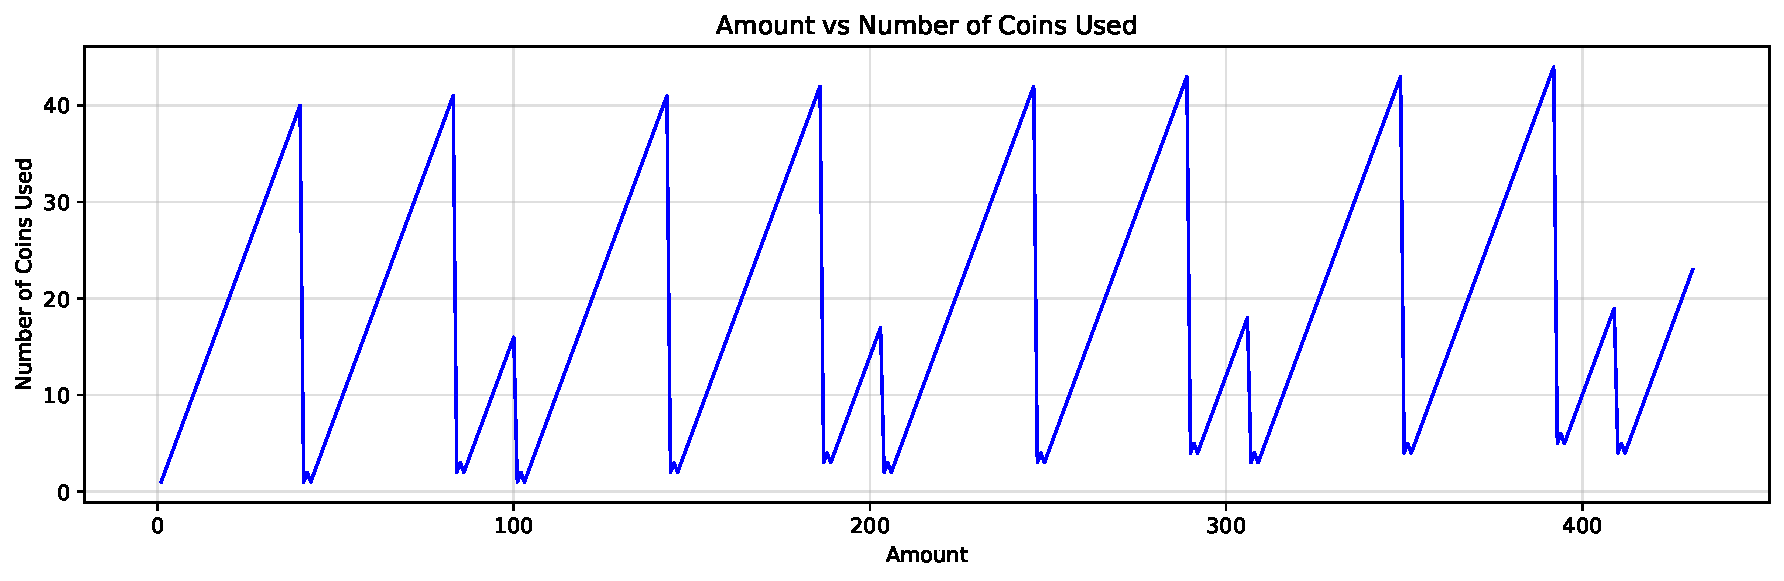
\includegraphics[width=\textwidth]{graphs/greedy_coins_twin_prime_plot.pdf}
      \caption{Number of coins used by the Greedy algorithm for the Twin Prime coin system (denominations [1, 41, 43, 101, 103]).}
      \label{fig:greedy_coins_twin_prime_plot}
    \end{figure}

    The above figure illustrates the number of coins used by the Greedy algorithm for the Twin Prime Coin System (denominations [1, 41, 43, 101, 103]). Although linear patterns appear for some targets, specific amounts cause the Greedy algorithm to select a higher number of coins than necessary.

    \begin{figure}[H]
      \centering
      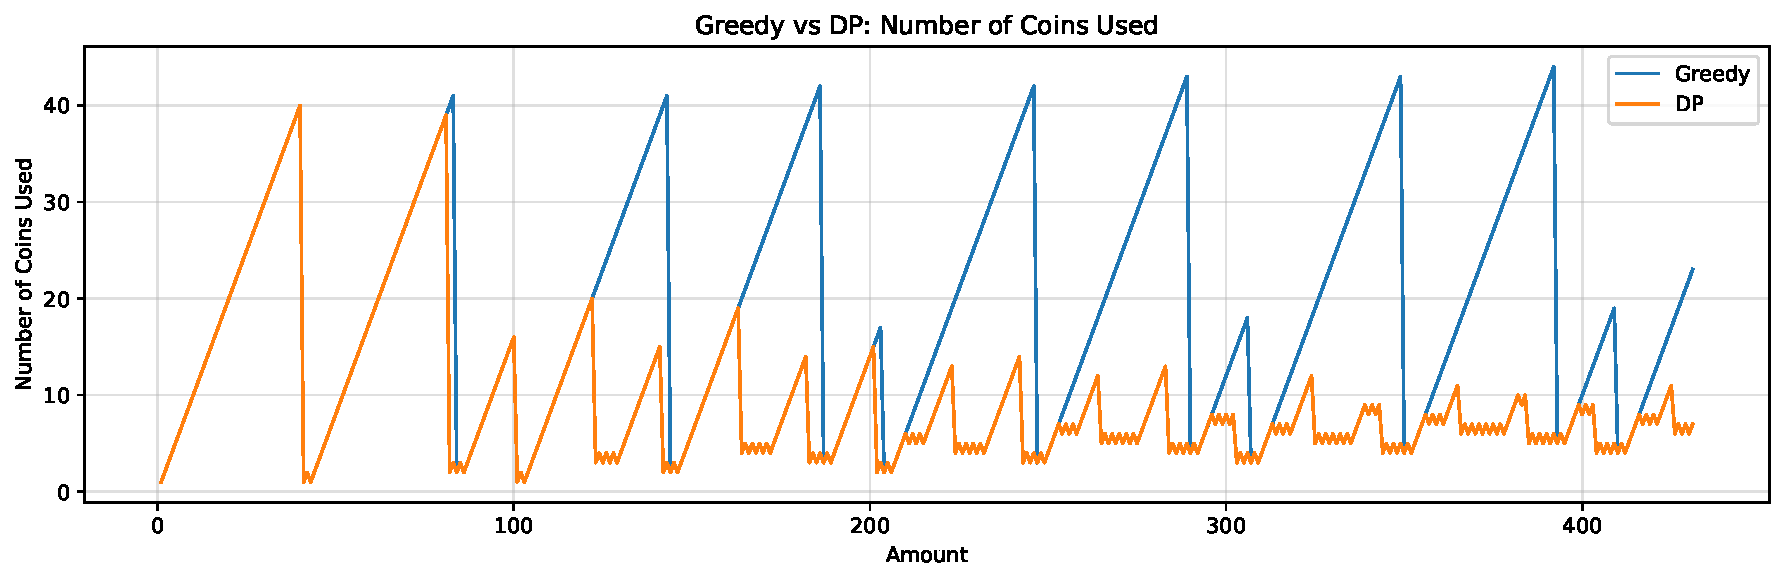
\includegraphics[width=\textwidth]{graphs/compare_coins_twin_prime_plot.pdf}
      \caption{Comparison of minimum coins used by the Greedy and Dynamic Programming algorithms for the Twin Prime Coin System over targets 1--431.}
      \label{fig:compare_coins_twin_prime_plot}
    \end{figure}

    The comparison graph highlights targets where the Greedy algorithm fails. Dynamic Programming provides the correct minimum coin count, clearly showing the advantage of using a robust algorithm for non-canonical systems.

    \begin{figure}[H]
      \centering
      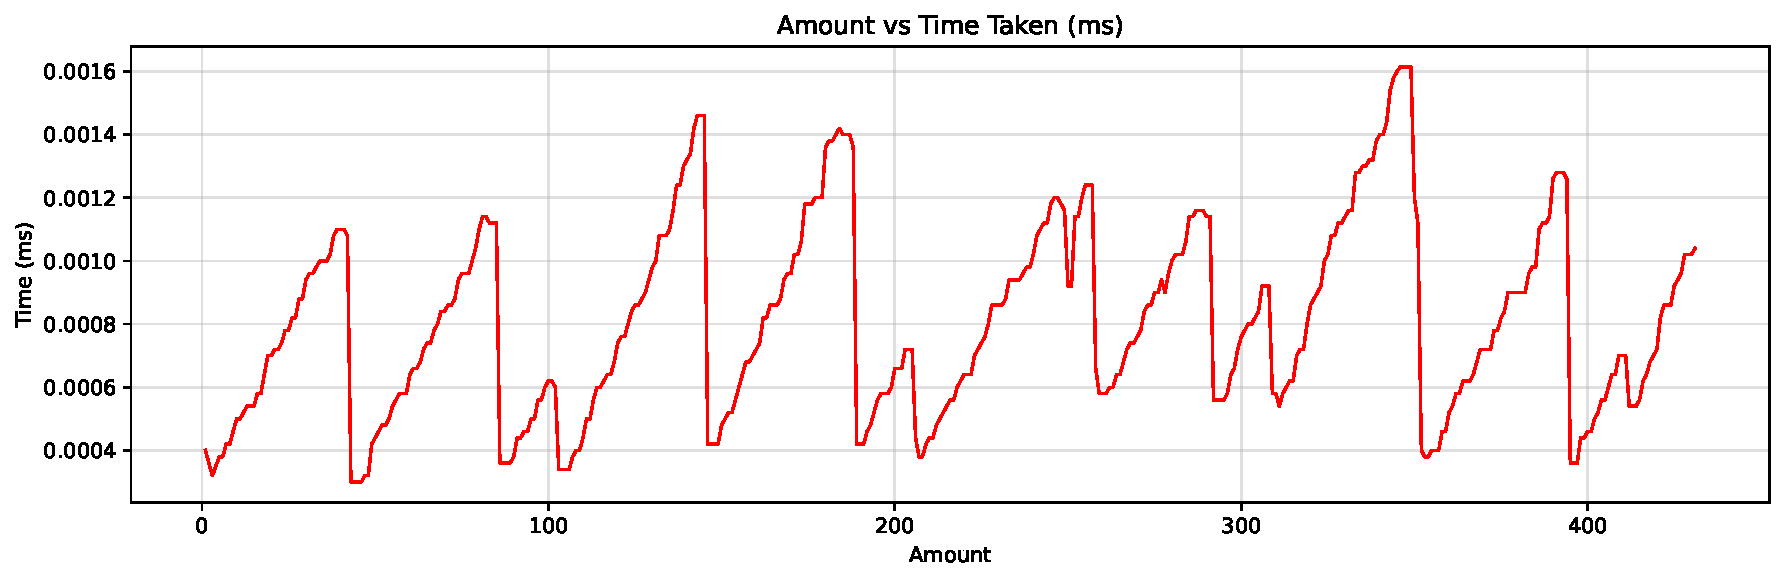
\includegraphics[width=\textwidth]{graphs/greedy_time_twin_prime_plot.pdf}
      \caption{Execution time of the Greedy algorithm for the Twin Prime coin system.}
      \label{fig:greedy_time_twin_prime_plot}
    \end{figure}


\item \textbf{Meme Number Coin System (1, 6, 7, 69, 420)}\\
This system uses coin denominations inspired by well-known internet meme numbers. The denominations are irregular and non-canonical, meaning that the greedy algorithm does not always yield the optimal (minimum coin) solution. Nonlinearities and discontinuities in the coin selection pattern frequently appear.

For example, to make the value 12, the greedy algorithm would choose one 7-coin and five 1-coins (total 6 coins). However, the true minimum is achieved using two 6-coins, demonstrating how greedy fails under non-canonical ratios.

\begin{figure}[H]
  \centering
  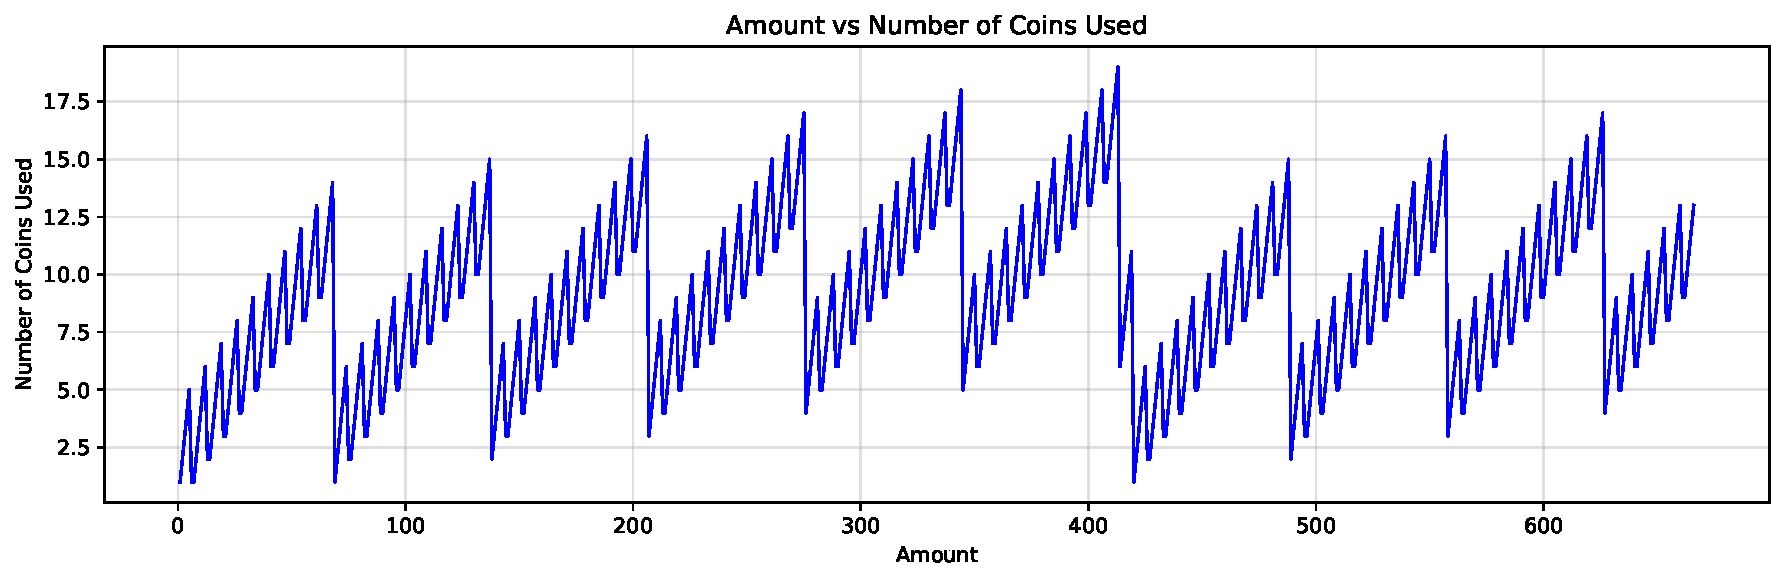
\includegraphics[width=\textwidth]{graphs/greedy_coins_meme_plot.pdf}
  \caption{Number of coins used by the Greedy algorithm for the Meme Number Coin System (denominations [1, 6, 7, 69, 420]).}
  \label{fig:greedy_coins_meme_number_plot}
\end{figure}

The above figure shows the number of coins used by the Greedy algorithm across targets from 1 to 666. While smooth linear segments can be observed for smaller targets, sharp spikes occur at specific values where the greedy choice produces suboptimal results.

\begin{figure}[H]
  \centering
  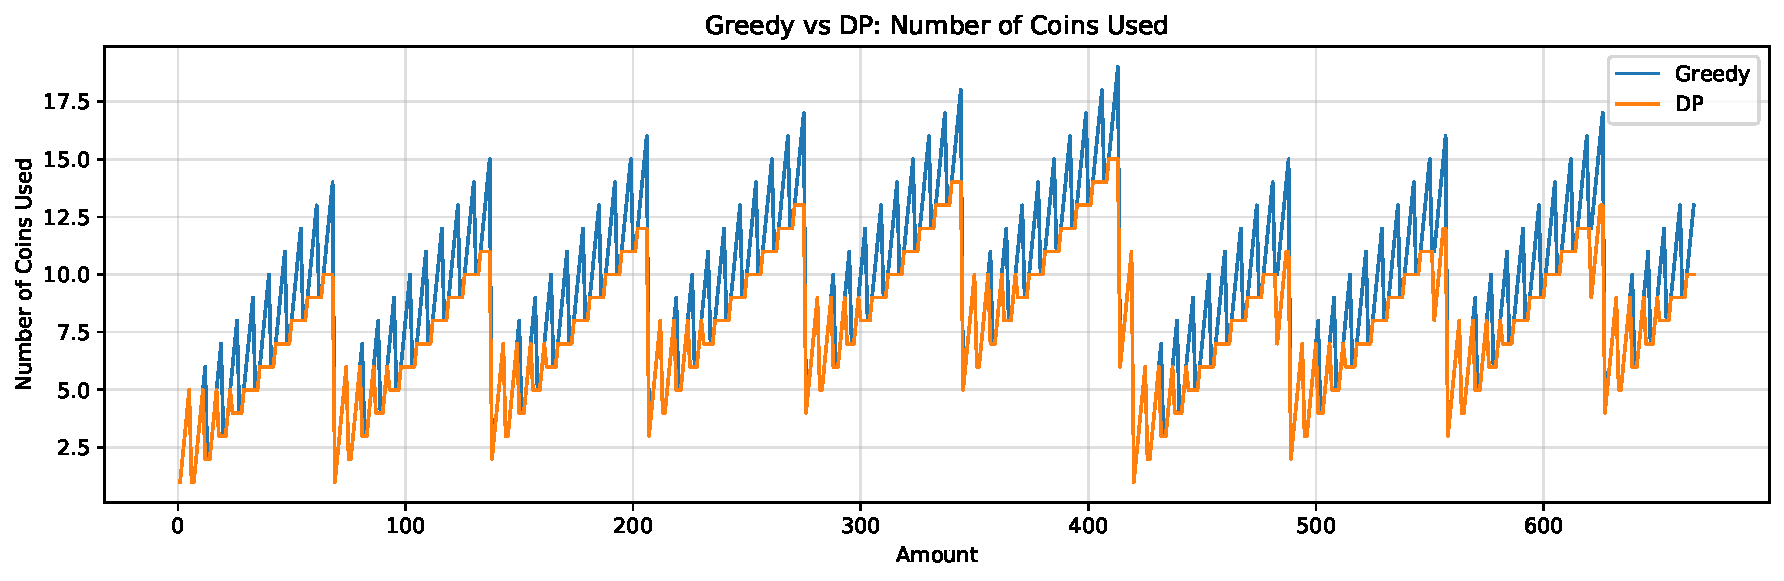
\includegraphics[width=\textwidth]{graphs/compare_coins_meme_plot.pdf}
  \caption{Comparison of minimum coins used by the Greedy and Dynamic Programming algorithms for the Meme Number Coin System over targets 1--666.}
  \label{fig:compare_coins_meme_number_plot}
\end{figure}

The comparison highlights the numerous instances where the greedy algorithm diverges from the optimal coin count obtained via Dynamic Programming. The DP algorithm systematically explores all combinations, identifying configurations where small denominations can outperform a single large denomination, particularly in irregular systems like this one.

\begin{figure}[H]
  \centering
  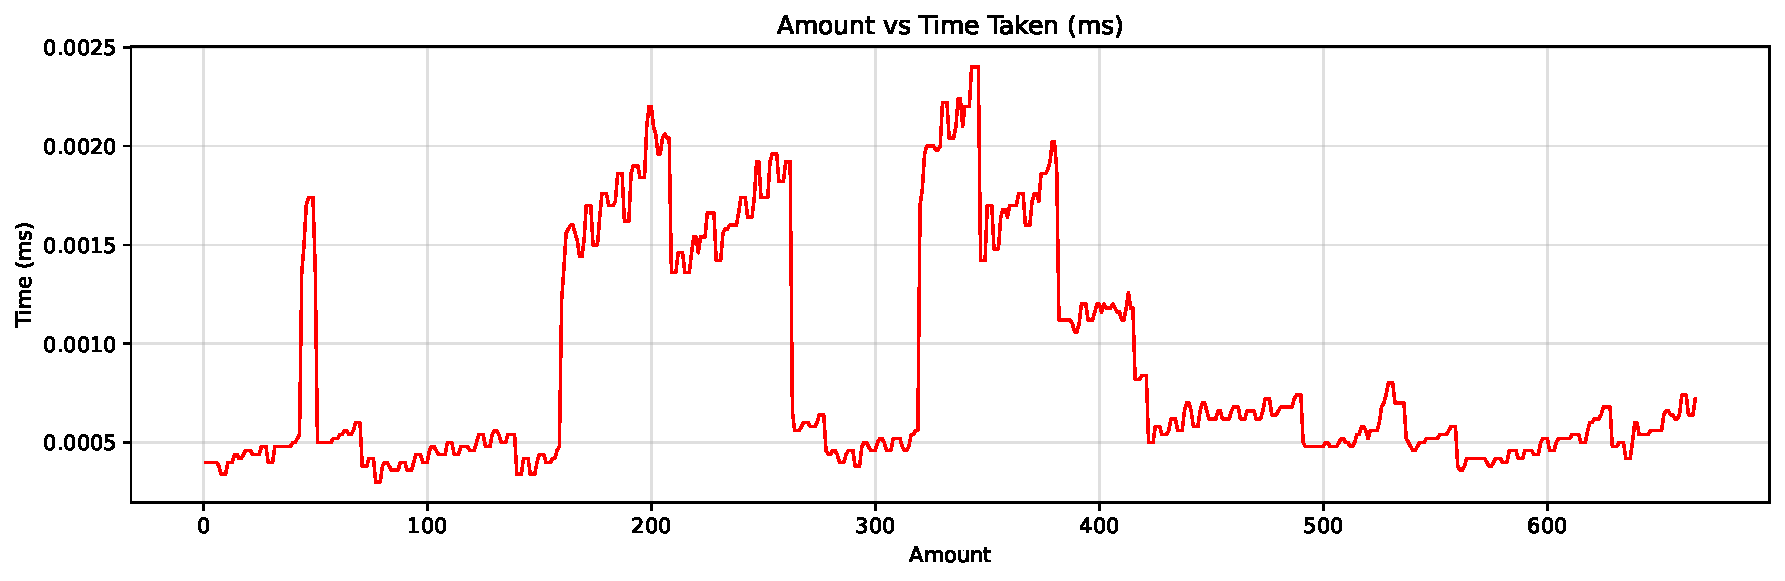
\includegraphics[width=\textwidth]{graphs/greedy_time_meme_plot.pdf}
  \caption{Execution time of the Greedy algorithm for the Meme Number Coin System.}
  \label{fig:greedy_time_meme_number_plot}
\end{figure}
\end{itemize}

Although the greedy algorithm remains extremely fast, the plot above confirms that speed comes at the expense of optimality in the Meme Number Coin System. This example reinforces that non-canonical coin structures, such as those based on arbitrary or humorous numbers, require more sophisticated algorithms like Dynamic Programming to guarantee minimal coin usage.


\section{Conclusion}
\label{sec:greedy_conclusion}

In this chapter, we studied the Greedy algorithm for the Coin Change problem in detail. We began by defining the problem in the greedy setting (Section~1.1) and presented the corresponding pseudocode (Section~1.2). The proof of correctness (Section~1.3) established that the greedy approach produces optimal results for canonical coin systems, where each denomination is suitably divisible by the larger ones. We analyzed the time and space complexity of the algorithm (Section~1.4), demonstrating its efficiency as a simple, linear-time solution. Section~1.5 provided a Python implementation, and Section~1.6 presented testing results across various coin systems, including canonical examples (Binary, Decimal, Counting, Standard US) and non-canonical examples (Indian Coin System, Square, Twin Prime, Meme).

The experiments confirmed that the Greedy algorithm is fast and accurate for canonical coin systems, consistently producing the minimum number of coins with predictable runtime. However, in non-canonical systems, certain target amounts reveal its limitations, where the greedy choice does not yield the optimal coin count. This motivates the need for more robust methods, such as Dynamic Programming, to guarantee correctness in all cases. Overall, the chapter demonstrates both the strengths and limitations of the Greedy approach and provides a practical framework for implementing and analyzing it in real-world coin systems.


%------------------------------------------------------------------------------------------------------------------------------------------------------------------------------------------------------------------------------------------------------------------------------------------------------------------------------------------------------------------------------------
\chapter{Dynamic Programming for Coin Change \centering}
\section{Why use Dynamic Programming}
\label{sec:dp-algo}
The greedy algorithm is attractive because it is single-pass and runs in $\Theta(n)$ time for $n$ denominations, but its optimality depends on a strong structural property known as \textit{canonicity}. Once the coin system violates this property, the greedy choice (always taking the largest coin that fits) can no longer be trusted. A classic counterexample is the set $\{1, 3, 4\}$ for a target value of $6$: the greedy algorithm produces $4 + 1 + 1$ (three coins), while the optimal solution is $3 + 3$ (two coins). Because this failure occurs silently (no error flag is raised), the algorithm may return a suboptimal answer that propagates into downstream financial calculations. In safety-critical or high-volume payment systems, this behavior is unacceptable.

Dynamic programming (DP) removes this brittleness by construction. It does not rely on any assumed structure of the denomination set; instead, it exhaustively explores every possible decomposition of the target amount into sub-amounts, storing the best solution found so far for each sub-amount in a table. The recurrence
\[
C[i] = \min_{d \in \text{denom}} (1 + C[i - d])
\]
with base case $C[0] = 0$, guarantees that $C[A]$ represents the true minimum number of coins required for amount $A$, regardless of whether the system is canonical, non-canonical, or even pathological (for example, $\{1, 7, 13, 19\}$). Consequently, DP acts as a certifiable fallback: it can be invoked whenever the canonicity status of a coin set is unknown, or when the set is explicitly non-canonical (such as commemorative or token-based currencies).

Although the asymptotic cost rises to $\Theta(nA)$ and the memory footprint to $\Theta(A)$, these overheads are modest for the range of amounts encountered in everyday retail (tens or hundreds of currency units) and are easily bounded in software. Moreover, once the denomination set is fixed, the table can be reused for multiple payments, thereby amortizing the computational cost across transactions. The same table also yields not only the minimum number of coins but also the exact coin multiset, which is valuable for audit trails required by regulators and payment processors.

In summary, dynamic programming is the preferred method when correctness must be unconditional. It trades a small, predictable overhead for the elimination of silent failures, thereby providing a robust and future-proof solution to the coin change problem.

\section{Problem Description: Coin Change Problem}

The coin change problem can be stated formally as follows:

\begin{itemize}
    \item \textbf{Input:} 
    A set of coin denominations
    \[
        D = \{d_1, d_2, \dots, d_k\}, \quad d_1 < d_2 < \cdots < d_k,
    \]
    where each $d_i \in \mathbb{N}$ and typically $d_1 = 1$ to ensure that every amount can be represented. 
    Also, a target value $N \in \mathbb{N}$.

    \item \textbf{Objective:} 
    Find non-negative integers $x_1, x_2, \dots, x_k$ such that
    \[
        \sum_{i=1}^{k} x_i d_i = N
    \]
    and the total number of coins
    \[
        \sum_{i=1}^{k} x_i
    \]
    is minimized.

    \item \textbf{Remarks:} 
    Unlike the greedy algorithm, no specific selection order is imposed. The solution may require combinations that do not always select the largest denomination first. Optimal solutions can be obtained using dynamic programming or integer linear programming.\\
    We will be using dynamic programming to find optimal solution.
\end{itemize}

\newpage

\section{Pseudocode for Coin Change using Dynamic Programming}
\begin{algorithm}
\caption{Dynamic Programming Algorithm for Coin Change}
\begin{algorithmic}[1]
\Procedure{CoinChangeDP}{$coins, target$}
    \State $dp \gets$ array of size $(target + 1)$ with all values $\infty$ 
    \State \Comment{Initialize DP table with infinity}
    \State $dp[0] \gets 0$ \Comment{Zero coins needed to make amount 0}

    \For{$x = 1$ to $target$}
        \For{$coin \in coins$}
            \If{$coin \le x$}
                \State $dp[x] \gets \min(dp[x], dp[x - coin] + 1)$ \Comment{Update min coins}
            \EndIf
        \EndFor
    \EndFor

    \If{$dp[target] \neq \infty$}
        \State \Return $dp[target]$ \Comment{Return min. no. of coins for target}
    \Else
        \State \Return $-1$ \Comment{Amount cannot be formed with given coins}
    \EndIf
\EndProcedure
\end{algorithmic}
\end{algorithm}

\section{Proof of the Algorithm}

\textbf{Claim:} The algorithm \textsc{CoinChangeDP} returns the minimum number of coins required to form the target amount using the given denominations, if such a combination exists. Otherwise, it returns $-1$.

\medskip

\textbf{Proof:}  
We prove the claim by induction on the target amount $x$.

\medskip

\textbf{Base Case:}  
For $x = 0$, the algorithm sets $dp[0] = 0$, which is correct because zero coins are needed to make an amount of zero.

\medskip

\textbf{Inductive Hypothesis:}  
Assume that for all amounts $k$ such that $0 \le k < x$, the value $dp[k]$ correctly stores the minimum number of coins required to form amount $k$ using the given denominations.

\medskip

\textbf{Inductive Step:}  
Consider amount $x$.  
For each coin $c \in coins$ such that $c \le x$, the algorithm considers the subproblem of forming amount $x - c$.  
By the inductive hypothesis, $dp[x - c]$ gives the minimum number of coins needed to make amount $x - c$.  
If we add one more coin of denomination $c$, the total number of coins required to make $x$ becomes $dp[x - c] + 1$.

The algorithm updates
\[
dp[x] = \min_{c \in coins,\, c \le x} \left( dp[x - c] + 1 \right),
\]
which ensures that $dp[x]$ stores the minimum number of coins over all possible last-coin choices.

Thus, after processing all coins, $dp[x]$ holds the minimum number of coins required to make amount $x$.

\medskip

\textbf{Termination and Output:}  
The outer loop runs for all $x$ from $1$ to $target$, ensuring that every subproblem is solved exactly once.  
By induction, when the loop terminates, $dp[target]$ contains the minimum number of coins required to make the target amount.

If $dp[target] = \infty$, no combination of coins can form the target, and the algorithm correctly returns $-1$.  
Otherwise, it returns $dp[target]$, which by the inductive argument is optimal.

\medskip

\textbf{Conclusion:}  
By mathematical induction on $x$, \textsc{CoinChangeDP} correctly computes the minimum number of coins required to form the target amount. Hence, the algorithm is correct.

\section{Time and Space Complexity}

Let $k = |coins|$ denote the number of coin denominations and let $T$ denote the target amount.
The dynamic programming algorithm computes the minimum number of coins required to make each intermediate value from $1$ to $T$.

\subsection{Time Complexity}

The algorithm contains two nested loops:

\begin{itemize}
    \item The outer loop iterates once for each amount $x \in [1, T]$, resulting in $T$ iterations.
    \item The inner loop iterates over all $k$ coin denominations.
\end{itemize}

Each inner iteration performs a constant number of elementary operations:
a comparison, an array access, an addition, and a minimum update.
Hence, each iteration costs $O(1)$ time.

The total number of inner-loop executions is $kT$.
Therefore, the overall time complexity is
\[
\text{Time}(k, T) = O(kT).
\]

\paragraph{Best Case.}
If $T = 0$, the algorithm terminates immediately after initialization since no computation is required.
The best-case running time is thus
\[
\text{Time}_{\text{best}} = \Theta(1).
\]

\paragraph{Worst Case.}
In the general case, all subproblems $dp[1], dp[2], \ldots, dp[T]$ must be computed,
and for each subproblem all $k$ coins are considered.
The worst-case time complexity is therefore
\[
\text{Time}_{\text{worst}} = \Theta(kT).
\]

\paragraph{Average Case.}
For most practical inputs, each amount from $1$ to $T$ is computed exactly once,
and each computation involves $k$ constant-time updates.
The expected running time is thus
\[
\text{Time}_{\text{avg}} = \Theta(kT).
\]

\subsection{Space Complexity}

The algorithm maintains a one-dimensional array \texttt{dp} of length $T + 1$,
where $dp[x]$ stores the minimum number of coins required to form amount $x$.
This array dominates the memory requirement.

Apart from this array, only a constant number of variables are used for loop control and temporary storage.
Hence, the overall space complexity is
\[
\text{Space}(T) = O(T).
\]


\section{Python Implementation for DP Approach}

The following Python function implements the dynamic programming algorithm for the coin-change problem described in Section~\ref{sec:dp-algo}.
It builds a bottom-up table that stores the minimum number of coins required for each amount up to the target.
The function \texttt{CoinChangeDP(coins, target)} takes a list of coin denominations \texttt{coins} and a non-negative integer \texttt{target}, and returns the minimum number of coins needed to form the target amount, or \texttt{-1} if it is not possible.


\lstinputlisting[caption={Python implementation of Coin Change DP Algorithm},label={lst:coinChangeDP}]{code/coinChangeDP.py}

The implementation uses a bottom-up dynamic programming table that iteratively computes the minimum number of coins required for each amount from \(0\) to the target.
Each entry in the table depends on previously computed subproblems, ensuring an optimal solution for any valid set of coin denominations.
The algorithm requires \(\Theta(T)\) additional space for the DP array.

\textbf{Example usage:}
\begin{verbatim}
coins = [1, 5, 10, 20, 25]
target = 41
print(coinChangeDP(coins, target))  # Output: 3  (using coins 20 + 20 + 1)
\end{verbatim}

This implementation is suitable for empirical testing, performance evaluation, or as a reference model when comparing against greedy or recursive approaches.


\section{Algorithm Testing and Results}

We tested our Python implementation of the dynamic programming algorithm and recorded both 
the number of coins used and the time taken to compute the result. The set of 
coins may be either canonical (where the greedy algorithm also yields the 
optimal solution) or non-canonical (where the dynamic programming algorithm 
outperforms the greedy approach by always returning the minimum number of coins).

An example of a canonical coin system is 
\(\{1, 5, 10, 25\}\). For this system, we considered all target amounts in the 
range \(1\) to \(1000\).

To analyze the results, we generated graphs for a given set of coin denominations and a range of target amounts. 
For each target, one graph shows the number of coins produced by the dynamic programming algorithm.\\
A second graph shows the runtime of the algorithm as a function of the target amount. \\
The code used to produce the dataset and graphs is available at \href{https://github.com/ItzKanashii/Coin-Change/tree/main/projectFile}{GitHub}. %% Add the link and then remove this comment

\begin{figure}[H]
  \centering
  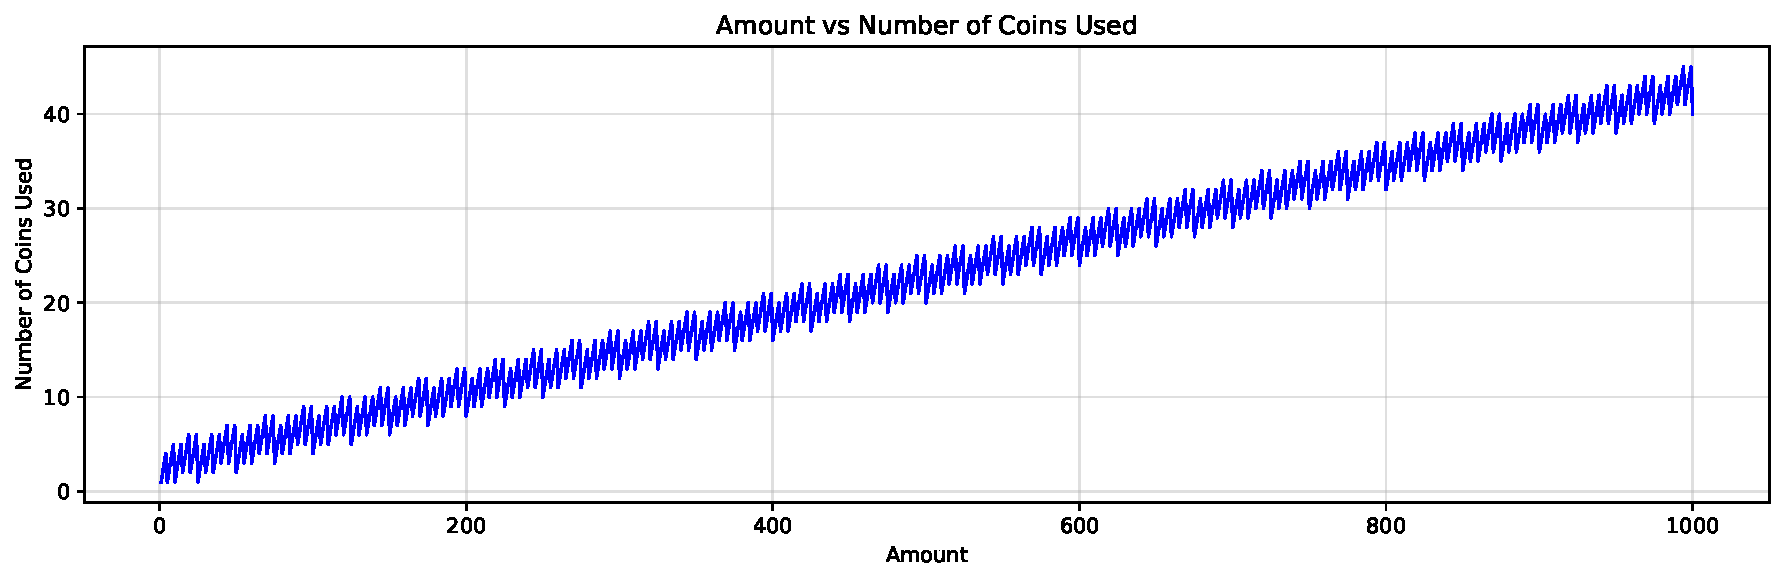
\includegraphics[width=\textwidth]{graphs/dp_coins_standard_plot.pdf}
  \caption{Number of coins used by the Dynamic Programming algorithm for the US coin system (denominations [1, 5, 10, 25]).}
  \label{fig:dp_coins_standard_plot}
\end{figure}

The above figure shows the relationship between the target amount and the number of coins selected by the Dynamic Programming (DP) algorithm for the standard US coin system. As expected, the number of coins increases approximately linearly with the target value, reflecting the additive construction of optimal solutions. Since the US coin system is canonical, the DP algorithm always produces the optimal (minimum-coin) result for every target, matching the Greedy approach in this case.

\begin{figure}[H]
  \centering
  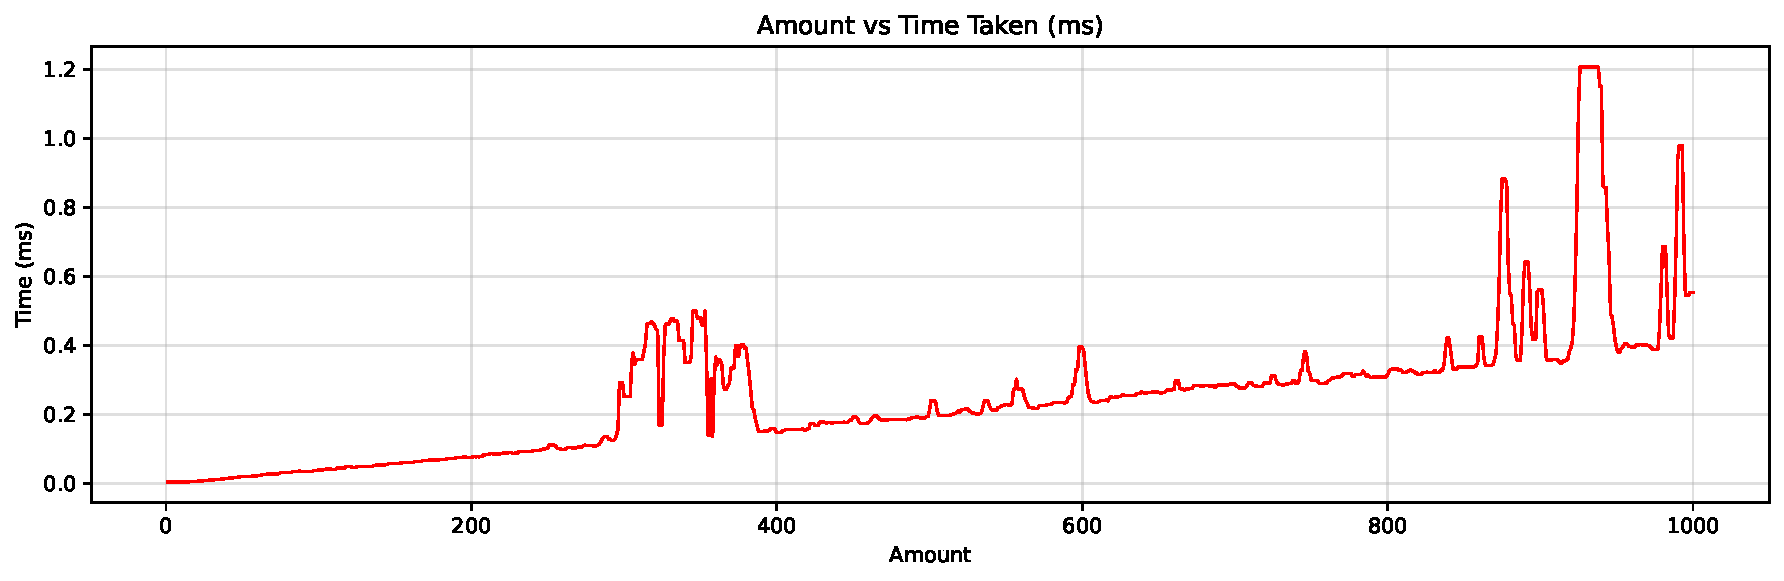
\includegraphics[width=\textwidth]{graphs/dp_time_standard_plot.pdf}
  \caption{Execution time of the Dynamic Programming algorithm for the US coin system.}
  \label{fig:dp_time_standard_plot}
\end{figure}

Figure~\ref{fig:dp_time_standard_plot} illustrates the execution time of the DP algorithm across the same target range. The runtime grows linearly with the target amount due to the iterative filling of the DP table, which maintains optimal coin counts for all intermediate values.

\begin{tcolorbox}[colback=gray!5!white, colframe=black, title=Note for the spikes in many runtime graph]
The small spikes observed in the execution time graphs are primarily due to memory management overhead, including memory allocation and cache behavior, as well as operating system scheduling and context switching. Even after applying smoothing techniques to reduce variability, these factors can introduce minor fluctuations in measured runtimes. Such spikes do not reflect the algorithm's intrinsic complexity, but rather the practical realities of executing the program in a general-purpose computing environment.
\end{tcolorbox}

Both the \textit{Amount vs. Time} and \textit{Amount vs. Minimum Number of Coins} graphs for the Dynamic Programming (DP) algorithm exhibited the expected linear growth with increasing target values. As the target amount increased, the number of coins required grew proportionally, reflecting the additive nature of the coin combination process. Similarly, the computation time scaled linearly with the target, as each additional value required updating the DP table. This behavior confirms the theoretical time and space efficiency of the DP algorithm for canonical coin systems.\\

The observed linear relationship between the target amount and both runtime and coin count remains consistent across other canonical coin systems as well. In the following examples—such as the Binary, Decimal, and Counting systems—the DP algorithm continues to yield optimal solutions, demonstrating its correctness and efficiency in all canonical settings. These cases collectively reinforce the theoretical guarantee that the DP method produces minimum-coin solutions regardless of the denomination structure.\\

\subsection{Canonical Examples: Dynamic Programming}
After observing the linear growth patterns in the standard US coin system, we extend the analysis to other \textbf{canonical coin systems} using the DP algorithm. Each case considers target values ranging from \textbf{1 to 1000}, and we analyze the performance of the DP algorithm in terms of \textbf{minimum coins used} and \textbf{execution time} for increasing amounts.\\

\begin{itemize}
  \item \textbf{Binary Coin System (1, 2, 4, 8, 16, 32)}\\
  This system represents denominations as powers of two. Each higher denomination is double the previous one, and the DP algorithm constructs the optimal solution iteratively for all target amounts. The following graphs show the number of coins used and execution time for targets 1--512.\\
  \begin{figure}[H]
    \centering
    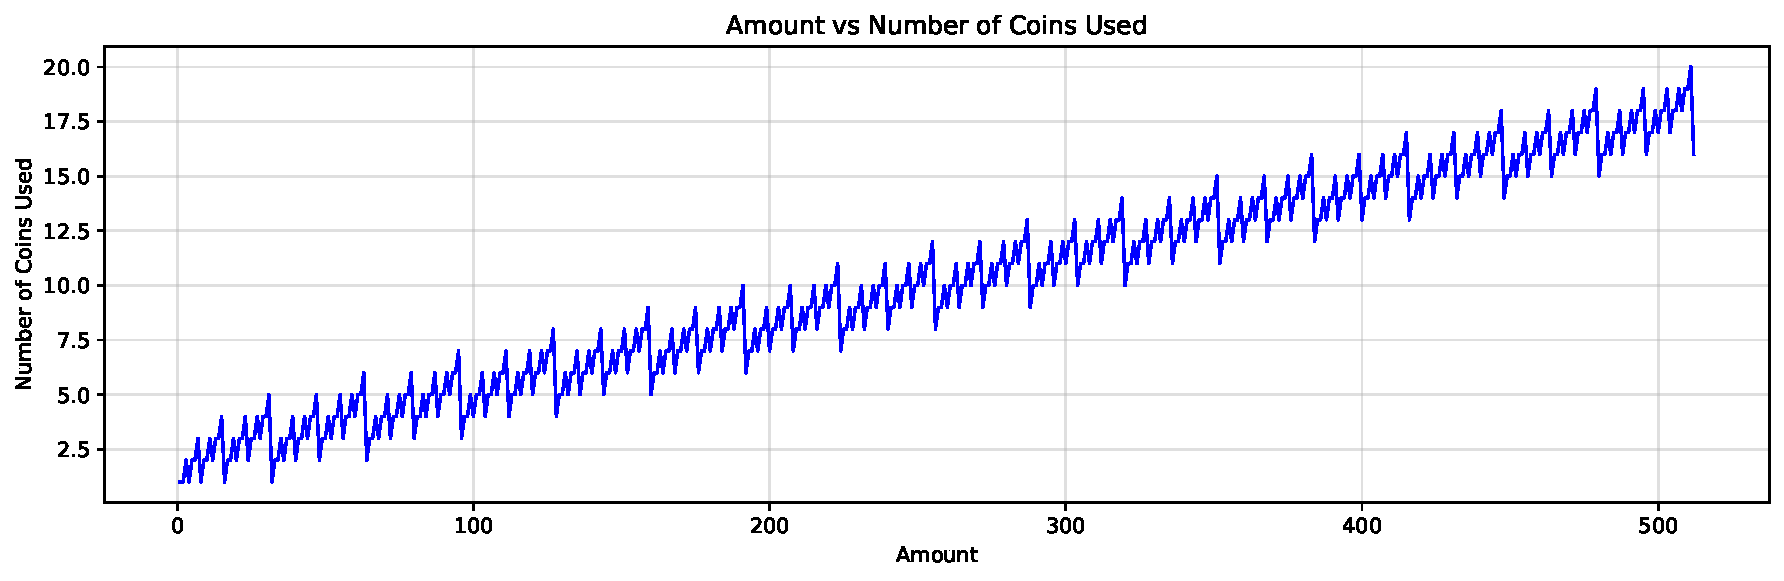
\includegraphics[width=\textwidth]{graphs/dp_coins_binary_plot.pdf}
    \caption{Dynamic Programming algorithm coin comparison for the Binary system (denominations [1, 2, 4, 8, 16, 32]) over targets 1--512.}
    \label{fig:dp_coins_binary_plot}
  \end{figure}

  \begin{figure}[H]
    \centering
    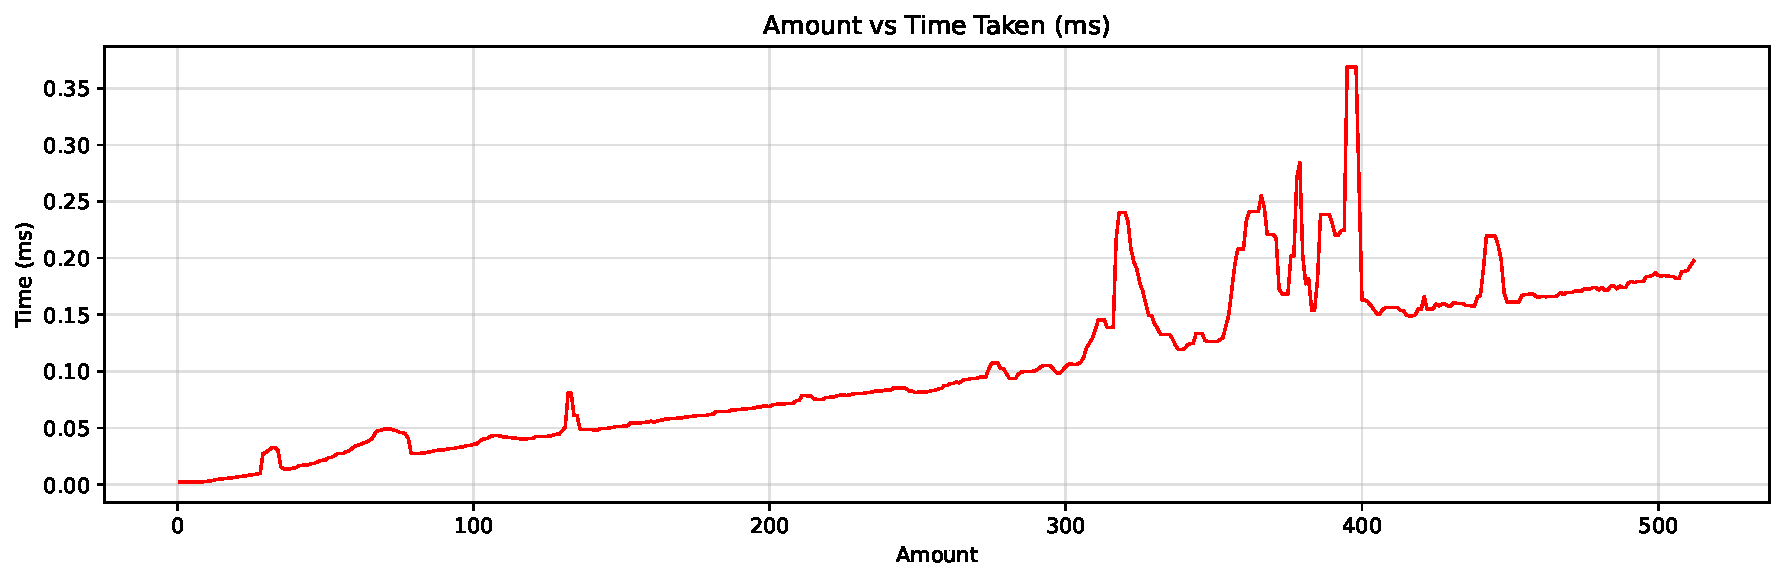
\includegraphics[width=\textwidth]{graphs/dp_time_binary_plot.pdf}
    \caption{Dynamic Programming algorithm time comparison for the Binary system (denominations [1, 2, 4, 8, 16, 32]) over targets 1--512.}
    \label{fig:dp_time_binary_plot}
  \end{figure}

  \item \textbf{Decimal Coin System (1, 10, 100)}\\
  A base-10 analogue of the binary case. Each denomination is a multiple of 10, ensuring optimality. Targets from 1 to 1000 show linear increase in the number of coins and a predictable computation time due to DP table updates.\\
  \begin{figure}[H]
    \centering
    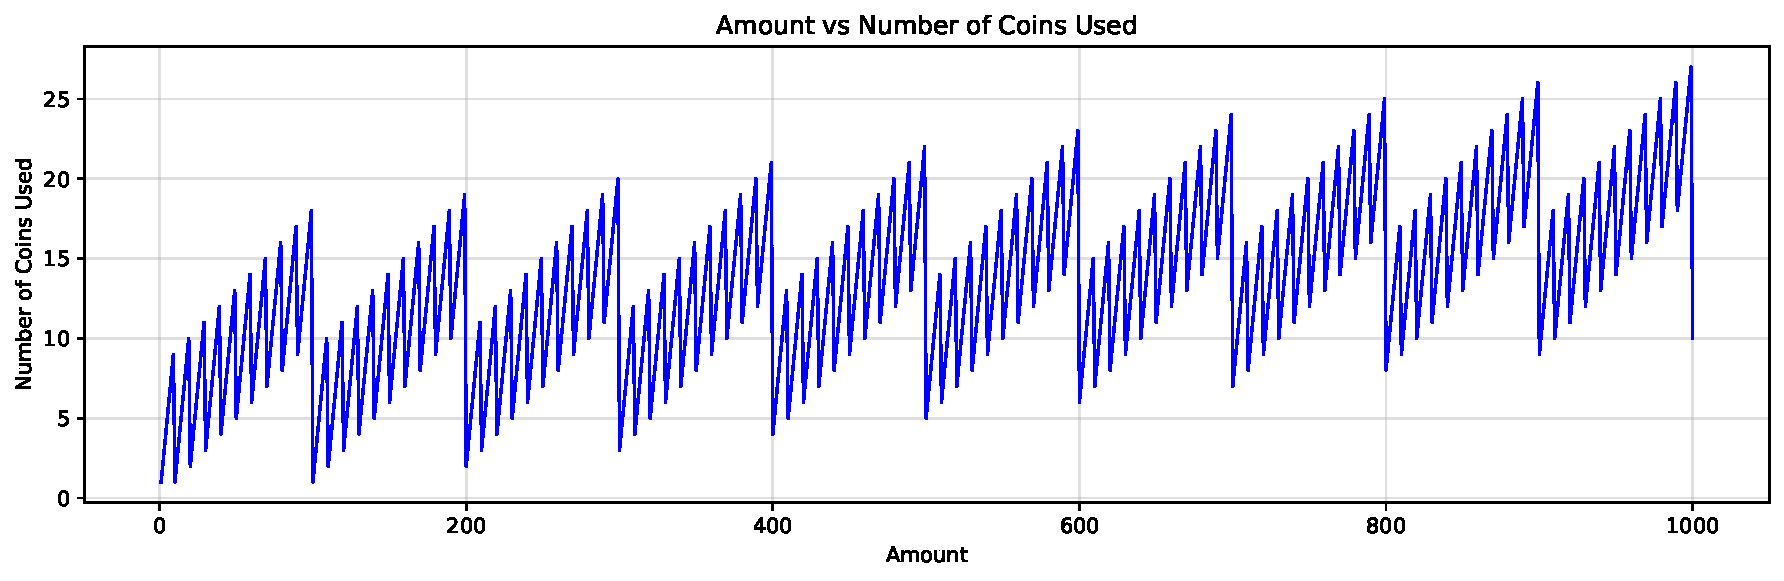
\includegraphics[width=\textwidth]{graphs/dp_coins_decimal_plot.pdf}
    \caption{Dynamic Programming algorithm coin comparison for the Decimal system (denominations [1, 10, 100]) over targets 1--1000.}
    \label{fig:dp_coins_decimal_plot}
  \end{figure}
  \begin{figure}[H]
    \centering
    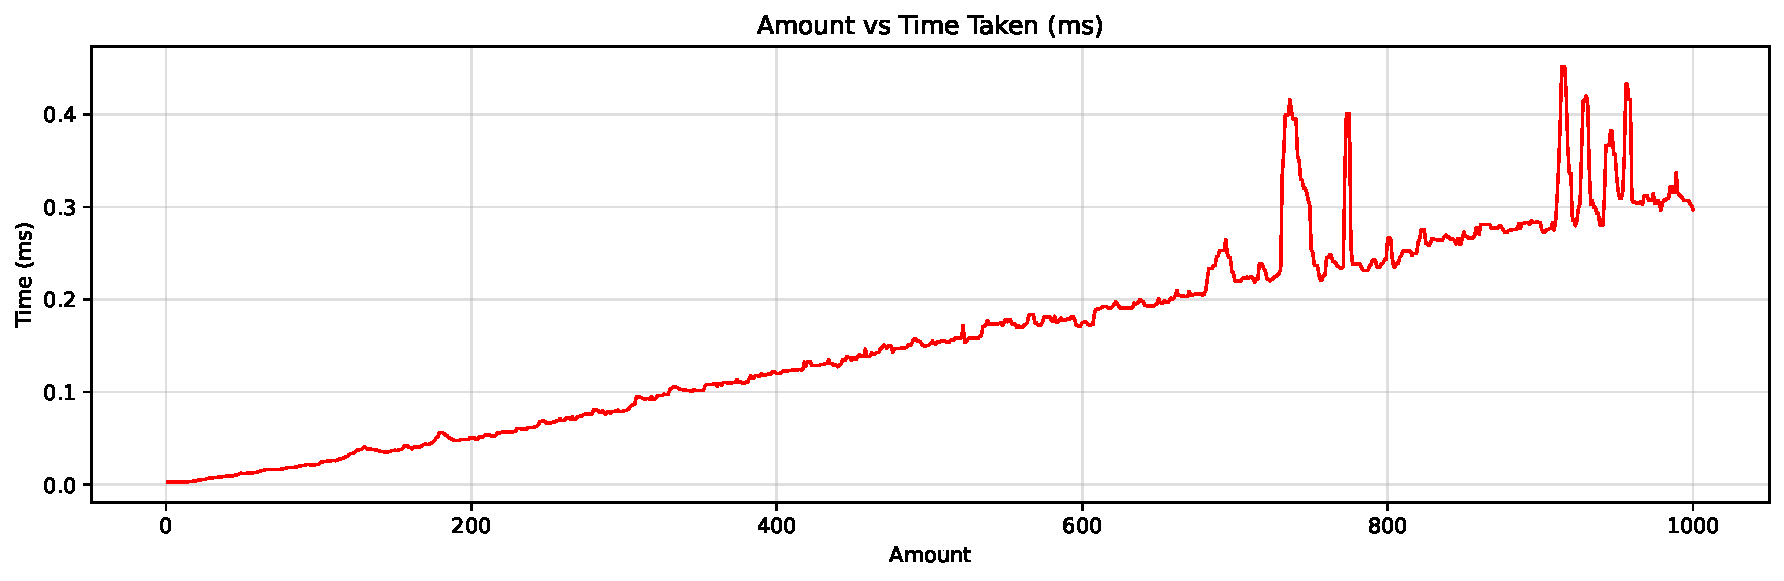
\includegraphics[width=\textwidth]{graphs/dp_time_decimal_plot.pdf}
    \caption{Dynamic Programming algorithm time comparison for the Decimal system (denominations [1, 10, 100]) over targets 1--1000.}
    \label{fig:dp_time_decimal_plot}
  \end{figure}

  \item \textbf{Counting Coin System (1, 2, 3, 4, 5, 6, 7)}\\
  This simple increasing system mimics counting numbers. The DP algorithm constructs optimal solutions for each target incrementally, guaranteeing minimum coins for all amounts. Both graphs display linear growth in coin count and a consistent increase in execution time across all target values.\\
  \begin{figure}[H]
    \centering
    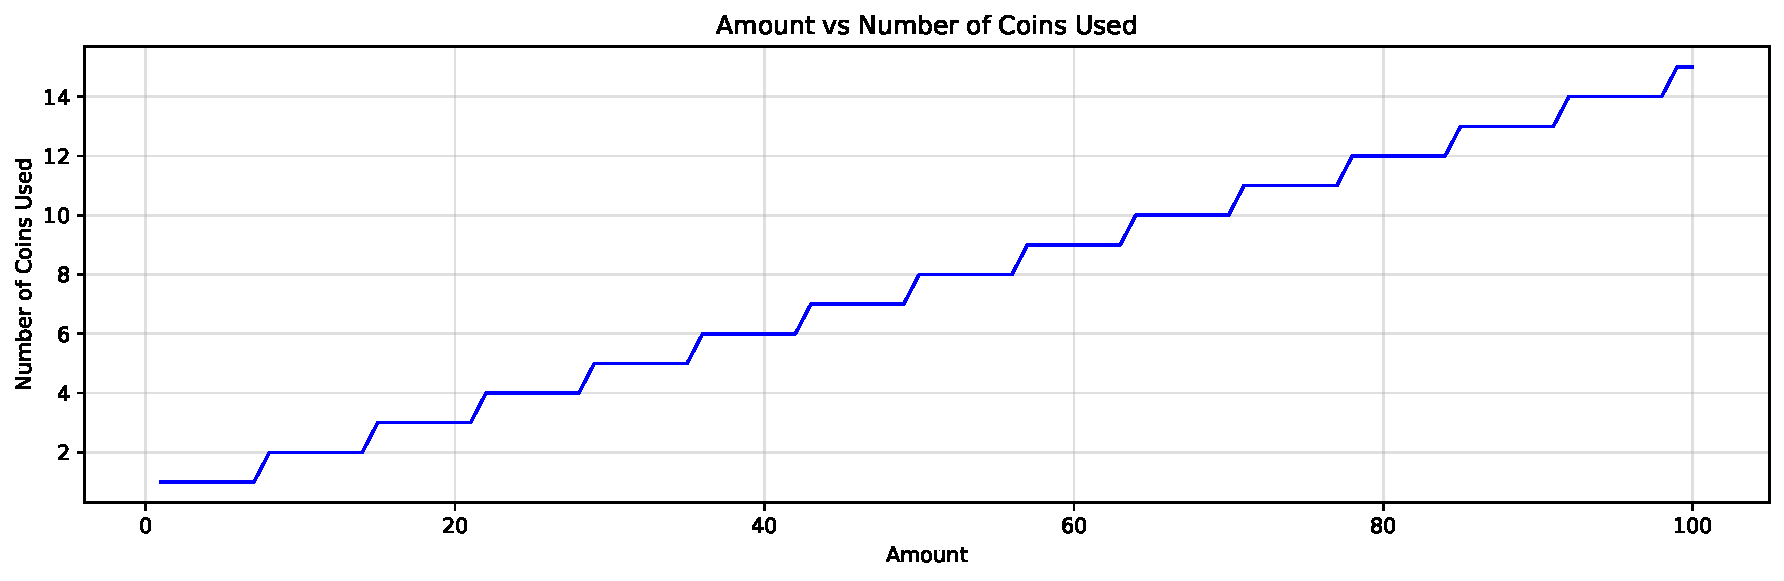
\includegraphics[width=\textwidth]{graphs/dp_coins_counting_plot.pdf}
    \caption{Dynamic Programming algorithm coin comparison for the Counting system (denominations [1, 2, 3, 4, 5, 6, 7]) over targets 1--100.}
    \label{fig:dp_coins_counting_plot}
  \end{figure}

  \begin{figure}[H]
    \centering
    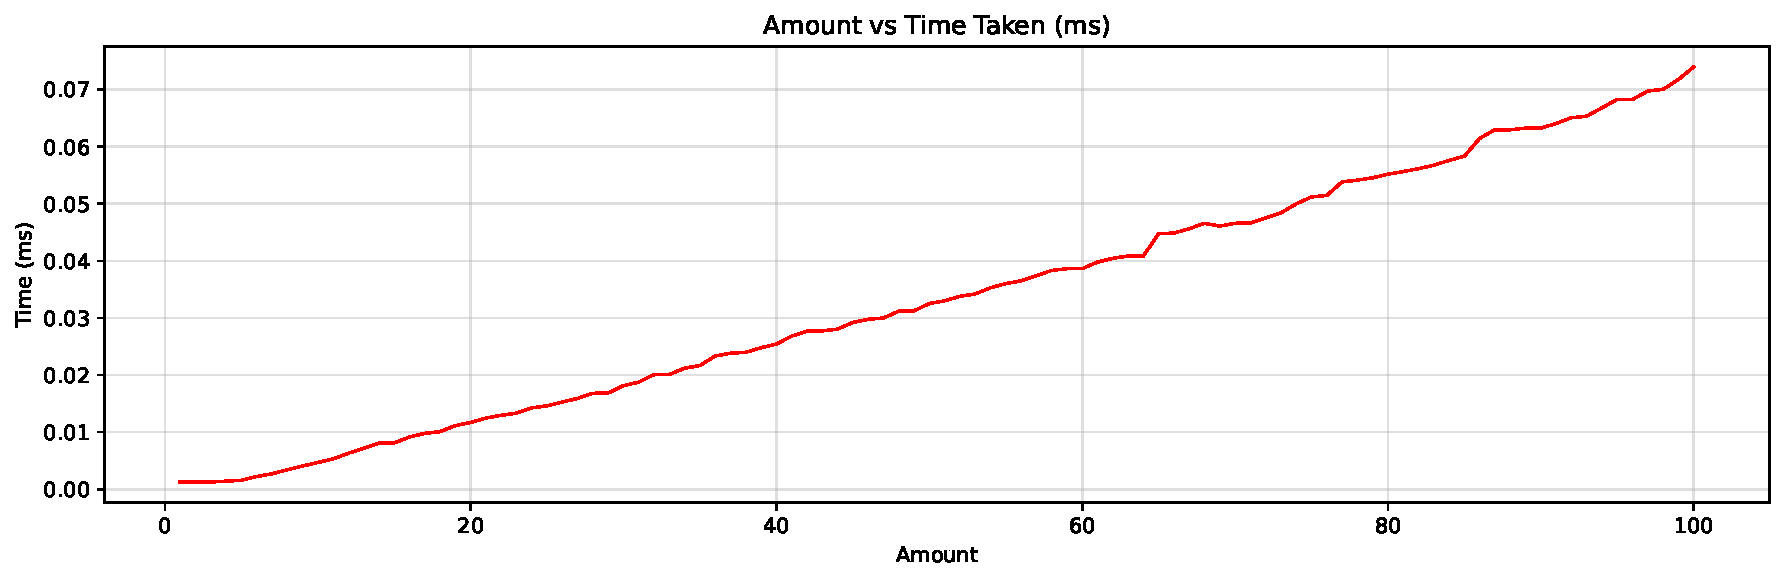
\includegraphics[width=\textwidth]{graphs/dp_time_counting_plot.pdf}
    \caption{Dynamic Programming algorithm time comparison for the Counting system (denominations [1, 2, 3, 4, 5, 6, 7]) over targets 1--100.}
    \label{fig:dp_time_counting_plot}
  \end{figure}
\end{itemize}

Both the \textit{Amount vs. Time} and \textit{Amount vs. Minimum Number of Coins} graphs for the Dynamic Programming (DP) algorithm in non-canonical coin systems illustrate optimal behavior across all targets. Unlike the Greedy approach, DP guarantees the minimum number of coins for every target amount, regardless of denomination structure. The computation time scales linearly with the target due to iterative table updates, and the coin count follows the true minimum solution.

\subsection{Non-Canonical Examples: Dynamic Programming}
We now analyze several \textbf{non-canonical coin systems} using the DP algorithm. Each system presents target ranges where the Greedy algorithm may fail, but DP consistently provides the correct minimum number of coins.

\begin{itemize}
    \item \textbf{Old Indian Coin System (1, 2, 5, 10, 20, 25, 50) paise}\\
    This historical coin system contains denominations that do not strictly satisfy canonical conditions. DP guarantees the minimum coins for all targets 1--500. For example, targets such as 40 or 75 are correctly solved by DP.\\
    \begin{figure}[H]
      \centering
      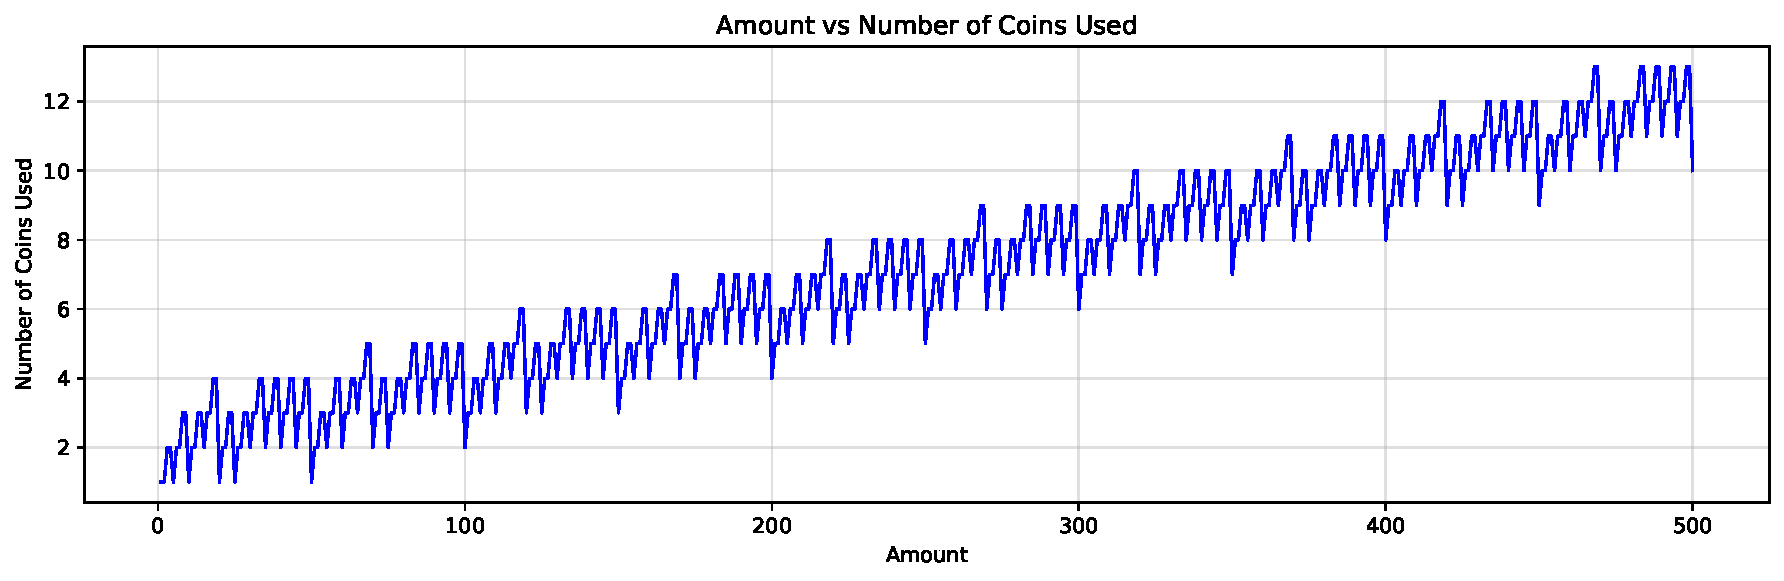
\includegraphics[width=\textwidth]{graphs/dp_coins_indiancoinsystum_plot.pdf}
      \caption{Number of coins used by the Dynamic Programming algorithm for the Old Indian Coin System over targets 1--500.}
      \label{fig:dp_coins_indiancoinsystum_plot}
    \end{figure}
    \begin{figure}[H]
      \centering
      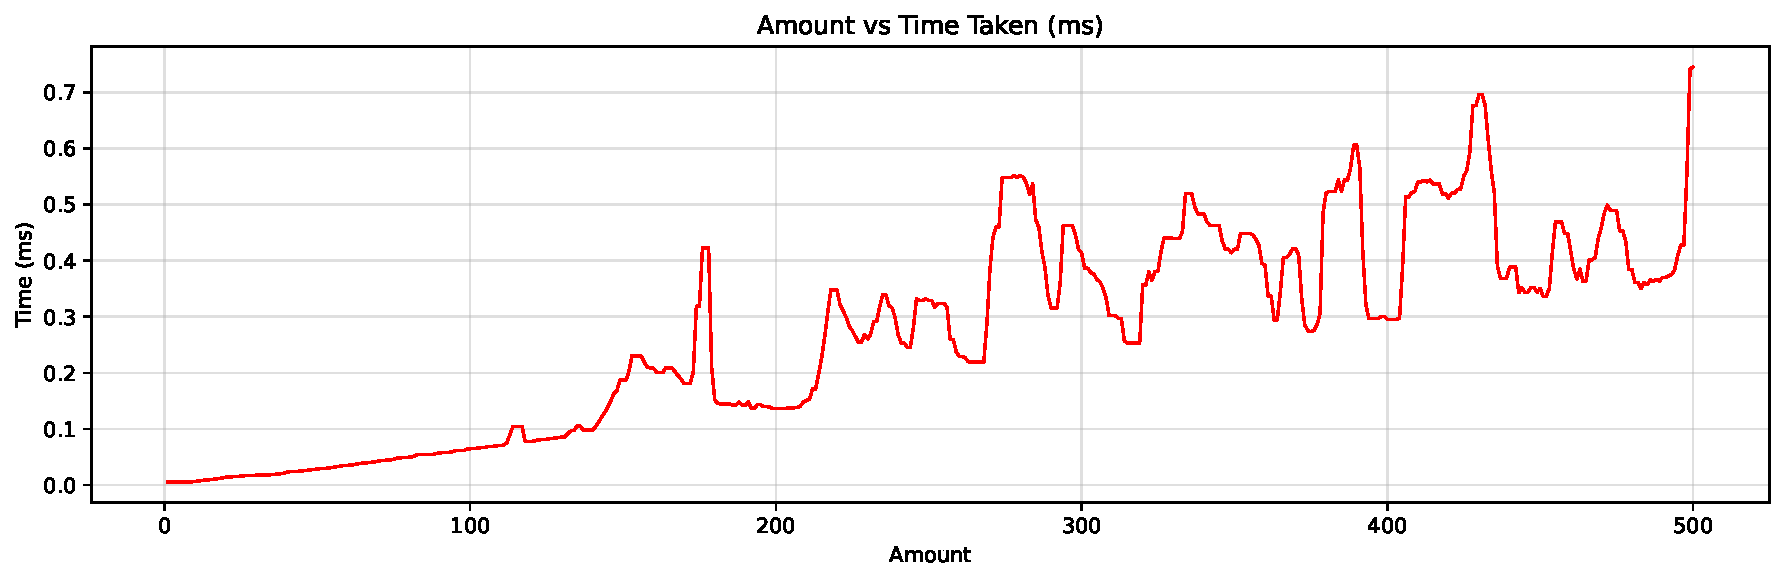
\includegraphics[width=\textwidth]{graphs/dp_time_indiancoinsystum_plot.pdf}
      \caption{Execution time of the Dynamic Programming algorithm for the Old Indian Coin System.}
      \label{fig:dp_time_indiancoinsystum_plot}
    \end{figure}
\newpage
    \item \textbf{Square Coin System (1, 4, 9, 16, 25, 36, 49)}\\
    Denominations are perfect squares, making this system non-canonical. DP finds the minimum coins for all targets 1--441, including targets like 18 or 27 where Greedy fails.\\
    \begin{figure}[H]
      \centering
      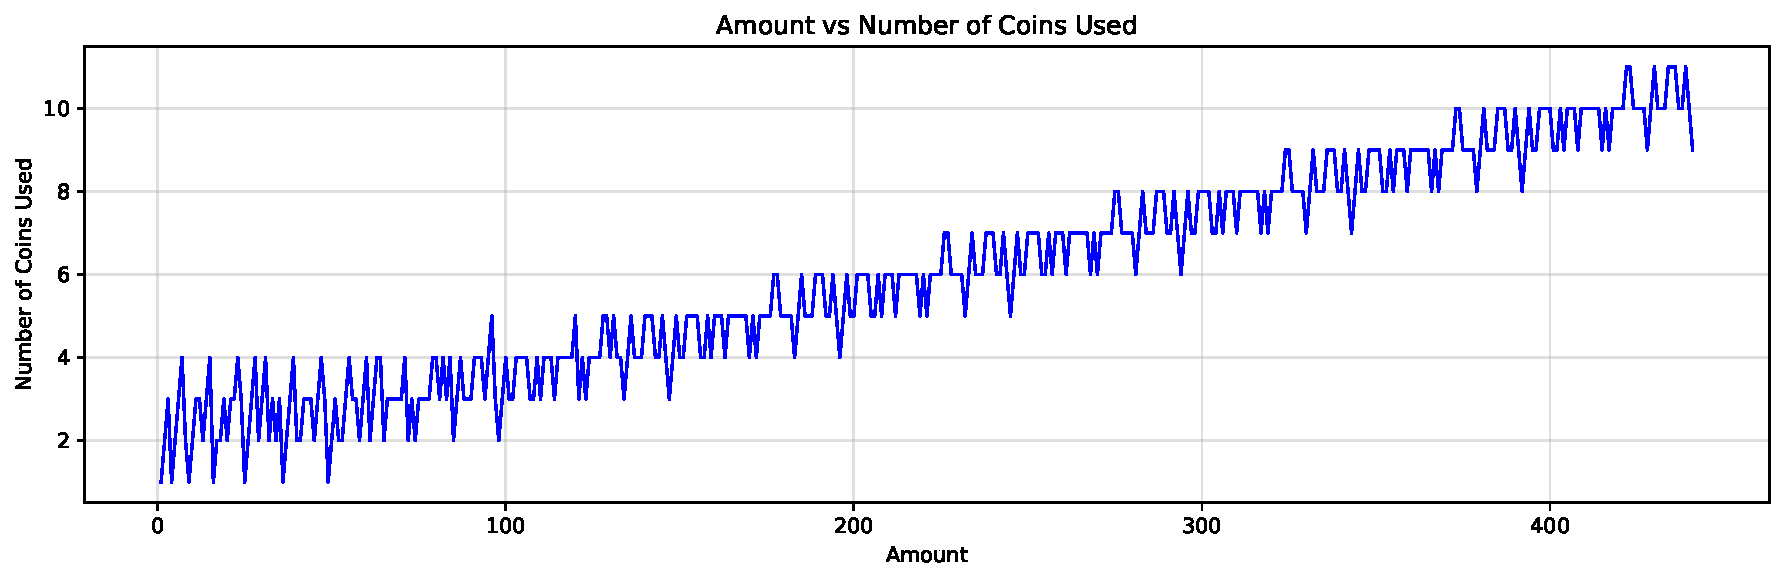
\includegraphics[width=\textwidth]{graphs/dp_coins_square_plot.pdf}
      \caption{Number of coins used by the Dynamic Programming algorithm for the Square coin system over targets 1--441.}
      \label{fig:dp_coins_square_plot}
    \end{figure}
    \begin{figure}[H]
      \centering
      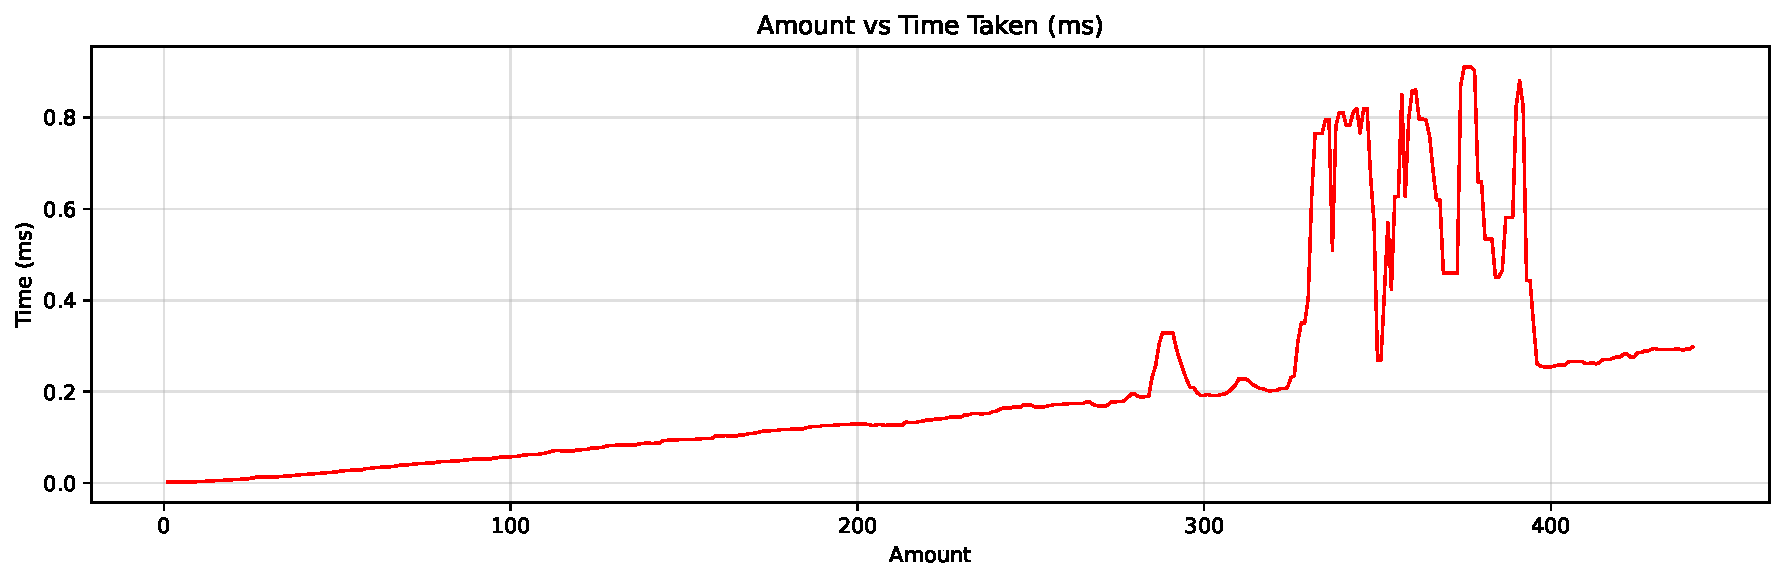
\includegraphics[width=\textwidth]{graphs/dp_time_square_plot.pdf}
      \caption{Execution time of the Dynamic Programming algorithm for the Square coin system.}
      \label{fig:dp_time_square_plot}
    \end{figure}

    \item \textbf{Twin Prime Coin System (1, 41, 43, 101, 103)}\\
    Denominations are based on twin primes. DP computes the minimum coins correctly for all targets 1--431, including cases like 83 where Greedy fails.\\
    \begin{figure}[H]
      \centering
      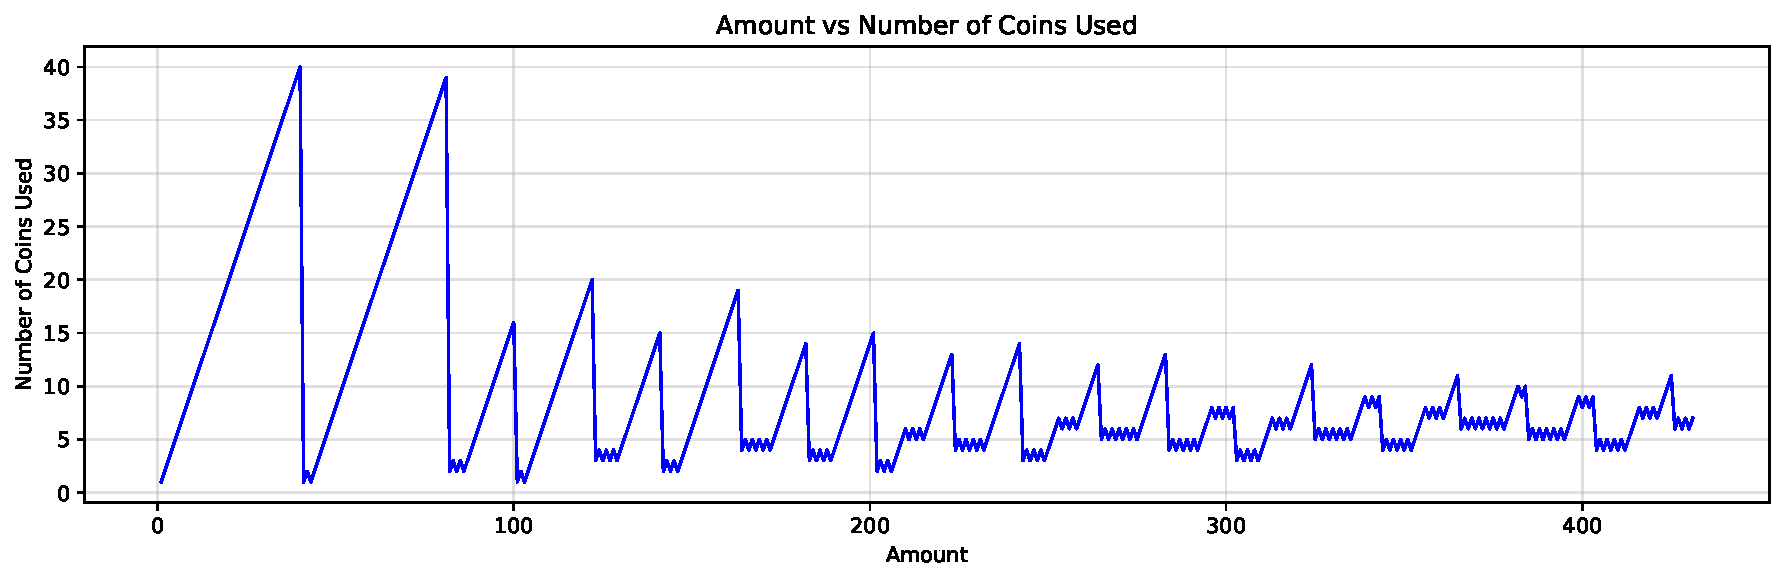
\includegraphics[width=\textwidth]{graphs/dp_coins_twin_prime_plot.pdf}
      \caption{Number of coins used by the Dynamic Programming algorithm for the Twin Prime coin system over targets 1--431.}
      \label{fig:dp_coins_twin_prime_plot}
    \end{figure}
    \begin{figure}[H]
      \centering
      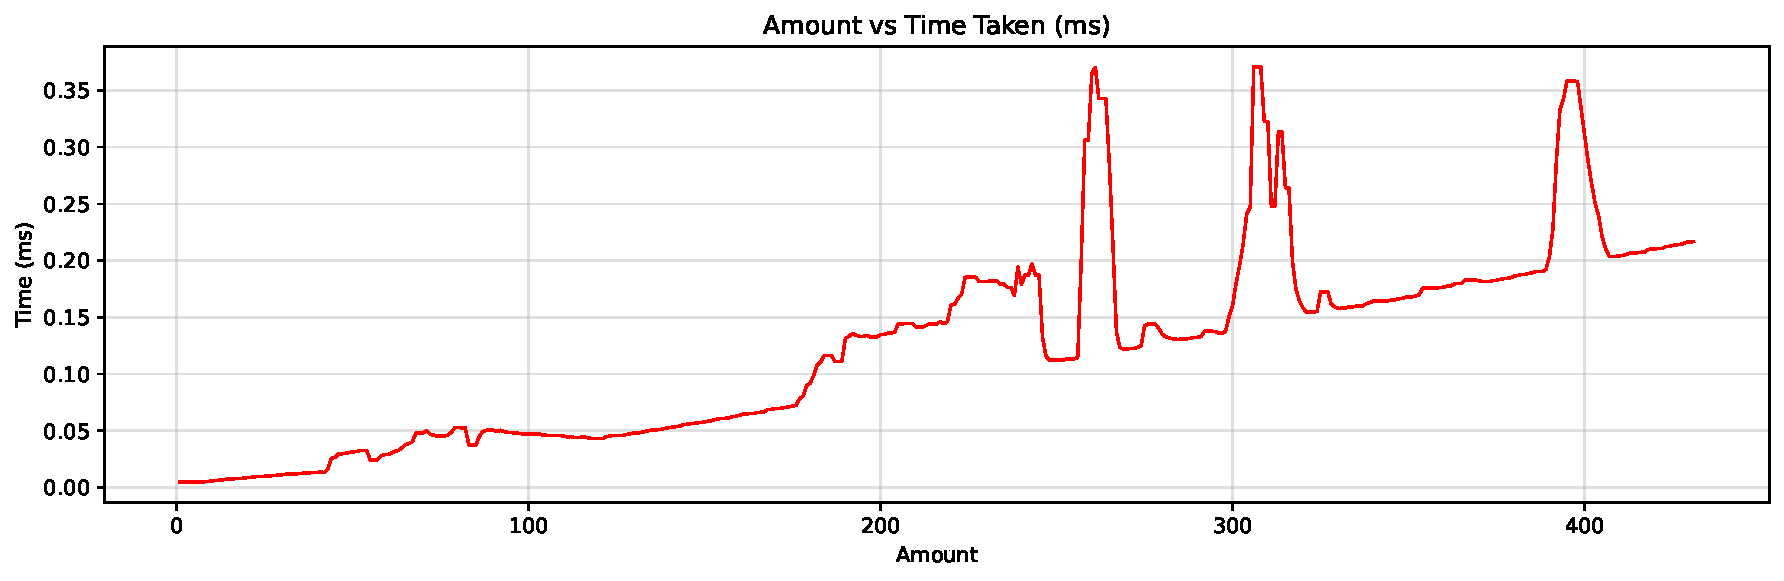
\includegraphics[width=\textwidth]{graphs/dp_time_twin_prime_plot.pdf}
      \caption{Execution time of the Dynamic Programming algorithm for the Twin Prime coin system.}
      \label{fig:dp_time_twin_prime_plot}
    \end{figure}

\item \textbf{Meme Number Coin System (1, 6, 7, 69, 420)}\\
Denominations are inspired by well-known internet meme numbers. The system is highly non-canonical, causing the Greedy algorithm to fail for many targets. For instance, for target 12, Greedy chooses one 7-coin and five 1-coins (6 coins total), whereas the optimal solution uses two 6-coins (2 coins total).\\
Dynamic Programming (DP) correctly computes the minimum number of coins for all targets 1--666, ensuring optimality even in irregular systems like this one.\\

\begin{figure}[H]
  \centering
  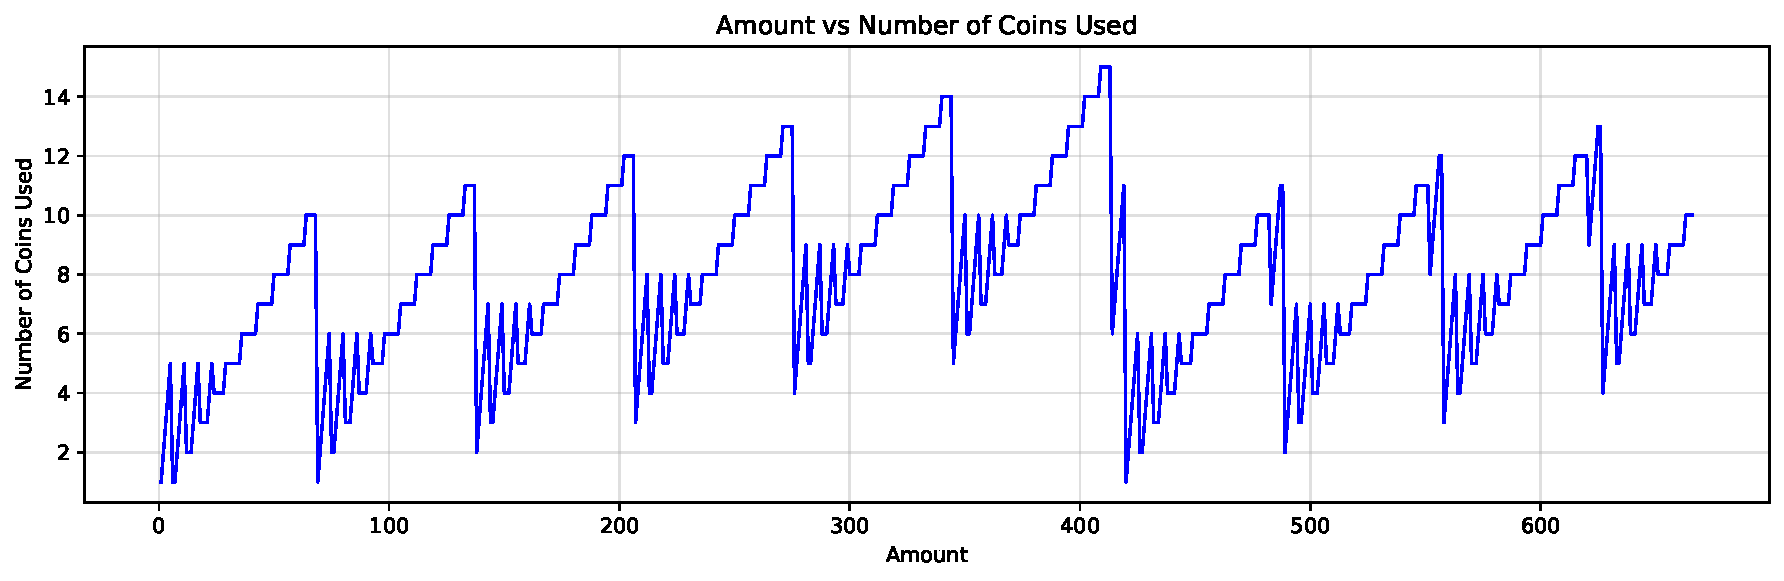
\includegraphics[width=\textwidth]{graphs/dp_coins_meme_plot.pdf}
  \caption{Number of coins used by the Dynamic Programming algorithm for the Meme Number coin system over targets 1--666.}
  \label{fig:dp_coins_meme_number_plot}
\end{figure}

\begin{figure}[H]
  \centering
  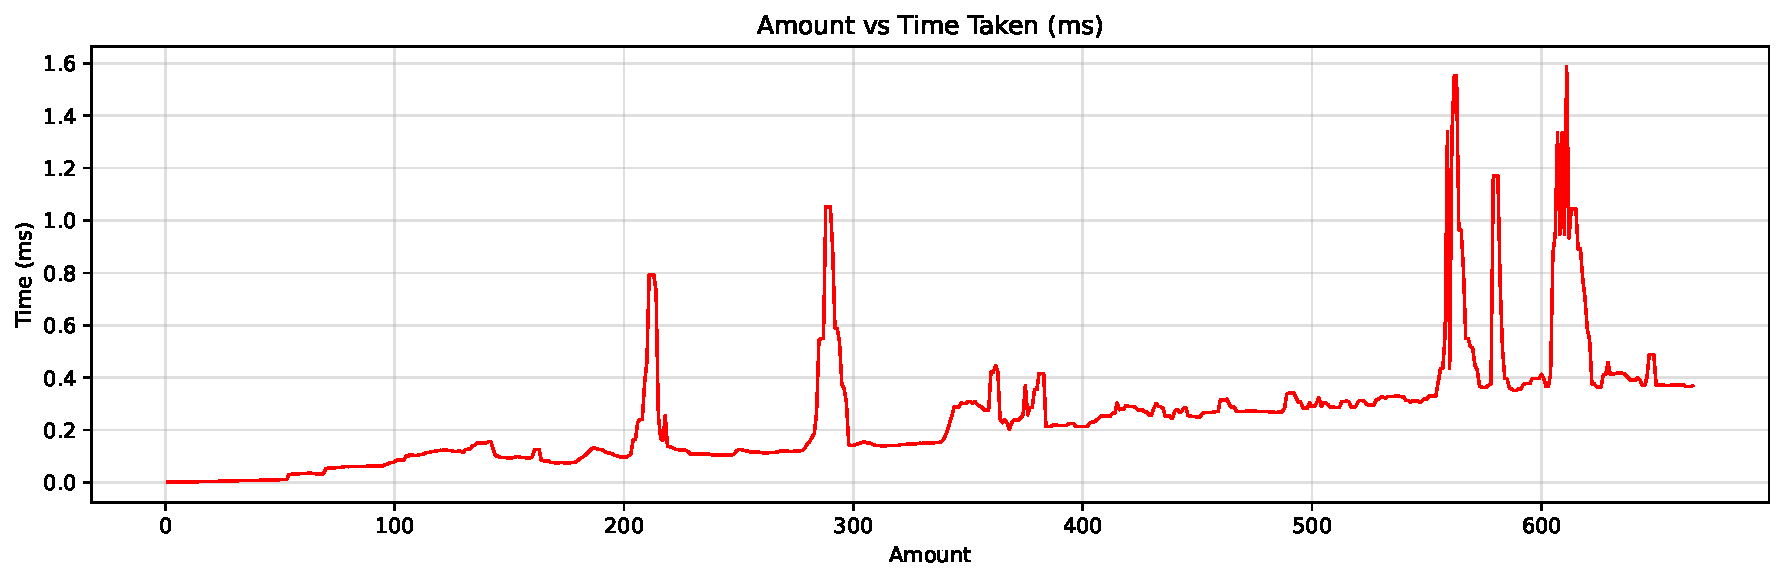
\includegraphics[width=\textwidth]{graphs/dp_time_meme_plot.pdf}
  \caption{Execution time of the Dynamic Programming algorithm for the Meme Number coin system.}
  \label{fig:dp_time_meme_number_plot}
\end{figure}
\end{itemize}

\section{Conclusion}
\label{sec:dp_conclusion}

In this chapter, we explored the Dynamic Programming (DP) approach to the Coin Change problem in detail. We began by motivating the use of DP (Section~2.1) and provided the corresponding pseudocode (Section~2.2), followed by a formal proof of correctness (Section~2.3). The analysis of time and space complexity (Section~2.4) showed that the algorithm efficiently computes minimum coin counts for all targets up to a specified range, with complexity proportional to the product of the target amount and the number of denominations. Section~2.5 presented a Python implementation, and Section~2.6 demonstrated experimental results across both canonical and non-canonical coin systems.

The results confirm that the DP algorithm consistently produces the minimum number of coins for every target, independent of the coin system structure. Unlike the Greedy algorithm, DP guarantees optimality even in non-canonical systems where Greedy fails. Runtime scales predictably with the target amount, and the algorithm remains practical for reasonably large target ranges. Overall, this chapter illustrates the robustness and reliability of Dynamic Programming for solving the Coin Change problem, establishing it as a general-purpose method capable of handling both canonical and non-canonical coin systems.


%=========================================================================================================================================================================================================================================


\chapter{Comparison of Greedy and Dynamic Programming Approaches \centering}
\section{Introduction}
\label{sec:comparison_intro}

This chapter provides a detailed comparison between the Greedy and Dynamic Programming (DP) algorithms for the Coin Change problem. While both algorithms aim to minimize the number of coins required for a given target amount, their correctness and efficiency vary depending on the structure of the coin denominations. 

Greedy is simple, fast, and works optimally for canonical coin systems, where each larger denomination is a multiple or suitable combination of smaller ones. However, for non-canonical systems, Greedy can fail to produce the minimum number of coins. Dynamic Programming, on the other hand, guarantees the optimal solution for all target amounts, regardless of the coin system, by constructing solutions iteratively and storing intermediate results.

The objective of this chapter is to analyze both algorithms across multiple coin systems, compare their performance in terms of coin count and execution time, and highlight scenarios where Greedy fails and DP provides the correct solution. Through experimental datasets and graphical representations, the chapter demonstrates the trade-offs between simplicity, efficiency, and correctness in algorithm selection.

\section{Experimental Setup}
\label{sec:comparison_experimental_setup}

In order to systematically compare the Greedy and Dynamic Programming (DP) algorithms, we designed a set of experiments covering both canonical and non-canonical coin systems. The setup ensures consistent and repeatable measurement of algorithm performance across varying target amounts.

\subsection{Coin Systems and Target Ranges}
The experiments were conducted on the following coin systems:

\begin{itemize}
    \item \textbf{Canonical Systems:}
    \begin{itemize}
        \item \textbf{Standard US Coin System:} Denominations [1, 5, 10, 25], target range 1--1000.
        \item \textbf{Binary System:} Denominations [1, 2, 4, 8, 16, 32], target range 1--512.
        \item \textbf{Decimal System:} Denominations [1, 10, 100], target range 1--1000.
        \item \textbf{Counting System:} Denominations [1, 2, 3, 4, 5, 6, 7], target range 1--100.
    \end{itemize}
    
    \item \textbf{Non-Canonical Systems:}
    \begin{itemize}
        \item \textbf{Old Indian Coin System:} Denominations [1, 2, 5, 10, 20, 25, 50], target range 1--500.
        \item \textbf{Square System:} Denominations [1, 4, 9, 16, 25, 36, 49], target range 1--441.
        \item \textbf{Twin Prime System:} Denominations [1, 41, 43, 101, 103], target range 1--431.
    \end{itemize}
\end{itemize}

\subsection{Algorithm Implementation}
\begin{itemize}
    \item \textbf{Greedy Algorithm:} Implements a simple iterative approach selecting the largest possible coin at each step. Guarantees optimality for canonical systems.
    \item \textbf{Dynamic Programming Algorithm:} Builds a DP table iteratively, storing the minimum coins required for all amounts up to the target. Guarantees optimality for all systems, including non-canonical ones.
\end{itemize}

\subsection{Performance Metrics}
The following metrics were measured for each algorithm and coin system:
\begin{itemize}
    \item \textbf{Number of Coins Used:} Minimum number of coins required to make each target amount.
    \item \textbf{Execution Time:} Time taken to compute the coin combination for each target amount. Measured using high-precision timers and averaged over multiple runs to reduce noise.
\end{itemize}

\subsection{Data Collection and Graph Generation}
For each coin system and algorithm:
\begin{itemize}
    \item Results were saved in CSV files containing \textit{Amount}, \textit{No. of Coins Used}, and \textit{Execution Time}.
    \item Graphs were generated for each system, showing:
        \begin{itemize}
            \item Target Amount vs. Minimum Number of Coins.
            \item Target Amount vs. Execution Time.
        \end{itemize}
    \item For canonical systems, Greedy and DP graphs were compared to demonstrate equivalence.
    \item For non-canonical systems, Greedy failures were highlighted alongside DP results to show guaranteed optimality.
\end{itemize}

\section{Comparison on Canonical Systems}
\label{sec:comparison_canonical}

This section analyzes the performance of the Greedy and Dynamic Programming (DP) algorithms on canonical coin systems, where the Greedy approach is guaranteed to produce optimal results. The objective is to demonstrate that both algorithms yield the same minimum number of coins, while also comparing execution times.

\subsection{Standard US Coin System}
The Standard US coin system consists of denominations [1, 5, 10, 25], with target amounts ranging from 1 to 1000. As expected, the Greedy algorithm produces optimal coin combinations identical to those generated by DP.

\begin{figure}[H]
  \centering
  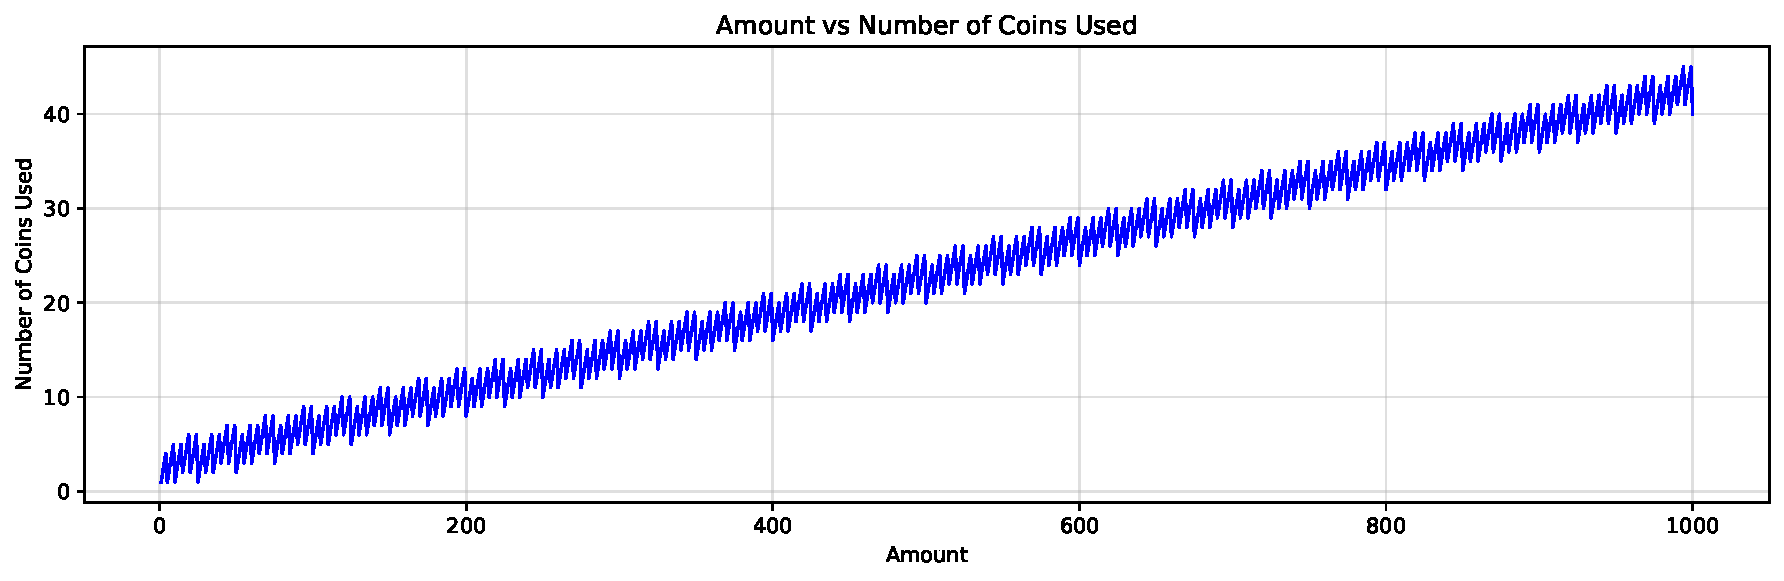
\includegraphics[width=\textwidth]{graphs/greedy_coins_standard_plot.pdf}
  \caption{Number of coins used by the Greedy algorithm for the US coin system (denominations [1, 5, 10, 25]).}
  \label{fig:greedy_coins_standard}
\end{figure}

\begin{figure}[H]
  \centering
  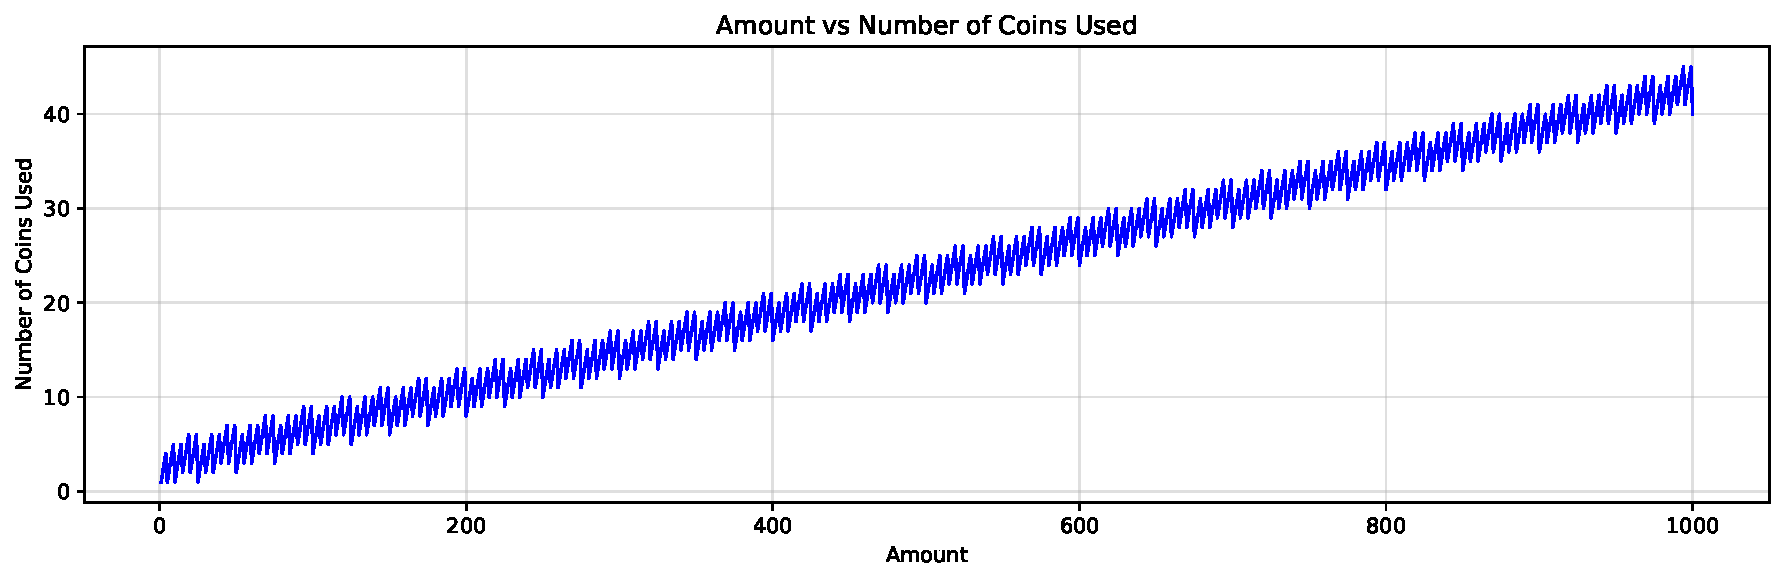
\includegraphics[width=\textwidth]{graphs/dp_coins_standard_plot.pdf}
  \caption{Number of coins used by the Dynamic Programming algorithm for the US coin system.}
  \label{fig:dp_coins_standard}
\end{figure}

\begin{figure}[H]
  \centering
  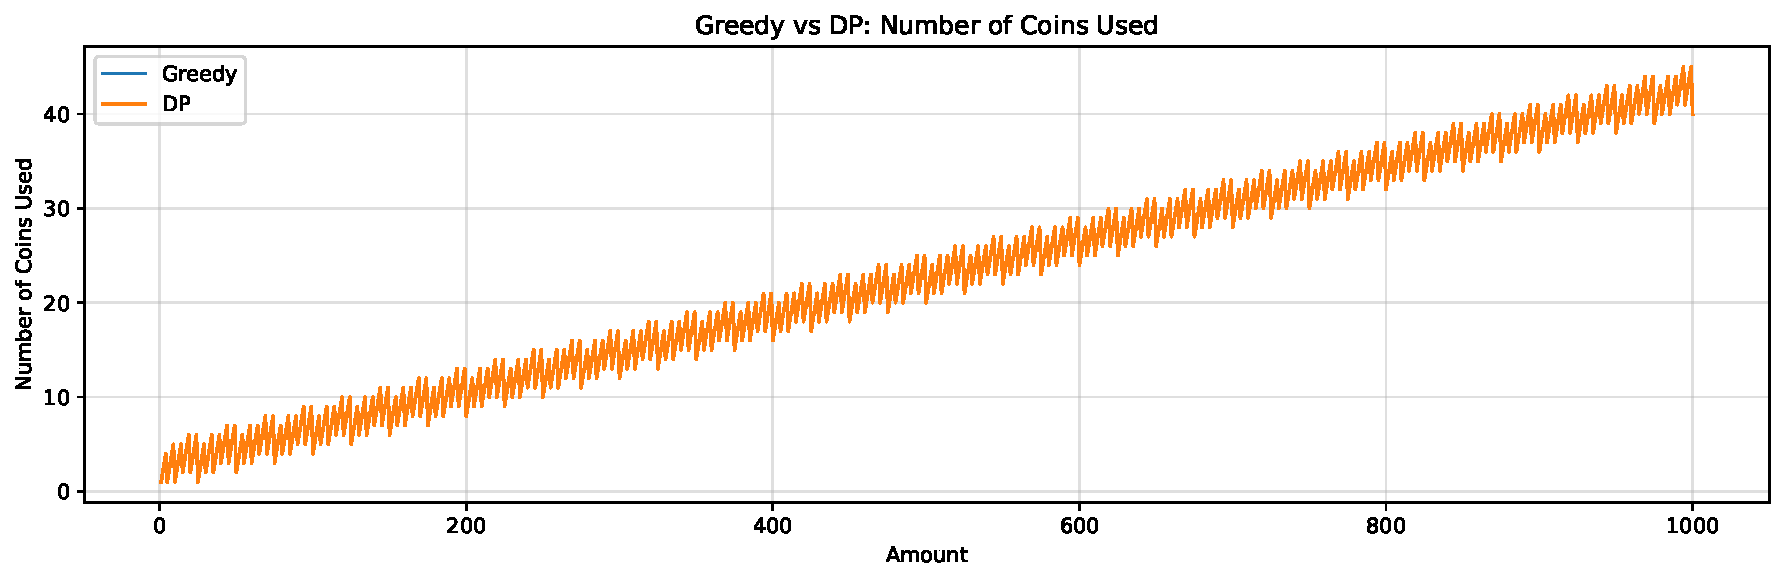
\includegraphics[width=\textwidth]{graphs/compare_coins_standard_plot.pdf}
  \caption{Comparison of minimum coins between Greedy and DP for the US coin system. Both algorithms produce identical results.}
  \label{fig:compare_coins_standard}
\end{figure}

Now we'll look ta the time graphs for Standard US coin system. \\
Execution time comparisons show that Greedy is consistently faster due to its iterative selection process, while DP requires table construction.

\begin{figure}[H]
  \centering
  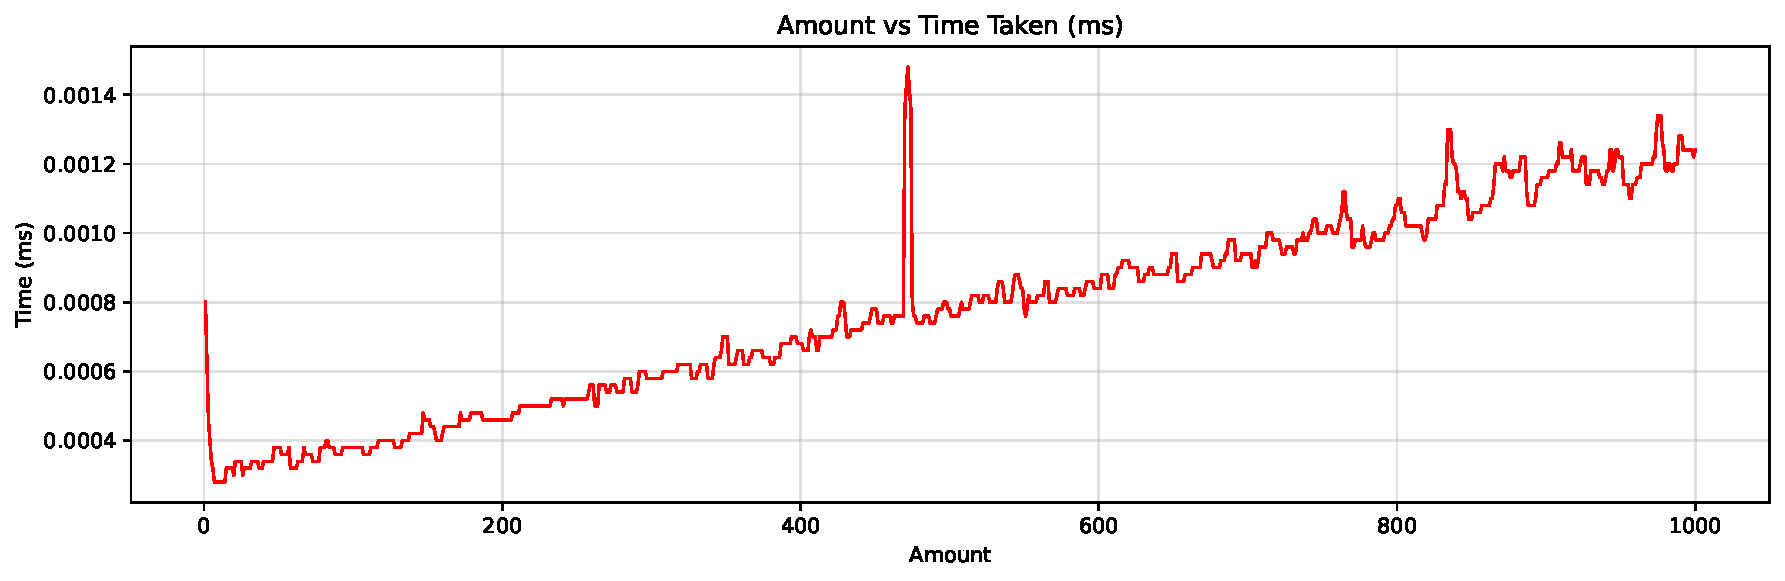
\includegraphics[width=\textwidth]{graphs/greedy_time_standard_plot.pdf}
  \caption{Execution time of the Greedy algorithm for the US coin system.}
  \label{fig:greedy_time_standard}
\end{figure}

\begin{figure}[H]
  \centering
  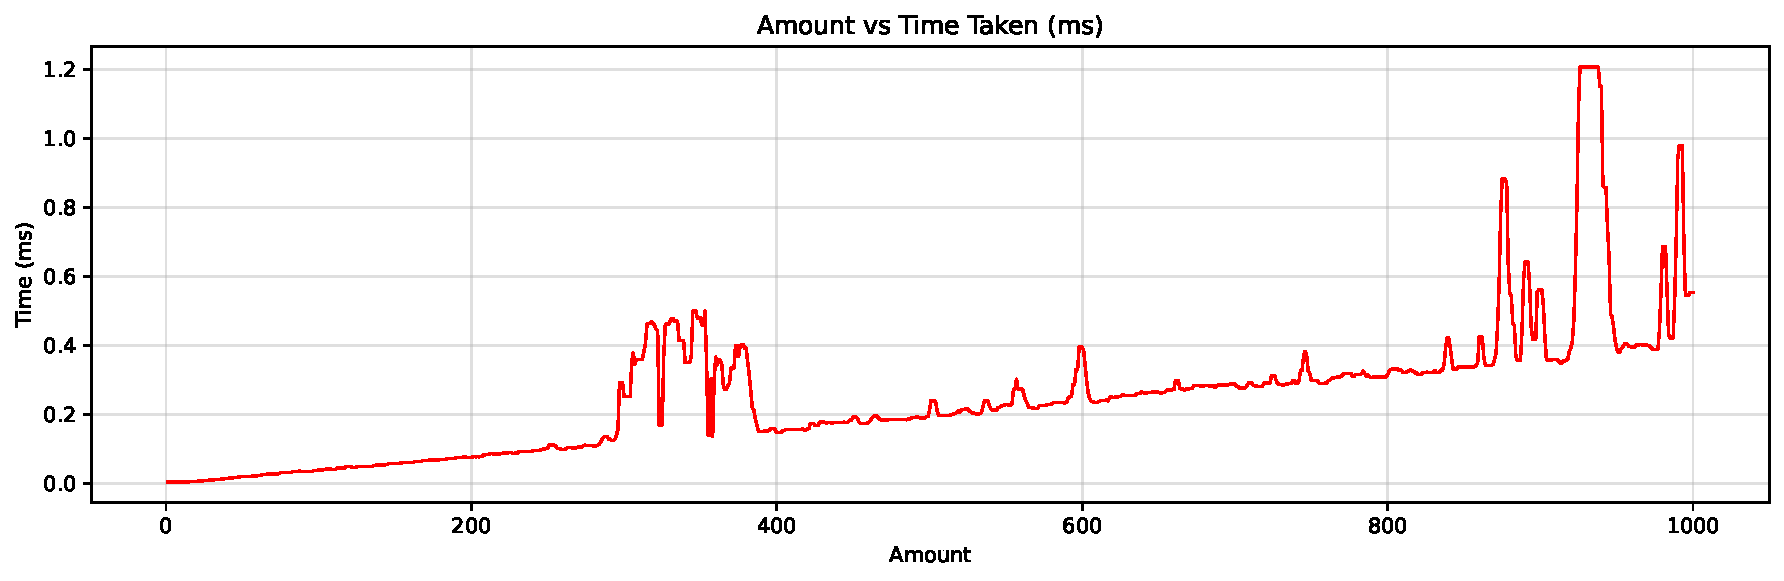
\includegraphics[width=\textwidth]{graphs/dp_time_standard_plot.pdf}
  \caption{Execution time of the Dynamic Programming algorithm for the US coin system.}
  \label{fig:dp_time_standard}
\end{figure}

\begin{figure}[H]
  \centering
  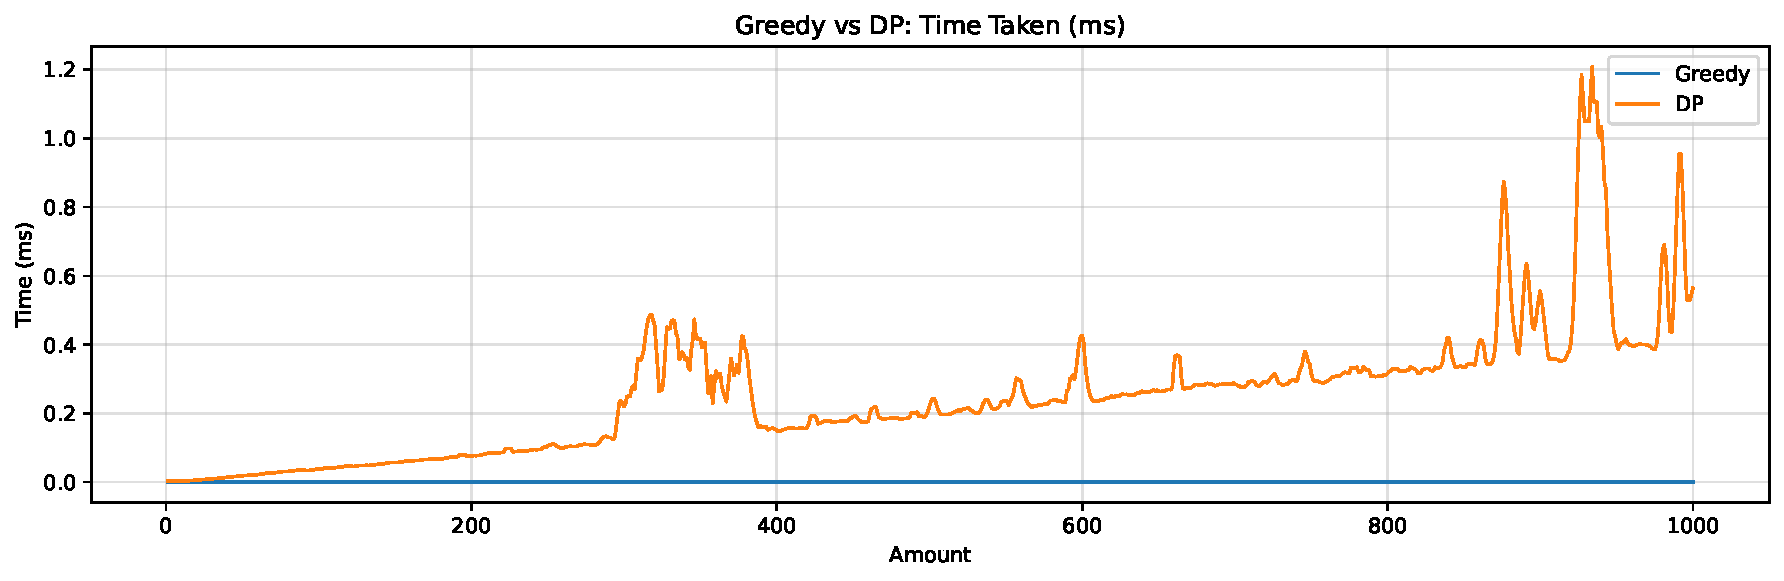
\includegraphics[width=\textwidth]{graphs/compare_time_standard_plot.pdf}
  \caption{Comparison of the execution times of the Greedy and Dynamic Programming algorithms for the US coin system.}
  \label{fig:compare_time_standard_plot}
\end{figure}

\begin{tcolorbox}[colback=gray!5!white, colframe=black, title=Execution Time Note]
The execution time comparison between Greedy and Dynamic Programming (DP) for canonical coin systems is consistent across all targets. While both algorithms produce the same minimum number of coins, the Greedy algorithm is significantly faster than DP due to its simple iterative selection process. Consequently, we do not include the runtime graphs here. 

For those interested in viewing the detailed time comparison graphs for all canonical systems, please refer to the project's GitHub repository: \url{}.
\end{tcolorbox}


\subsection{Binary Coin System}
Denominations are powers of two: [1, 2, 4, 8, 16, 32], target range 1--512. Greedy and DP produce identical minimum coin counts. The stepwise increase in coins is due to doubling denominations.

\begin{figure}[H]
  \centering
  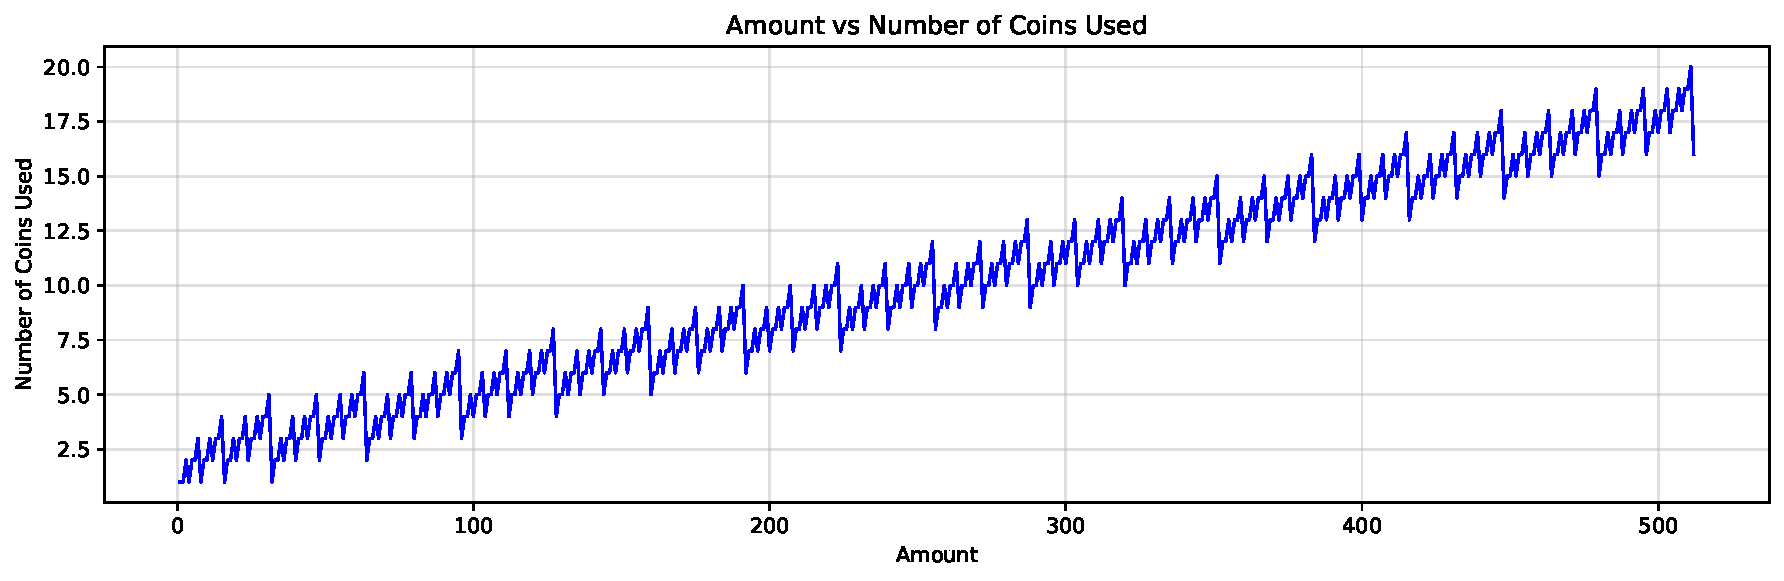
\includegraphics[width=\textwidth]{graphs/greedy_coins_binary_plot.pdf}
  \caption{Number of coins used by the Greedy algorithm for the Binary coin system.}
  \label{fig:greedy_coins_binary}
\end{figure}

\begin{figure}[H]
  \centering
  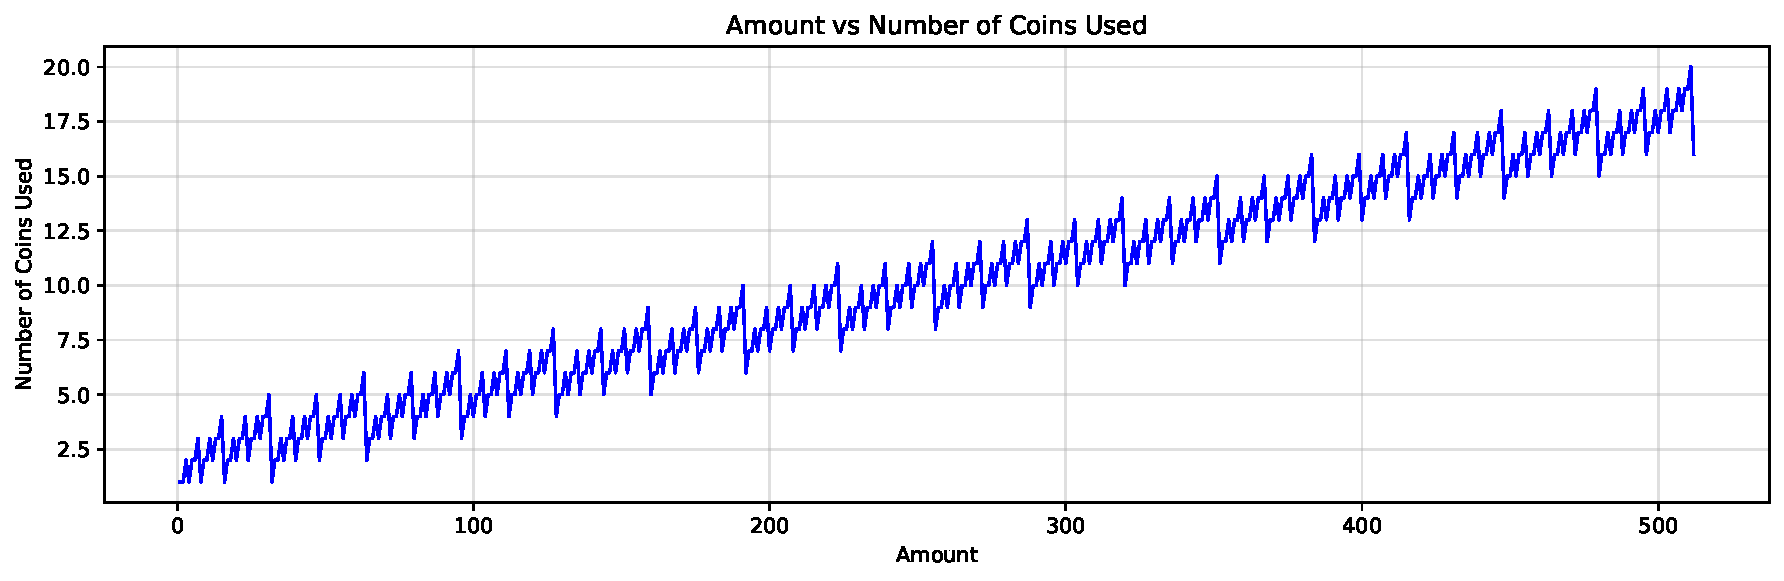
\includegraphics[width=\textwidth]{graphs/dp_coins_binary_plot.pdf}
  \caption{Number of coins used by the Dynamic Programming algorithm for the Binary coin system.}
  \label{fig:dp_coins_binary}
\end{figure}

\begin{figure}[H]
  \centering
  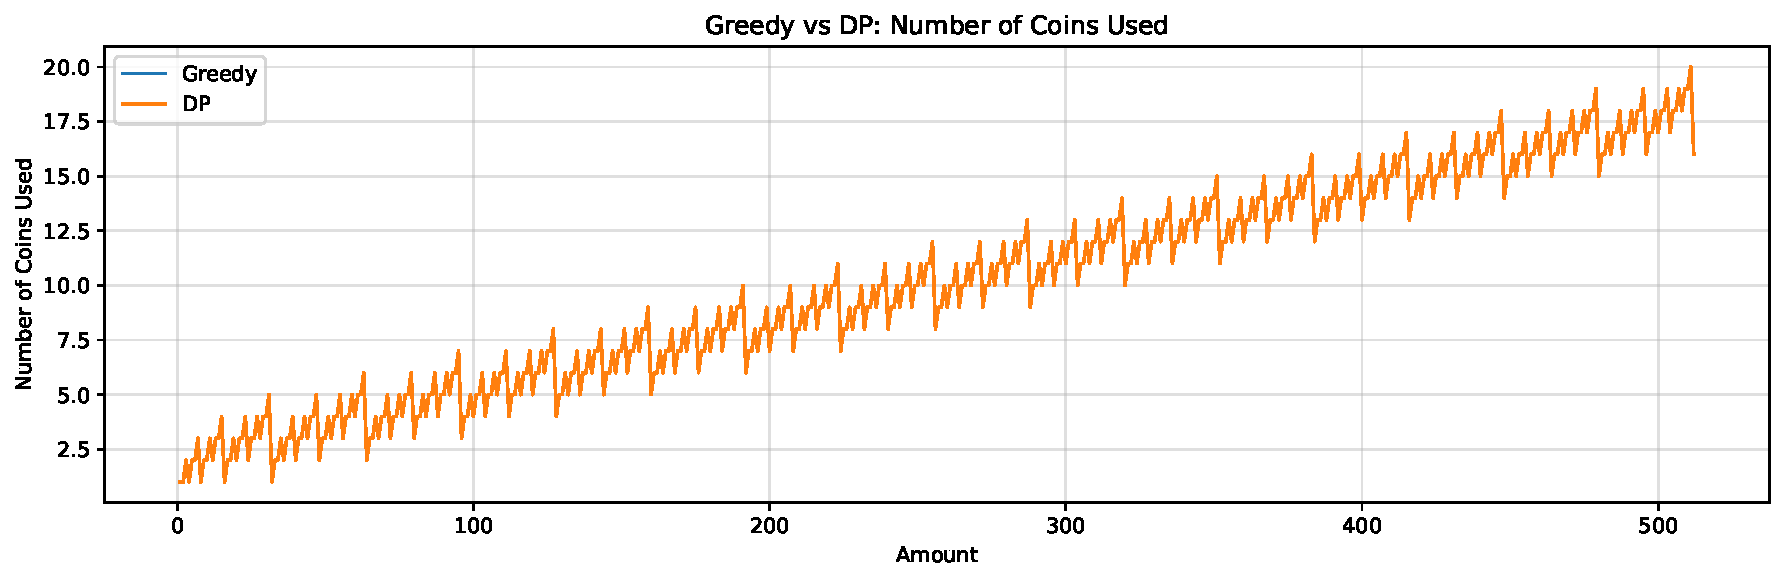
\includegraphics[width=\textwidth]{graphs/compare_coins_binary_plot.pdf}
  \caption{Comparison of minimum coins between Greedy and DP for the Binary coin system. Both algorithms produce identical results.}
  \label{fig:compare_coins_binary}
\end{figure}

\subsection{Decimal Coin System}
Denominations: [1, 10, 100], target range 1--1000. Greedy is optimal because each denomination is a multiple of smaller ones. Coin counts and execution time are consistent with theoretical predictions.

\begin{figure}[H]
  \centering
  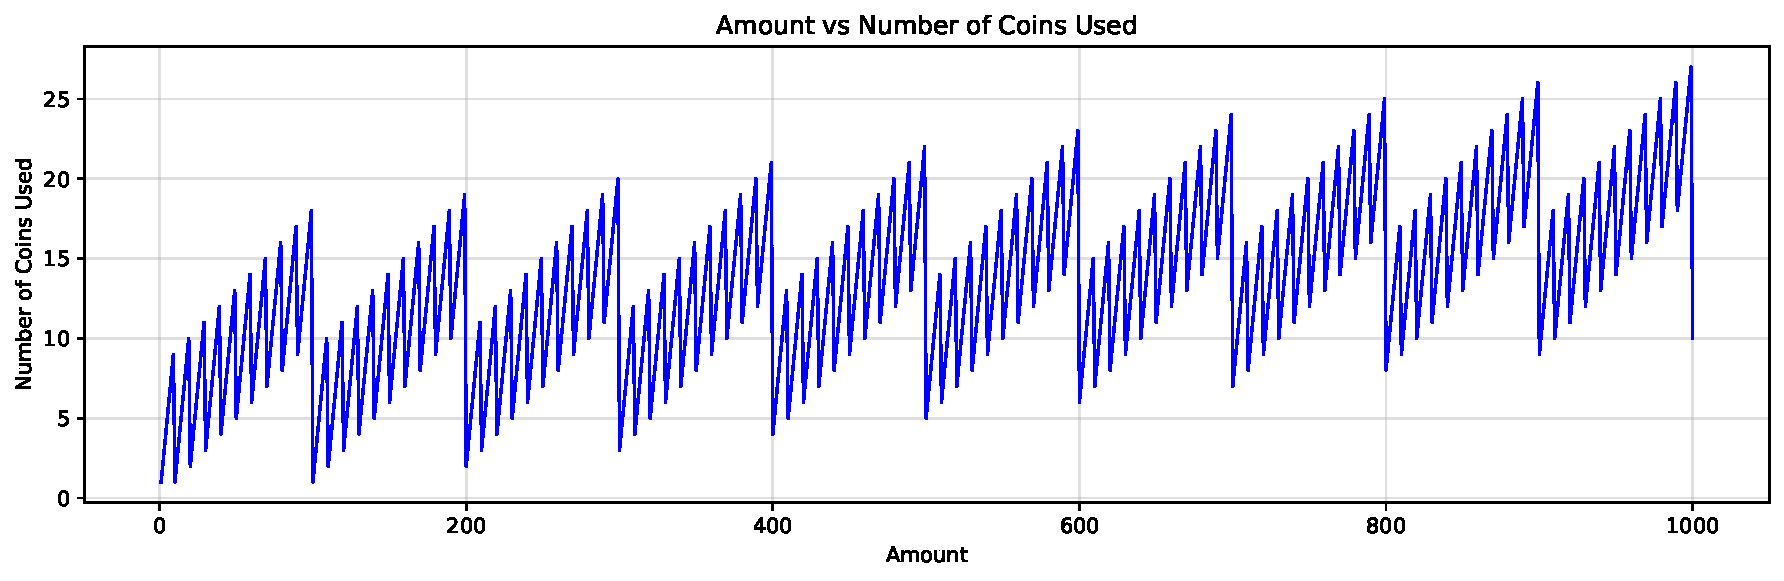
\includegraphics[width=\textwidth]{graphs/greedy_coins_decimal_plot.pdf}
  \caption{Number of coins used by the Greedy algorithm for the Decimal coin system.}
  \label{fig:greedy_coins_decimal}
\end{figure}

\begin{figure}[H]
  \centering
  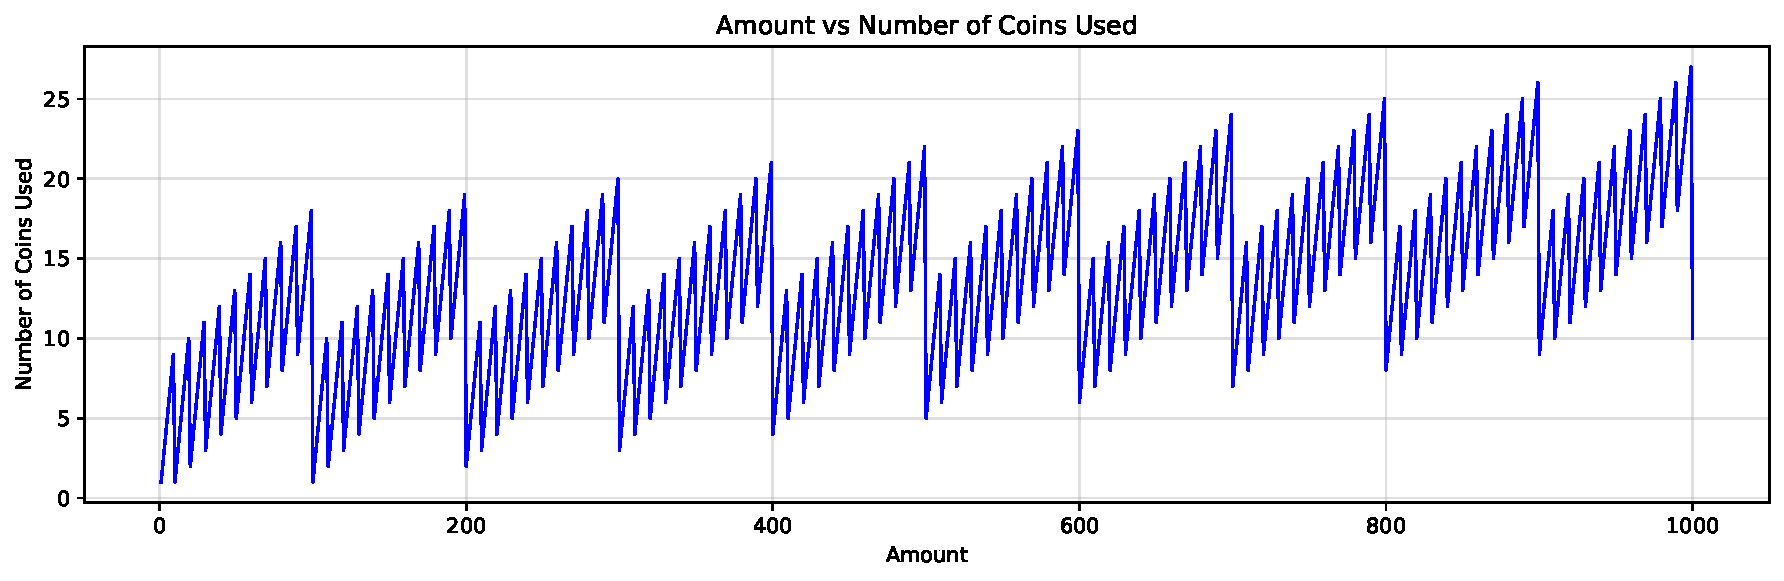
\includegraphics[width=\textwidth]{graphs/dp_coins_decimal_plot.pdf}
  \caption{Number of coins used by the Dynamic Programming algorithm for the Decimal coin system.}
  \label{fig:dp_coins_decimal}
\end{figure}

\begin{figure}[H]
  \centering
  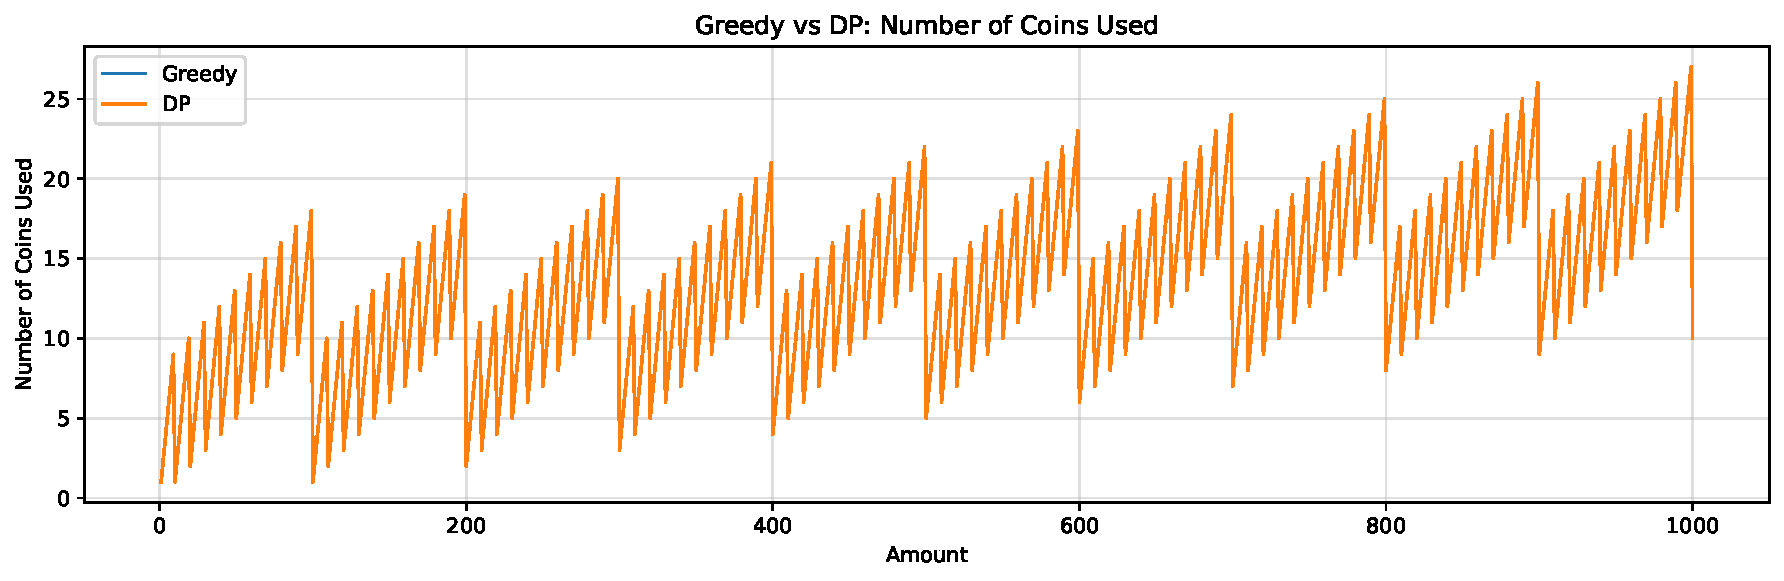
\includegraphics[width=\textwidth]{graphs/compare_coins_decimal_plot.pdf}
  \caption{Comparison of minimum coins between Greedy and DP for the Decimal coin system. Both algorithms produce identical results.}
  \label{fig:compare_coins_decimal}
\end{figure}

\subsection{Counting Coin System}
Denominations: [1, 2, 3, 4, 5, 6, 7], target range 1--100. Each denomination divides the next one, ensuring greedy optimality. Both algorithms match in coin counts.

\begin{figure}[H]
  \centering
  \includegraphics[width=\textwidth]{graphs/greedy_coins_counting_plot.pdf}
  \caption{Number of coins used by the Greedy algorithm for the Counting coin system.}
  \label{fig:greedy_coins_counting}
\end{figure}

\begin{figure}[H]
  \centering
  \includegraphics[width=\textwidth]{graphs/dp_coins_counting_plot.pdf}
  \caption{Number of coins used by the Dynamic Programming algorithm for the Counting coin system.}
  \label{fig:dp_coins_counting}
\end{figure}

\begin{figure}[H]
  \centering
  \includegraphics[width=\textwidth]{graphs/compare_coins_counting_plot.pdf}
  \caption{Comparison of minimum coins between Greedy and DP for the Counting coin system. Both algorithms produce identical results.}
  \label{fig:compare_coins_counting}
\end{figure}

\subsection{Observations}
\begin{itemize}
    \item For canonical systems, Greedy always produces the minimum number of coins, matching DP results.  
    \item Greedy is faster in execution time due to its iterative approach, while DP incurs overhead from table construction.  
    \item Graphs illustrate linear growth of coin count with target amount and predictable execution times.  
\end{itemize}

\section{Comparison on Non-Canonical Systems}
\label{sec:comparison_noncanonical}

This section compares Greedy and Dynamic Programming (DP) algorithms on non-canonical coin systems. Unlike canonical systems, Greedy may fail to produce the minimum number of coins, while DP always guarantees optimal results. We focus on three representative systems: Indian Coin System, Square Coin System, and Twin Prime Coin System. For each system, we highlight target amounts where Greedy fails and compare with DP.

\subsection{Old Indian Coin System}
Denominations: [1, 2, 5, 10, 20, 25, 50], target range 1--500. 

\begin{figure}[H]
  \centering
  \includegraphics[width=\textwidth]{graphs/greedy_coins_indiancoinsystum_plot.pdf}
  \caption{Number of coins used by the Greedy algorithm for the Indian Coin System. Certain targets are suboptimal.}
  \label{fig:greedy_coins_indiancoinsystem_plot}
\end{figure}

\begin{figure}[H]
  \centering
  \includegraphics[width=\textwidth]{graphs/dp_coins_indiancoinsystum_plot.pdf}
  \caption{Number of coins used by the DP algorithm for the Indian Coin System. DP always produces minimal coins.}
  \label{fig:dp_coins_indiancoinsystem_plot}
\end{figure}

\begin{figure}[H]
  \centering
  \includegraphics[width=\textwidth]{graphs/compare_coins_indiancoinsystum_plot.pdf}
  \caption{Comparison of Greedy vs DP for the Indian Coin System. Greedy fails on some targets, DP is always optimal.}
  \label{fig:compare_coins_indiancoinsystem_plot}
\end{figure}


\subsection{Square Coin System}
Denominations: [1, 4, 9, 16, 25, 36, 49], target range 1--441.

\begin{figure}[H]
  \centering
  \includegraphics[width=\textwidth]{graphs/greedy_coins_square_plot.pdf}
  \caption{Number of coins used by the Greedy algorithm for the Square coin system. Some targets are suboptimal.}
  \label{fig:greedy_coins_square_plot}
\end{figure}

\begin{figure}[H]
  \centering
  \includegraphics[width=\textwidth]{graphs/dp_coins_square_plot.pdf}
  \caption{Number of coins used by the DP algorithm for the Square coin system. DP always produces minimal coins.}
  \label{fig:dp_coins_square_plot}
\end{figure}

\begin{figure}[H]
  \centering
  \includegraphics[width=\textwidth]{graphs/compare_coins_square_plot.pdf}
  \caption{Comparison of Greedy vs DP for the Square coin system. DP always optimal; Greedy fails on certain targets.}
  \label{fig:compare_coins_square_plot}
\end{figure}


\subsection{Twin Prime Coin System}
Denominations: [1, 41, 43, 101, 103], target range 1--431.

\begin{figure}[H]
  \centering
  \includegraphics[width=\textwidth]{graphs/greedy_coins_twin_prime_plot.pdf}
  \caption{Number of coins used by the Greedy algorithm for the Twin Prime coin system. Some targets are suboptimal.}
  \label{fig:greedy_coins_twin_prime_plot}
\end{figure}

\begin{figure}[H]
  \centering
  \includegraphics[width=\textwidth]{graphs/dp_coins_twin_prime_plot.pdf}
  \caption{Number of coins used by the DP algorithm for the Twin Prime coin system. DP always produces minimal coins.}
  \label{fig:dp_coins_twin_prime_plot}
\end{figure}

\begin{figure}[H]
  \centering
  \includegraphics[width=\textwidth]{graphs/compare_coins_twin_prime_plot.pdf}
  \caption{Comparison of Greedy vs DP for the Twin Prime coin system. Greedy fails for some targets; DP always optimal.}
  \label{fig:compare_coins_twin_prime_plot}
\end{figure}

\subsection{Meme Coin System}
Denominations: [1, 6, 7, 69, 420], target range 1--666.

\begin{figure}[H]
  \centering
  \includegraphics[width=\textwidth]{graphs/greedy_coins_meme_plot.pdf}
  \caption{Number of coins used by the Greedy algorithm for the Meme coin system. Greedy fails for several targets due to non-canonical denominations.}
  \label{fig:greedy_coins_meme_plot}
\end{figure}

\begin{figure}[H]
  \centering
  \includegraphics[width=\textwidth]{graphs/dp_coins_meme_plot.pdf}
  \caption{Number of coins used by the DP algorithm for the Meme coin system. DP always yields the minimal number of coins.}
  \label{fig:dp_coins_meme_plot}
\end{figure}

\begin{figure}[H]
  \centering
  \includegraphics[width=\textwidth]{graphs/compare_coins_meme_plot.pdf}
  \caption{Comparison of Greedy vs DP for the Meme coin system. Greedy fails for targets such as 12, where it gives 6 coins instead of 2; DP remains optimal for all targets.}
  \label{fig:compare_coins_meme_plot}
\end{figure}

\subsection{Observations}
\begin{itemize}
    \item Greedy may fail to produce the minimum number of coins in non-canonical systems.  
    \item DP consistently produces the optimal number of coins for all targets.  
    \item Coin count comparison graphs clearly highlight targets where Greedy fails.  
    \item Execution time for Greedy remains slightly faster, but correctness cannot be assumed.
\end{itemize}

\section{Summary and Insights}
\label{sec:comparison_summary}

This chapter presented a detailed comparison between the Greedy and Dynamic Programming (DP) algorithms across both canonical and non-canonical coin systems.

\begin{itemize}
    \item \textbf{Canonical Systems:} In systems such as US Coin, Binary, Decimal, and Counting, Greedy produces the same minimal coin counts as DP. Execution time for Greedy is lower due to its simpler iterative method, making it efficient and correct for these systems.

    \item \textbf{Non-Canonical Systems:} Systems like the Old Indian Coin System, Square, Twin Prime and Meme show that Greedy may fail for certain targets. DP consistently yields the optimal number of coins, highlighting its necessity for correctness in non-canonical settings.

    \item \textbf{Trade-offs:} Greedy is faster and simpler but may not always minimize coins. DP guarantees minimal coins but has slightly higher computational and memory overhead.

    \item \textbf{Graphical Insights:} Coin count and execution time graphs illustrate where Greedy succeeds and fails. Linear trends appear in canonical systems, while deviations occur in non-canonical systems, reinforcing the theoretical analysis.
\end{itemize}

%~~~~~~~~~~~~~~~~~~~~~~~~~~~~~~~~~~~~~~~~~~~~~~~~~~~~~~~~~~~~~~~~~~~~~~~~~~~~~~~~~~~~~~~~~~~~~~~~~~~~~~~~~~~~~~~~~~~~~~~~~~~~~~~~~~~~~~~~~~~~~~~~~~~~~~~~~~~~~~~~~~~~~~~~~~~~~~~~~~~~~~~~~~~~~~~~~~~~~~~~~~~~~~~~~~~~~~~~~~~~~~~~~~~~~~~~~

\chapter{Real-World Application: Vending Machine Change Dispenser}
\section{Introduction}
Greedy algorithms are widely used in real-world applications where locally optimal choices lead to globally optimal solutions. One classic example is the \textit{coin change problem}, where the objective is to dispense a given amount using the minimal number of coins from available denominations.  

In this chapter, we demonstrate a practical implementation of the greedy algorithm through a \textbf{vending machine simulator}. The vending machine takes as input the amount of money paid and the cost of an item, and returns the remaining balance using the minimal number of coins.  

This example illustrates the efficiency and simplicity of the greedy approach in systems where the coin denominations allow an optimal solution through local decisions. It also provides a tangible link between the theoretical concepts discussed in previous chapters and a real-world scenario commonly encountered in daily life.

\section{Problem Description}
The goal of this section is to define the functionality of the vending machine and frame it as a coin change problem.  

\subsection{Task Definition}
The vending machine accepts payment for an item and returns the remaining balance using the fewest number of coins possible. 

\subsection{Simple Vending Machine}
For this example, we define a \textbf{Simple Vending Machine} as a machine that has an infinite supply of coins for each denomination.  

Because of this assumption, the greedy algorithm is sufficient to compute the minimal set of coins for any remaining balance. There is no need for additional calculations, backtracking, or dynamic programming, as the availability of unlimited coins guarantees that the largest possible denominations can always be used first.  

This simplifies the real-world implementation and ensures that the algorithm always produces an optimal solution for standard coin systems, such as the Indian denominations of  Rs.~100, Rs.~5,	 Rs.~2, and Rs.~1.

\subsection{Inputs and Outputs}
\begin{itemize}
    \item \textbf{Input:} 
    \begin{itemize}
        \item \textit{Amount Paid} (\texttt{amount\_paid}): total money given by the user.
        \item \textit{Cost of Item} (\texttt{cost}): price of the selected item.
    \end{itemize}
    \item \textbf{Output:} 
    \begin{itemize}
        \item A list of coins representing the remaining balance, using the minimal number of coins.
    \end{itemize}
\end{itemize}

\subsection{Assumptions}
\begin{itemize}
    \item Available coin denominations are fixed and known, for example: Rs.~10, Rs.~5, Rs.~2, and Rs.~1.
    \item The amount paid is always greater than or equal to the cost of the item.
    \item The machine has an unlimited supply of each denomination.
\end{itemize}

\subsection{Example Scenario}
If a user pays Rs.~150 for an item costing Rs.~104, the remaining balance is Rs.~46. The vending machine should dispense this amount using the fewest coins possible, which can be represented as: \{Rs.~20 × Rs.~2, Rs.~5 × 1, Rs.~1 × 1\}.
\section{Greedy Algorithm Logic}
The greedy algorithm solves the coin change problem by always selecting the largest coin denomination that does not exceed the remaining amount. This local choice is repeated until the balance becomes zero.

\subsection{Algorithm Steps}
\begin{enumerate}
    \item Compute the remaining balance:
    \[
        \text{balance} = \text{amount\_paid} - \text{cost}
    \]
    \item Initialize an empty list to store the coins to be dispensed.
    \item While the balance is greater than zero:
    \begin{enumerate}
        \item Pick the largest coin denomination less than or equal to the balance.
        \item Subtract its value from the balance.
        \item Add the coin to the dispensed coins list.
    \end{enumerate}
    \item Return the list of coins.
\end{enumerate}


\subsection{Pseudocode}
\begin{algorithm}
\caption{Greedy Algorithm for Vending Machine Coin Change}
\begin{algorithmic}[1]
\Procedure{DispenseChange}{$coins, amount\_paid, cost$}
    \State \Comment{$coins$ is sorted in descending order}
    \State $balance \gets amount\_paid - cost$
    \State $dispensed \gets [\ ]$ \Comment{List to store coins}
    
    \For{$coin \in coins$}
        \While{$balance \ge coin$}
            \State $balance \gets balance - coin$ \Comment{Reduce remaining balance}
            \State append $coin$ to $dispensed$
        \EndWhile
    \EndFor
    
    \If{$balance = 0$}
        \State \Return $dispensed$ \Comment{Return list of coins}
    \Else
        \State \Return \texttt{error} \Comment{Target cannot be formed with given coins}
    \EndIf
\EndProcedure
\end{algorithmic}
\end{algorithm}

\section{Implementation}
This section provides a Python implementation of the greedy coin change algorithm for the vending machine scenario. The function \texttt{dispense\_change} takes the amount paid, the cost of the item, and a list of available coin denominations, and returns the minimal set of coins for the remaining balance.

\subsection{Python Implementation}

\lstinputlisting[caption={Python implementation of Simple Vending machine},label={lst:vendingMachine}]{code/vendingMachine.py}

\subsection{Example Usage}
\begin{verbatim}
# Example: User pays 150 for an item worth 104
change = dispense_change(150, 104)
print(change)  # Output: [20, 20, 5, 1]
\end{verbatim}
The algorithm correctly returns the minimal number of coins for the balance, demonstrating the efficiency of the greedy approach in a real-world scenario.

\section{Example Execution}
This section demonstrates the greedy coin change algorithm in action for the Simple Vending Machine.  

\subsection{Scenario}
A user purchases an item costing Rs.~104 and pays Rs.~150. The vending machine must return Rs.~46 using the minimal number of coins.  

\subsection{Greedy Coin Selection}
\begin{itemize}
    \item Available denominations: Rs.~10, Rs.~5, Rs.~2, Rs.~1
    \item Remaining balance: Rs.~46
\end{itemize}

The algorithm selects coins in descending order:

\begin{center}
\begin{tabular}{c c c}
\hline
Coin & Quantity & Remaining Balance \\
\hline
Rs.~20 & 2 & 46 - 40 = 6 \\
Rs.~5 & 1 & 6 - 5 = 1 \\
Rs.~1 & 1 & 1 - 1 = 0 \\
\hline
\end{tabular}
\end{center}

\subsection{Result}
The machine dispenses the coins: \{Rs.~20 × 2, Rs.~5 × 1, Rs.~1 × 1\}.  

\section{Conclusion}
In this chapter, we demonstrated a real-world application of the greedy algorithm through a Simple Vending Machine that returns change using minimal coins.  

Key takeaways:
\begin{itemize}
    \item The greedy algorithm efficiently computes the minimal set of coins when the machine has an infinite supply of standard denominations.
    \item For canonical coin systems, such as Indian coins (Rs.~10, Rs.~5, Rs.~2, Rs.~1), greedy guarantees an optimal solution.
    \item The example highlights the practicality of greedy algorithms in embedded systems like vending machines, ATMs, and kiosks, where simplicity and speed are essential.
    \item Limitations arise only when coin systems are non-canonical or supply is restricted, which would require more advanced algorithms.
\end{itemize}

This implementation bridges the gap between theoretical concepts of the coin change problem and real-world scenarios, illustrating how algorithmic design principles are applied in everyday technology.

%++++++++++++++++++++++++++++++++++++++++++++++++++++++++++++++++++++++++++++++++++++++++++++++++++++++++++++++++++++++++++++++++++++++++++++++++++++++++++++++++++++++++++++++++++++++++++++++++++++++++++++++++++++++++++++++++++++++++

\chapter{The Greedy Way to Handle Vault Hunter Coins}
\section{Introduction}

In the \textit{Vault Hunter} mod of \textit{Minecraft}, players earn an in-game physical currency which consists of four denominations: bronze, silver, gold, and platinum coins. Efficient management of this currency is crucial due to the limited inventory space and frequent transactions with game vendors or other players. 

The in-game currency system is hierarchical, with each higher denomination representing a multiple of the lower denomination:
\begin{itemize}
    \item 1 silver coin = 9 bronze coins,
    \item 1 gold coin = 9 silver coins = 81 bronze coins,
    \item 1 platinum coin = 9 gold coins = 729 bronze coins.
\end{itemize}

During transactions, players must provide an exact amount of currency, and the system returns the balance in appropriate coins. Carrying too many low-value coins can clutter the inventory and slow down gameplay, while carrying high-value coins efficiently reduces the total number of coins. 

This chapter explores the application of the \textbf{greedy coin change algorithm} to determine the optimal combination of platinum, gold, silver, and bronze coins to give as change. The greedy approach ensures that the number of coins carried is minimized, which is particularly well-suited to the Vault Hunter currency system due to its canonical nature, where each denomination is a multiple of the previous one. Through this practical example, we demonstrate how algorithmic strategies can enhance both game efficiency and player experience.

\section{Problem Statement}

In the \textit{Vault Hunter} mod of \textit{Minecraft}, players handle four denominations of currency: bronze, silver, gold, and platinum coins. Each transaction requires giving or receiving a specific amount of currency, and the game system automatically provides the balance in the available denominations.  

The problem can be formally stated as follows:

\begin{quote}
\textbf{Given:} An amount of currency expressed in bronze coins (or any combination of platinum, gold, silver, and bronze), and the conversion rates:
\begin{itemize}
    \item 1 silver = 9 bronze
    \item 1 gold = 9 silver = 81 bronze
    \item 1 platinum = 9 gold = 729 bronze
\end{itemize}

\textbf{Objective:} Determine the minimum number of coins (platinum, gold, silver, bronze) required to represent the amount accurately, so that:
\begin{itemize}
    \item The total value of coins equals the target amount.
    \item Inventory space is minimized by reducing the total number of coins carried.
    \item The combination is suitable for quick and efficient transactions.
\end{itemize}
\end{quote}

\noindent In other words, for any given transaction amount, we need to calculate how many platinum, gold, silver, and bronze coins should be given or returned so that the player carries the fewest possible coins while maintaining exact value.  

This problem is a natural application of the \textbf{coin change problem}, where we aim to find the optimal coin combination. Due to the canonical nature of the Vault Hunter currency system, where each higher denomination is a multiple of the lower, the greedy algorithm is guaranteed to produce an optimal solution.

\section{Greedy Algorithm Overview}

The \textit{greedy algorithm} is a natural strategy for solving the coin change problem in the Vault Hunter currency system. The key idea of the greedy approach is simple: at each step, choose the largest coin denomination that does not exceed the remaining amount. This process is repeated until the entire amount is represented.  

\subsection{Why Greedy Works Here}

The greedy algorithm guarantees an optimal solution in this case because the Vault Hunter currency is \textbf{canonical}: each higher denomination is an exact multiple of the lower denomination:
\[
1 \text{ platinum} = 9 \text{ gold} = 81 \text{ silver} = 729 \text{ bronze}.
\]
This property ensures that using the largest possible coin at each step minimizes the total number of coins, making the greedy choice optimal.

\subsection{Algorithm Steps}

For a given amount of currency (in bronze coins), the greedy algorithm proceeds as follows:

\begin{enumerate}
    \item Start with the highest denomination, platinum.
    \item Determine how many platinum coins fit into the amount:
    \[
    \text{num\_platinum} = \left\lfloor \frac{\text{amount}}{729} \right\rfloor
    \]
    and subtract their value from the total amount.
    \item Repeat the same process for gold (81 bronze), silver (9 bronze), and finally bronze (1 bronze).
    \item The remaining amount after distributing all higher denominations will automatically be represented by bronze coins.
\end{enumerate}

\subsection{Pseudocode}
\begin{algorithm}
\caption{Greedy Algorithm for Vault Hunter Coin Change}
\begin{algorithmic}[1]
\Procedure{DispenseChange}{$coins, amount\_paid, cost$}
    \State \Comment{$coins$ is sorted in descending order: platinum, gold, silver, bronze}
    \State $balance \gets amount\_paid - cost$
    \State $dispensed \gets [\ ]$ \Comment{List to store coins to give as change}
    
    \For{$coin \in coins$}
        \While{$balance \ge coin$}
            \State $balance \gets balance - coin$ \Comment{Reduce remaining balance}
            \State append $coin$ to $dispensed$ \Comment{Give one coin of this denomination}
        \EndWhile
    \EndFor
    
    \If{$balance = 0$}
        \State \Return $dispensed$ \Comment{Return exact change in minimum coins}
    \Else
        \State \Return \texttt{error} \Comment{Cannot form target amount with available coins}
    \EndIf
\EndProcedure
\end{algorithmic}
\end{algorithm}

\noindent This algorithm efficiently computes the minimum number of coins for any given amount and ensures that the player carries the fewest coins possible during in-game transactions.

\section{Real-World Analogy in Vault Hunter}

In \textit{Vault Hunter}, players frequently earn and spend in-game currency while exploring dungeons, trading with NPCs, or completing quests. Efficient coin management is essential because players have limited inventory space, and carrying too many low-value coins (bronze or silver) can clutter their inventory and slow down gameplay.  

The greedy coin change algorithm provides a practical solution for these transactions by minimizing the number of coins a player must carry. Each transaction can be thought of as a real-world scenario:

\subsection{Scenario Example}

Suppose a player receives a total of 3452 bronze coins from various quests. To carry these coins efficiently, the player wants to convert them into higher denominations wherever possible:

\begin{itemize}
    \item \textbf{Platinum coins:} $\lfloor 3452 / 729 \rfloor = 4$ (remaining: $3452 - 4 \times 729 = 676$)  
    \item \textbf{Gold coins:} $\lfloor 676 / 81 \rfloor = 8$ (remaining: $676 - 8 \times 81 = 28$)  
    \item \textbf{Silver coins:} $\lfloor 28 / 9 \rfloor = 3$ (remaining: $28 - 3 \times 9 = 1$)  
    \item \textbf{Bronze coins:} $1$  
\end{itemize}

\noindent The resulting distribution is:
\[
4 \text{ platinum}, \quad 8 \text{ gold}, \quad 3 \text{ silver}, \quad 1 \text{ bronze.}
\]

This combination minimizes the total number of coins (16 coins in total) and ensures that the player can carry all currency efficiently during further transactions.

\subsection{Inventory Table Representation}

To visualize how the coins are stored in the inventory, the following table can be used:

\begin{center}
\begin{tabular}{|c|c|c|}
\hline
\textbf{Coin Type} & \textbf{Value (in bronze)} & \textbf{Quantity} \\
\hline
Platinum & 729 & 4 \\
Gold & 81 & 8 \\
Silver & 9 & 3 \\
Bronze & 1 & 1 \\
\hline
\end{tabular}
\end{center}

\noindent By following this greedy approach for all transactions, players can quickly calculate the change to give or receive, minimize coin clutter, and make trading with NPCs or other players faster and more efficient.

\subsection{Gameplay Benefits}

\begin{itemize}
    \item \textbf{Minimal inventory usage:} Carrying fewer coins leaves space for other valuable items like weapons, potions, or loot.  
    \item \textbf{Faster transactions:} Giving or receiving the exact change in higher denominations reduces time spent counting coins.  
    \item \textbf{Optimal currency management:} Ensures that players always have the correct balance for future trades without unnecessary low-value coins.  
\end{itemize}

This real-world analogy demonstrates how the greedy coin change algorithm is not only a theoretical problem but also a practical tool for improving gameplay efficiency in Vault Hunter.

\section{Implementation}

The greedy coin change algorithm can be implemented practically in Python to handle Vault Hunter transactions efficiently. In this implementation, both the amount paid and the cost of an item can be expressed using any combination of coins: platinum, gold, silver, and bronze. The algorithm then computes the optimal change in the fewest number of coins.

\subsection{Python Implementation}

The Python script \texttt{vaultHunter.py} contains the function \texttt{compute\_vault\_coin}, which calculates the number of coins to return as change. The function accepts two dictionaries: \texttt{amount\_paid} and \texttt{cost}, each specifying the number of coins of each type. The function returns a dictionary representing the change to give in platinum, gold, silver, and bronze coins.

\lstinputlisting[caption={Python implementation of Vault Hunter Coin Change},label={lst:vaultHunter}]{code/vaultHunter.py}

\subsection{Documentation of the Script}

\begin{itemize}
    \item \textbf{Function:} \texttt{compute\_vault\_coin(amount\_paid, cost)}
    \begin{itemize}
        \item \textbf{amount\_paid:} Dictionary specifying coins paid, e.g.,
        \texttt{\{'platinum': 2, 'gold': 0, 'silver': 3, 'bronze': 5\}}
        \item \textbf{cost:} Dictionary specifying the cost in the same format
        \item \textbf{Returns:} Dictionary with keys \texttt{'platinum', 'gold', 'silver', 'bronze'} showing the number of coins to return, or \texttt{'error'} if total payment is insufficient
    \end{itemize}
    \item \textbf{Algorithm:}
    \begin{enumerate}
        \item Convert both \texttt{amount\_paid} and \texttt{cost} into total bronze units using the coin conversion rates:
         \[
        1 \text{ platinum} = 729 \text{ bronze}, \quad
        1 \text{ gold} = 81 \text{ bronze},
        \]
        \[
        1 \text{ silver} = 9 \text{ bronze}, \quad
        1 \text{ bronze} = 1 \text{ bronze}
        \]
        \item Compute the balance: \texttt{balance = total\_paid - total\_cost}.
        \item If the balance is negative, return \texttt{'error'}.
        \item Use the greedy algorithm to determine the number of coins of each denomination to return as change, starting from the largest (platinum) to the smallest (bronze).
    \end{enumerate}
    \item \textbf{Example:}  
    Suppose a player pays:
    \[
    \texttt{amount\_paid = \{'platinum': 5, 'gold': 0, 'silver': 2, 'bronze': 0\}}
    \]  
    for an item costing:
    \[
    \texttt{cost = \{'platinum': 1, 'gold': 3, 'silver': 2, 'bronze': 5\}}
    \]  
    The function computes the change as:
    \[
    \texttt{\{'platinum': 3, 'gold': 5, 'silver': 8, 'bronze': 4\}}
    \]  
    which is the minimum number of coins required.
\end{itemize}

This implementation allows players to manage Vault Hunter currency efficiently, handling transactions of any denomination and ensuring minimal inventory usage while providing exact change.

\section{Analysis}

The greedy coin change algorithm for Vault Hunter transactions is both efficient and optimal due to the canonical nature of the in-game currency system. This section analyzes its correctness, time complexity, and practical implications.

\subsection{Correctness}

The algorithm is guaranteed to produce an optimal solution (i.e., the minimum number of coins) because the Vault Hunter coin denominations satisfy the canonical property:
\[
1 \text{ silver} = 9 \text{ bronze}, \quad
1 \text{ gold} = 9 \text{ silver} = 81 \text{ bronze}, \quad
1 \text{ platinum} = 9 \text{ gold} = 729 \text{ bronze}.
\]

\noindent In such a system, at each step, selecting the largest coin denomination that does not exceed the remaining balance ensures that no smaller combination of coins can use fewer total coins. This is the fundamental principle behind the greedy approach.

\subsection{Time Complexity}

Let $n$ be the number of coin denominations. In Vault Hunter, $n = 4$ (platinum, gold, silver, bronze). The algorithm iterates over each denomination exactly once, performing a constant-time operation (\texttt{divmod}) for each:

\[
\text{Time complexity: } O(n)
\]

Since $n$ is constant, the algorithm runs in \textbf{constant time} in practice, making it highly efficient for real-time gameplay transactions.

\subsection{Space Complexity}

The algorithm maintains a small dictionary to store the number of coins for each denomination:

\[
\text{Space complexity: } O(n)
\]

Again, since $n$ is fixed at 4, the space usage is minimal and suitable for in-game computation.

\subsection{Practical Implications for Vault Hunter}

\begin{itemize}
    \item \textbf{Minimal inventory usage:} Players carry fewer coins, freeing up space for other valuable items.
    \item \textbf{Fast transactions:} Both giving and receiving change can be computed instantly.
    \item \textbf{Exact change guaranteed:} The greedy algorithm ensures that any amount can be correctly represented in coins.
    \item \textbf{Scalability:} Even if future mods introduce more denominations following canonical multiples, the algorithm adapts easily.
\end{itemize}

\subsection{Limitations}

The greedy approach relies on the canonical property. If the game introduces non-canonical coins (e.g., a 10-bronze coin), the algorithm may no longer guarantee the minimum number of coins, and a dynamic programming approach would be necessary.

\noindent In the current Vault Hunter currency system, however, the greedy algorithm is both optimal and extremely practical.

\section{Conclusion}

In this chapter, we explored the practical application of the greedy coin change algorithm within the \textit{Vault Hunter} mod of \textit{Minecraft}. The in-game currency system—comprising bronze, silver, gold, and platinum coins—follows a canonical structure, where each higher denomination is a multiple of the lower. This property allows the greedy algorithm to compute the minimum number of coins needed for any transaction efficiently and accurately.

We demonstrated how both the amount paid and the cost of an item can be specified in any combination of coins, and the algorithm returns the optimal distribution of change. The implementation ensures minimal inventory usage, fast transactions, and exact change for the player, thereby enhancing gameplay experience.

Key takeaways include:

\begin{itemize}
    \item The greedy algorithm guarantees an optimal solution for canonical coin systems.  
    \item Time complexity is $O(n)$ and space complexity is $O(n)$, with $n$ being the number of coin denominations.  
    \item The approach is practical for real-time in-game transactions and scales well if additional denominations are added, provided they maintain the canonical property.  
    \item Limitations exist when non-canonical denominations are introduced, where a dynamic programming solution may be required.  
\end{itemize}

Overall, the greedy coin change algorithm provides a simple yet powerful strategy for effective currency management in Vault Hunter, combining algorithmic efficiency with tangible in-game benefits. This real-world example illustrates how classical algorithms can enhance gameplay mechanics and user experience in video games.


\begin{thebibliography}{99}

\bibitem{cai2008}
Xuan Cai.  
\textit{Canonical Coin Systems for Change-Making Problems.} arXiv preprint arXiv:0809.0400, 2008.  
\url{https://arxiv.org/pdf/0809.0400}

\bibitem{cormen}
Cormen, T. H., Leiserson, C. E., Rivest, R. L., and Stein, C.  
\textit{Introduction to Algorithms}, 3rd Edition.  
MIT Press, 2009.

\bibitem{gfg}
GeeksforGeeks.  
\textit{Understanding the Coin Change Problem with Dynamic Programming.}  
\url{https://www.geeksforgeeks.org/dsa/understanding-the-coin-change-problem-with-dynamic-programming}  
Accessed Oct 19, 2025.

\bibitem{takeuforward}
Take U Forward.  
\textit{Minimum Coins | Greedy Algorithms.} YouTube, Feb 4, 2021.  
\url{https://www.youtube.com/watch?v=mVg9CfJvayM&t}

\end{thebibliography}


\end{document}
